\documentclass[11pt,letterpaper,openany]{book}
\usepackage[T1]{fontenc}
\usepackage[sc]{mathpazo}
\usepackage[scaled=0.92]{helvet}
\linespread{1.06}
\usepackage[margin=0.9in,top=0.85in,bottom=0.9in,headheight=14pt]{geometry}
\usepackage{amsmath,amssymb,mathtools,bm}
\usepackage{graphicx,xcolor,tabularx,booktabs,array,multicol,enumitem,longtable}
\usepackage[most]{tcolorbox}
\usepackage{titlesec,fancyhdr}
\usepackage{siunitx}
\usepackage[hidelinks,pdftitle={LiDAR from the Ground Up},pdfauthor={D.S. Banks, PSM}]{hyperref}
\graphicspath{{figs/}}
\setlist{itemsep=1pt,topsep=3pt}
\setlength{\parskip}{4pt}\setlength{\parindent}{0pt}

\definecolor{navy}{HTML}{1F3B73}\definecolor{teal}{HTML}{138D75}\definecolor{orange}{HTML}{E67E22}
\definecolor{red}{HTML}{C0392B}\definecolor{purple}{HTML}{7D3C98}\definecolor{gold}{HTML}{B7950B}
\definecolor{kid}{HTML}{1E8449}\definecolor{grayx}{HTML}{5D6D7E}

% headings
\titleformat{\chapter}[display]{\sffamily\bfseries\color{navy}}{\large MODULE \thechapter}{4pt}{\Huge}[\vspace{2pt}{\color{orange}\titlerule[2pt]}]
\titlespacing*{\chapter}{0pt}{-10pt}{14pt}
\titleformat{\section}{\sffamily\Large\bfseries\color{navy}}{\thesection}{0.6em}{}
\titleformat{\subsection}{\sffamily\large\bfseries\color{teal}}{\thesubsection}{0.6em}{}
\titlespacing*{\section}{0pt}{10pt}{4pt}\titlespacing*{\subsection}{0pt}{8pt}{3pt}

\pagestyle{fancy}\fancyhf{}
\fancyhead[L]{\sffamily\small\color{grayx}LiDAR from the Ground Up}
\fancyhead[R]{\sffamily\small\color{grayx}\leftmark}
\fancyfoot[C]{\sffamily\small\thepage}
\renewcommand{\headrulewidth}{0.4pt}
\renewcommand{\chaptermark}[1]{\markboth{Module \thechapter: #1}{}}
\fancypagestyle{plain}{\fancyhf{}\fancyfoot[C]{\sffamily\small\thepage}\renewcommand{\headrulewidth}{0pt}}

% boxes
\tcbset{base/.style={enhanced,breakable,boxrule=0.8pt,arc=3pt,left=7pt,right=7pt,top=5pt,bottom=5pt,fonttitle=\sffamily\bfseries,before skip=8pt,after skip=8pt}}
\newtcolorbox{kid}[1][]{base,colback=kid!6,colframe=kid,title={\textsf{SIMPLE APPROACH}},#1}
\newtcolorbox{eng}[1][]{base,colback=navy!4,colframe=navy,title={\textsf{ENGINEER'S VIEW}},#1}
\newtcolorbox{worked}[1]{base,colback=orange!5,colframe=orange,title={WORKED EXAMPLE --- #1}}
\newtcolorbox{tryit}[1][]{base,colback=purple!5,colframe=purple,title={TRY IT YOURSELF},after upper={\par\smallskip{\color{purple}\rule{\linewidth}{0.4pt}}\par\textsf{\small\color{purple}\textbf{Answers:} worked solutions are in Appendix A, ``Answers to Try It Yourself,'' starting on page \pageref{app:answers}.}},#1}
\newtcolorbox{improve}[1][]{base,colback=red!4,colframe=red!80!black,title={IMPROVED FROM THE SOURCE MATERIAL},#1}
\newtcolorbox{tip}[1][]{base,colback=teal!6,colframe=teal,title={SURVEYOR'S FIELD TIP},#1}
\newtcolorbox{keyeq}[1]{base,unbreakable,colback=white,colframe=navy,boxrule=1.4pt,title={KEY EQUATION --- #1},coltitle=white,colbacktitle=navy}
\newtcolorbox{seminar}[1][]{base,colback=gold!8,colframe=gold!80!black,boxrule=1.4pt,title={FOR SURVEY SEMINAR PARTICIPANTS},#1}
\newtcolorbox{warning}[1][]{base,colback=red!6,colframe=red!75!black,boxrule=1.4pt,title={WARNING},#1}
\newtcolorbox{bigidea}{base,colback=gold!10,colframe=gold,title={BIG IDEA}}

\newcommand{\step}[1]{\par\smallskip\textsf{\textbf{\color{orange!80!black}#1}}\par}
\newcommand{\result}[1]{\par\smallskip\colorbox{orange!20}{\parbox{\dimexpr\linewidth-2\fboxsep}{\textbf{Result:} #1}}\par}
\newenvironment{symbols}{\par\smallskip\textsf{\small\textbf{What every symbol means}}\par\small\renewcommand{\arraystretch}{1.15}\tabularx{\linewidth}{>{\centering\arraybackslash}p{1.6cm}X>{\raggedright\arraybackslash}p{2.4cm}}\toprule\textbf{Symbol}&\textbf{Meaning}&\textbf{Units}\\\midrule}{\bottomrule\endtabularx\par}
\newcommand{\fig}[3][0.9]{\begin{figure}[htbp]\centering\includegraphics[width=#1\linewidth]{#2}\caption{#3}\end{figure}}
\usepackage{caption}\captionsetup{font={small,sf},labelfont={bf,color=navy}}
\newcommand{\vect}[1]{\mathbf{#1}}
\newcommand{\sources}[1]{\begin{tcolorbox}[base,colback=gray!4,colframe=grayx,title={SOURCES FOR THIS MODULE}]\footnotesize #1\end{tcolorbox}}

\raggedbottom
\renewcommand{\topfraction}{0.85}\renewcommand{\textfraction}{0.1}\renewcommand{\floatpagefraction}{0.75}
\begin{document}
\frontmatter
\begin{titlepage}
\begin{tikzpicture}[remember picture,overlay]
\fill[fill={rgb,255:red,26;green,50;blue,99}] (current page.south west) rectangle (current page.north east);
\node[anchor=center] at ([yshift=-0.9in]current page.center) {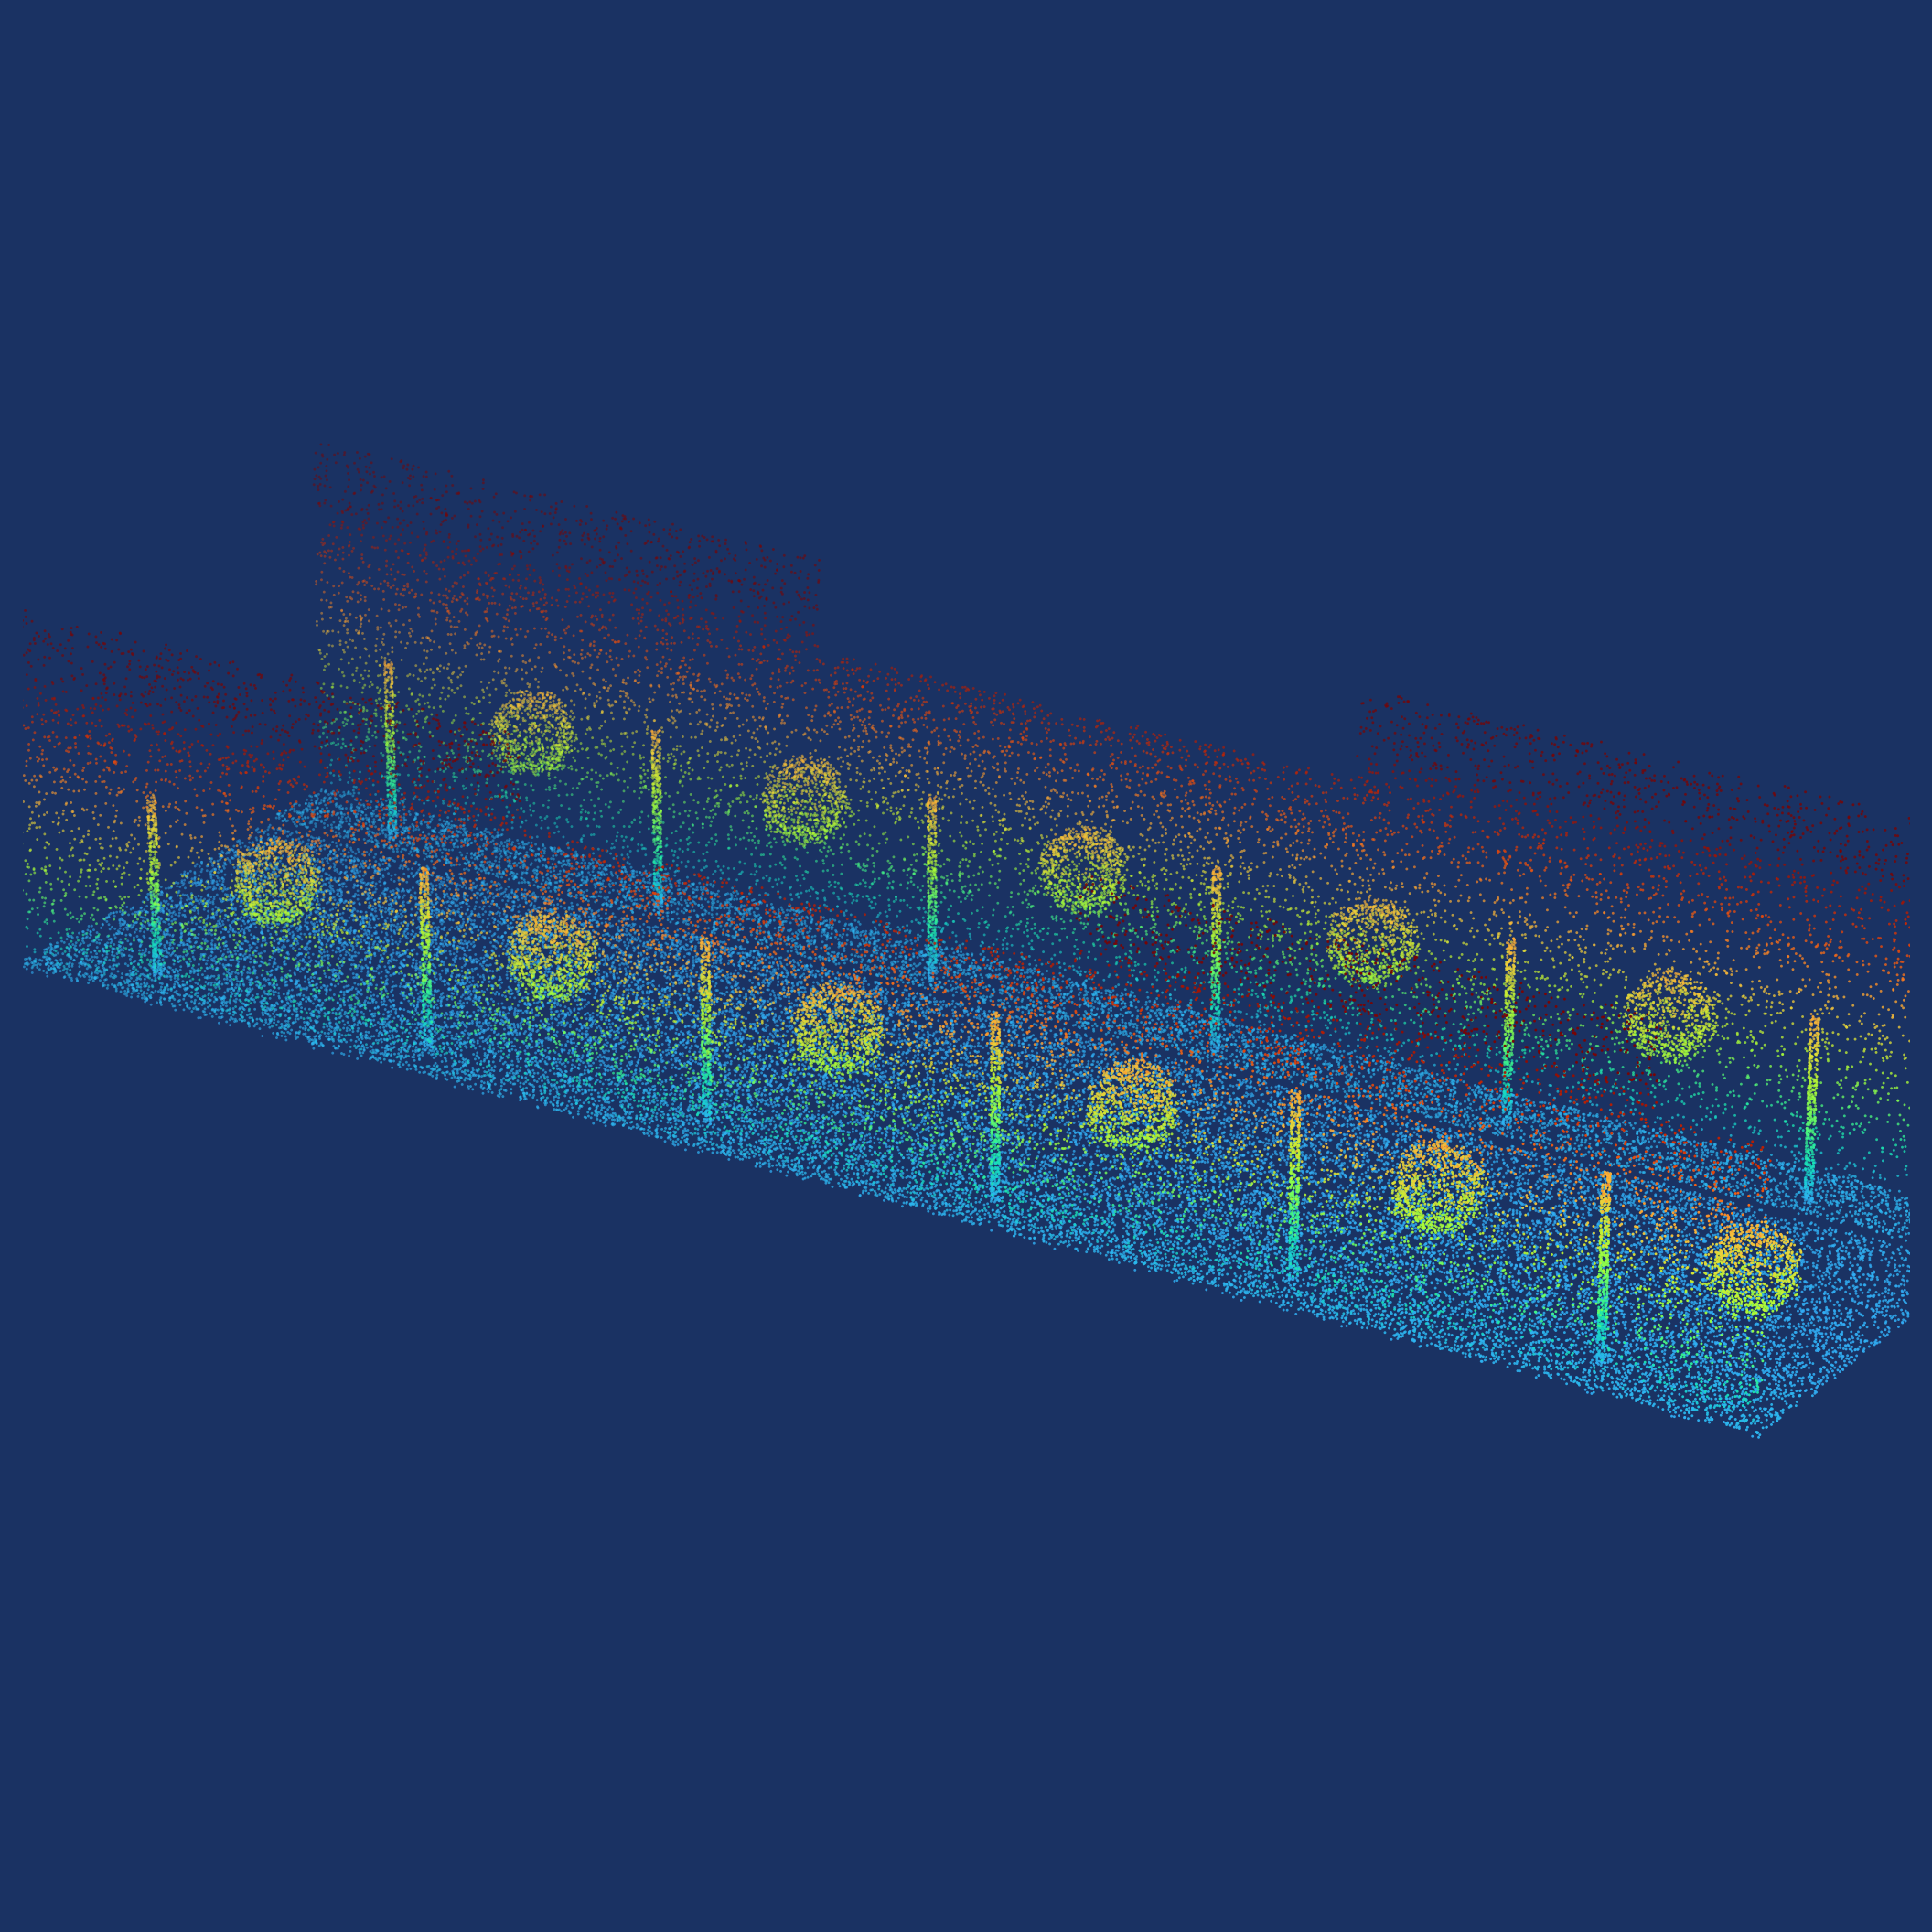
\includegraphics[width=\paperwidth]{cover}};
\fill[orange] ([yshift=-3.05in]current page.north west) rectangle ([yshift=-3.12in]current page.north east);
\node[anchor=north west,text width=7in,align=left] at ([xshift=0.75in,yshift=-0.8in]current page.north west)
 {\color{white}\sffamily\bfseries\fontsize{40}{46}\selectfont\spaceskip=0.28em LiDAR from the Ground Up};
\node[anchor=north west,text width=7in,align=left] at ([xshift=0.75in,yshift=-1.65in]current page.north west)
 {\color{orange!60}\sffamily\Large Mobile Laser Scanning, IMUs, SLAM and Survey-Grade Deliverables};
\node[anchor=north west,text width=7in,align=left] at ([xshift=0.75in,yshift=-2.05in]current page.north west)
 {\color{white}\sffamily\bfseries\LARGE D.S. Banks, PSM};
\node[anchor=north west,text width=7in,align=left] at ([xshift=0.75in,yshift=-2.55in]current page.north west)
 {\color{white!85}\sffamily\large A two-track course: a simple approach anyone can follow,\\ and a rigorous engineering treatment --- on every topic.};
\node[anchor=south west,text width=7in,align=left] at ([xshift=0.75in,yshift=0.8in]current page.south west)
 {\color{white}\sffamily\large 21 modules \textbullet\ 85+ illustrations \textbullet\ 80+ fully worked examples \textbullet\ every equation explained\\[6pt]
 \color{white!70}\sffamily\normalsize Course Text \textbullet\ October 2026};
\end{tikzpicture}
\end{titlepage}

\chapter*{How to Use This Course}
\markboth{How to Use This Course}{}
This course teaches mobile LiDAR --- the technology that lets a car, a backpack or a drone measure millions of 3-D points while it moves --- from the very first idea (``light bounces back'') all the way to the factor-graph mathematics inside modern SLAM software such as LIO-SAM, and the accuracy statistics a surveyor signs off on.

It was built by pulling together three source documents --- a four-module course outline, a 59-page \emph{Mobile LiDAR Basics} seminar, and the LIO-SAM research paper (Shan \emph{et al.}, 2020) --- then reorganizing, correcting and greatly expanding them. Wherever we fixed or sharpened something from those sources you will see a red \emph{Improved from the source material} box, so you can see exactly what changed and why.

\section*{Two readers, one book}
Every module is written on two levels at the same time. You can read only one track, or both.

\begin{kid}
Green boxes like this one take the simple approach: they explain the idea with everyday objects and familiar experiences. No algebra is needed. If you want the picture in your head before the math, read these first.
\end{kid}

\begin{eng}
Blue boxes give the precise statement: the governing equations, the assumptions behind them, the conventions, and how the idea connects to surveying practice, standards and software.
\end{eng}

\section*{The other boxes}
\begin{keyeq}{Name of the equation}
Every important equation is framed like this, and is \emph{always} followed by a table called \textbf{What every symbol means} --- each letter, what it stands for, and its units. No symbol is ever left unexplained.
\end{keyeq}

\begin{worked}{a fully solved problem}
Orange boxes solve a realistic problem step by step: \emph{Given}, then numbered steps with every bit of arithmetic shown, then the \emph{Result}. All numbers in this book were checked by computer.
\end{worked}

\begin{tryit}
Purple boxes give you a problem to solve on your own. Answers are at the back of the book (Appendix A).
\end{tryit}

\begin{tip}
Teal boxes connect the idea to real field and office practice for surveyors and civil engineers.
\end{tip}

\begin{seminar}
If you are taking this course as a \textbf{survey seminar} (for example, for continuing-education credit), here is exactly what you are responsible for:
\begin{itemize}
\item \textbf{You are responsible for the graphs and the concepts.} Read the Simple Approach boxes, the Engineer's View text, the figures and their captions, the Surveyor's Field Tips, the Big Ideas, and the Improved From the Source Material boxes. You should be able to explain what each graph shows and why it matters in the field.
\item \textbf{You are not responsible for the equations.} The Key Equation boxes, the arithmetic inside the Worked Examples, the Try It Yourself problems, and Appendices A and C are there for engineers and for reference. Skim them for the story they tell; you will not be asked to reproduce or solve them.
\item \textbf{All exam questions are conceptual and standards related.} The final exam is \textbf{not printed in this book}: the instructor administers it from a separate instructor packet (two versions). It has no calculations and needs no calculator. The \textbf{pass mark is 70\%}. It tests the ideas behind LiDAR, IMUs, SLAM and error propagation, and the professional standards discussed in the course: the ASPRS Positional Accuracy Standards (Edition 2), the Florida Standards of Practice (Chapter 5J-17, F.A.C.), FDOT TML requirements, the NSRS modernization, FAA Part 107, laser eye safety, control versus checkpoints, datums and documentation of the work.
\end{itemize}
\textbf{Suggested path:} follow the six-hour agenda below; give extra attention to Modules 13--14 (accuracy standards and error budgets), 19--20 (Florida standards and professional practice) and 21 (capstone and sample dataset); study the sample SOP and client accuracy agreement in Appendix E.
\end{seminar}


\section*{Six-hour seminar agenda}
\begin{center}\small
\renewcommand{\arraystretch}{1.22}
\begin{tabularx}{\linewidth}{>{\bfseries}p{2.4cm}X>{\raggedright\arraybackslash}p{3.4cm}}\toprule
Time & Topic & Modules\\\midrule
0:00--0:15 & Welcome, objectives, how the course works & front matter\\
0:15--1:00 & What LiDAR measures; light, beam, reflectivity, what it can see through & 1, 3, 4, 5\\
1:00--1:45 & Pose, the right-hand rule, IMUs, timing, calibration & 6, 7, 8, 9\\
1:45--2:00 & Break & \\
2:00--2:45 & SLAM, scan matching, factor graphs; how the trajectory is built & 10, 11, 12\\
2:45--3:30 & Accuracy standards (ASPRS Edition 2) and error budgets & 13, 14\\
3:30--4:00 & Lunch & \\
4:00--4:45 & Case studies: OS0, GX5/GQ7, RIEGL at 500 ft & 15, 16, 17\\
4:45--5:30 & Processing, Florida standards, professional practice & 18, 19, 20\\
5:30--5:45 & Capstone and sample dataset walk-through & 21, App.\ E\\
5:45--6:15 & Final exam (conceptual, 50 questions, 70\% to pass) and evaluation & instructor packet\\\bottomrule
\end{tabularx}\end{center}
{\footnotesize Six hours of instruction plus breaks; adjust to the approving board's contact-hour rules. Module 2 (math toolkit) is optional reading for seminar participants.}

\section*{Learning objectives}
After the seminar, participants will be able to:
\begin{enumerate}[leftmargin=*]
\item explain how a LiDAR measures range and position and what it can and cannot see (Modules 1--5);
\item describe pose, the right-hand rule and how IMU, LiDAR scans and GNSS build a trajectory (Modules 6--12);
\item interpret accuracy statements and checkpoint tests under ASPRS Edition 2 (Module 13);
\item read an error budget and identify the dominant error source for a given system and range (Modules 14--17);
\item apply Florida 5J-17, FDOT TML and NSRS-modernization requirements to a LiDAR deliverable (Module 19);
\item identify professional-practice obligations: responsible charge, sealing digital data, scope, Part 107, safety and records (Module 20);
\item evaluate a sample project's trajectory, checkpoint table and accuracy report (Module 21).
\end{enumerate}

\section*{What you need}
For seminar participants and the simple track: curiosity --- no calculator is needed. For the engineer's track: algebra, a little trigonometry (Module 2 teaches all of it from scratch), and a scientific calculator. Matrices appear from Module 6 onward and are explained as they arrive.

\section*{Course map}
\begin{center}\small\sffamily
\renewcommand{\arraystretch}{1.25}
\begin{tabularx}{\linewidth}{>{\bfseries}lX>{\raggedright\arraybackslash}p{4.4cm}}
\toprule
Part & Modules & Source outline module \\ \midrule
A & 1 What is LiDAR? \textbullet\ 2 Math toolkit & --- (foundation) \\
B & 3 Time of flight \textbullet\ 4 The beam \textbullet\ 5 Angles to X,Y,Z & Module 1: Sensor architecture \\
C & 6 Rotation \& pose \textbullet\ 7 IMU \textbullet\ 8 Timing \& motion compensation & Module 1: IMUs, time sync \\
D & 9 Lever arm \& boresight calibration & Module 3: System calibration \\
E & 10 SLAM \textbullet\ 11 Scan matching \textbullet\ 12 Factor graphs \& LIO-SAM & Module 2: SLAM \& trajectory \\
F & 13 Control \& accuracy standards \textbullet\ 14 Error propagation \& all error budgets & Module 3: Control \& error propagation \\
G & Short case studies: 15 Ouster OS0 \textbullet\ 16 GX5-25 / GX5-45 / GQ7 \textbullet\ 17 RIEGL VUX-240\textsuperscript{24} & Module 1: Sensors \& IMUs (applied) \\
H & 18 Processing \& deliverables \textbullet\ 19 Florida standards, FDOT \& NSRS \textbullet\ 20 Professional practice \textbullet\ 21 Capstone \& sample dataset & Module 4: Workflows \& QA/QC; Florida practice \\
\bottomrule
\end{tabularx}
\end{center}

\tableofcontents
\mainmatter

\chapter{What Is LiDAR?}

\begin{kid}
Close your eyes and clap your hands in a big gym. You hear an echo. If the wall is far away, the echo takes longer to come back. If it is close, the echo comes back fast. A bat flies in the dark this way!

A LiDAR does the same thing --- but instead of a clap it uses a tiny flash of laser light, and instead of ears it has a super-fast light catcher. It does this hundreds of thousands of times every second, in every direction, so it can ``see'' the shape of everything around it: roads, trees, buildings, people. Each echo becomes one dot. Millions of dots together make a 3-D picture called a \textbf{point cloud}.
\end{kid}

\section{The name}
\textbf{LiDAR} stands for \textbf{Li}ght \textbf{D}etection \textbf{A}nd \textbf{R}anging. ``Ranging'' is the surveyor's word for measuring distance. A LiDAR is, at heart, an electronic distance meter (EDM) --- the same physics as the EDM inside a total station --- that fires extremely fast and sweeps its beam in many directions.

\fig[0.95]{pointcloud}{A synthetic mobile-LiDAR point cloud of a street, colored by height: road, curbs, poles, trees and building faces. Every dot is one laser echo.}

\section{The four families of LiDAR}
\fig[1.0]{family}{The same measuring idea mounted four ways.}

\begin{center}\small
\renewcommand{\arraystretch}{1.2}
\begin{tabularx}{\linewidth}{lXXl}
\toprule
\textbf{Platform} & \textbf{How it moves} & \textbf{Where the position comes from} & \textbf{Typical use}\\ \midrule
Airborne & aircraft / drone & GNSS + IMU (very open sky) & terrain, floodplains \\
Terrestrial (TLS) & stands still on a tripod & surveyed setups, targets & buildings, plants, forensics\\
Mobile (MLS) & car, train, boat & GNSS + IMU + LiDAR SLAM & corridors, roads, rail\\
Backpack / handheld & a walking person & IMU + LiDAR SLAM (+ control) & indoors, tunnels, under canopy\\
\bottomrule
\end{tabularx}
\end{center}

This course concentrates on the two moving families at the bottom of the table: \textbf{mobile} and \textbf{handheld} systems. They are the hardest, because the instrument never holds still --- and the most productive, because you can capture a kilometer of street in the time it takes to set up a total station a few times.

\section{The one big problem: the instrument is moving}
\begin{bigidea}
A laser can only tell you \emph{``that wall is 25.000 m away in that direction from me.''} If you do not know exactly where ``me'' is --- and which way ``me'' was pointing --- at the \emph{exact instant} of each pulse, the measurement is useless. Most of this course is about knowing ``me'': the sensor's \textbf{pose}.
\end{bigidea}

\fig[0.95]{birdsnest}{Left: the same scans placed with a bad trajectory form the famous ``bird's nest.'' Right: with a correct high-rate trajectory every scan stacks into a crisp map.}

\begin{eng}
For a moving scanner each laser return must be placed in the project frame using the full six-degree-of-freedom pose (three positions $X,Y,Z$ and three angles roll, pitch, yaw) of the sensor at the time that particular pulse was fired. A spinning scanner at 10\,Hz fires up to a few million pulses per second, so the pose must be known at very high rate. That is achieved by combining:
\begin{enumerate}
\item an \textbf{inertial measurement unit (IMU)} for high-rate, short-term motion (Module 7);
\item \textbf{precise time synchronization} so every measurement shares one clock (Module 8);
\item measured \textbf{lever arm and boresight} between the sensors (Module 9);
\item a \textbf{trajectory estimator} --- GNSS/INS fusion and/or LiDAR SLAM --- that keeps drift bounded (Modules 10--12);
\item \textbf{ground control and independent checkpoints} that tie the result to a datum and prove its accuracy (Module 13).
\end{enumerate}
\end{eng}

\section{Why surveyors already understand most of this}
\begin{center}\small
\renewcommand{\arraystretch}{1.2}
\begin{tabularx}{\linewidth}{XX}
\toprule
\textbf{Mobile-LiDAR idea} & \textbf{Classical surveying equivalent}\\ \midrule
Time-of-flight range & EDM distance\\
Polar-to-Cartesian conversion & Total-station angle + distance $\to$ coordinates\\
Pose (position + orientation) & Instrument station + backsight orientation\\
IMU dead reckoning & An open traverse --- error accumulates\\
Loop closure & Closing a traverse\\
Factor-graph optimization & Least-squares network adjustment\\
Control points vs checkpoints & Constrained points vs independent check shots\\
Error budget (root-sum-square) & Traverse / level-network design\\
\bottomrule
\end{tabularx}
\end{center}

\section{What you will be able to do at the end}
\begin{itemize}
\item Compute a range from a time of flight and explain why we divide by two.
\item Turn a range and two angles into $X,Y,Z$ --- and then into project coordinates using lever arm, boresight, attitude and trajectory.
\item Predict how fast an IMU of a given grade drifts, and how far a timing or boresight error moves a point.
\item Explain, with numbers, what an extended Kalman filter, ICP, and a factor graph actually do.
\item Read the LIO-SAM paper's equations and know what every symbol means.
\item Build an error budget, compute RMSE from checkpoints, and report accuracy in the language of current standards.
\end{itemize}

\begin{tryit}
\textbf{1.1} (Simple) If you clap and hear the echo after 1 second, and sound travels about 343 meters each second, how far away is the wall? (Hint: the sound went there \emph{and} back.)\\
\textbf{1.2} (Engineer) List the five ingredients (besides the laser) needed to turn a moving scanner's ranges into a survey-grade map.
\end{tryit}

\sources{Shan, T.\ \emph{et al.} (2020), LIO-SAM, IEEE/RSJ IROS, arXiv:2007.00258; \emph{Mobile LiDAR Basics for Surveying and Mapping} seminar (2026); \emph{LiDAR Mobile Mapping with SLAM} course outline (2026).}

\chapter{The Math Toolkit}
This module teaches every piece of math used later in the course. If you already know it, skim the worked examples and move on.

\section{Big and small numbers (scientific notation)}
\begin{kid}
Light is \emph{so} fast that it could go around the Earth about seven times in one second. To write such big numbers --- and tiny ones like ``one billionth of a second'' --- scientists use a shortcut: count the zeros and write that count as a little number up high. $10^3$ means 1 followed by 3 zeros = 1000. $10^{-3}$ means ``1 divided into 1000 pieces'' = 0.001.
\end{kid}

\begin{keyeq}{Scientific notation}
\[ N = m \times 10^{k} \qquad\text{and}\qquad 10^{a}\times10^{b}=10^{a+b} \]
\begin{symbols}
$N$ & the number being written & any\\
$m$ & the \emph{mantissa}, a number between 1 and 10 & ---\\
$k$ & the power of ten (how many places to move the decimal point; negative = move left) & ---\\
$a,b$ & any two exponents; multiplying powers of ten adds the exponents & ---\\
\end{symbols}
\end{keyeq}

\begin{center}\small
\begin{tabular}{llll}\toprule
Prefix & Symbol & Factor & Light travels about\dots\\\midrule
milli & m & $10^{-3}$ & 300 km in 1 ms\\
micro & $\mu$ & $10^{-6}$ & 300 m in 1 $\mu$s\\
nano & n & $10^{-9}$ & 30 cm in 1 ns\\
pico & p & $10^{-12}$ & 0.3 mm in 1 ps\\\bottomrule
\end{tabular}\end{center}

\begin{worked}{multiplying with powers of ten}
\textbf{Given:} speed $c = 2.997\times10^{8}$ m/s, time $t = 4.00\times10^{-7}$ s. Find $c\times t$.
\step{Step 1 --- multiply the mantissas} $2.997\times4.00 = 11.988$
\step{Step 2 --- add the exponents} $10^{8}\times10^{-7}=10^{8+(-7)}=10^{1}$
\step{Step 3 --- combine} $11.988\times10^{1} = 119.88$ m
\result{$c\,t = 119.88$ m.}
\end{worked}

\section{Angles: degrees and radians}
\fig[0.6]{radians}{A radian is the angle whose arc is exactly one radius long.}

\begin{kid}
Imagine a pizza. If you cut a slice whose crust is exactly as long as the line from the center to the crust, that slice's angle is \textbf{one radian}. A whole pizza has a bit more than 6 of those slices (6.28, which is $2\pi$).
\end{kid}

\begin{keyeq}{Degree--radian conversion and arc length}
\[ \theta_{\text{rad}} = \theta_{\text{deg}}\times\frac{\pi}{180} \qquad\qquad s = r\,\theta_{\text{rad}} \]
\begin{symbols}
$\theta_{\text{deg}}$ & an angle in degrees (a full circle = 360°) & degrees\\
$\theta_{\text{rad}}$ & the same angle in radians (a full circle = $2\pi$) & radians\\
$\pi$ & 3.14159\dots, ratio of a circle's circumference to its diameter & ---\\
$r$ & radius (in LiDAR: the range to the target) & m\\
$s$ & arc length: how far you move along the circle & m\\
\end{symbols}
\end{keyeq}

Why care? Because \textbf{sideways error = range $\times$ angle error (in radians)}. This ``small-angle rule'' will appear in nearly every module. It works because for small angles the arc and the straight sideways distance are almost identical ($\sin\theta\approx\tan\theta\approx\theta$ for $\theta$ in radians).

\begin{worked}{a tiny angle at a long range}
\textbf{Given:} an aiming error of 20 arc-seconds at 100 m.
\step{Step 1 --- seconds to degrees} $20'' = 20/3600 = 0.005556^\circ$
\step{Step 2 --- degrees to radians} $0.005556\times\pi/180 = 9.70\times10^{-5}$ rad
\step{Step 3 --- arc length} $s = 100\times9.70\times10^{-5} = 0.0097$ m
\result{about 1 cm sideways --- the classic surveyor's rule ``20 seconds at 100 m is a centimeter.''}
\end{worked}

\section{Sine and cosine}
\fig[0.38]{unitcircle}{On a circle of radius 1, cosine is the ``across'' part and sine is the ``up'' part.}

\begin{kid}
Lean a 1-meter stick against a wall. The bottom of the stick is some distance from the wall (that is \textbf{cosine}) and the top is some height up the wall (that is \textbf{sine}). If the stick leans a lot, cosine is big and sine is small. If it stands almost straight up, sine is big and cosine is small.
\end{kid}

\begin{keyeq}{Right-triangle trigonometry}
\[ \text{across} = L\cos\theta,\qquad \text{up}=L\sin\theta,\qquad L=\sqrt{\text{across}^2+\text{up}^2},\qquad \theta=\operatorname{atan2}(\text{up},\text{across}) \]
\begin{symbols}
$L$ & length of the slanted side (hypotenuse) & m\\
$\theta$ & angle measured from the ``across'' direction & deg or rad\\
$\cos,\sin$ & functions that turn an angle into a number between $-1$ and $+1$ & ---\\
atan2 & ``two-argument arctangent'': returns the angle and gets the quadrant right & rad\\
\end{symbols}
\end{keyeq}

\begin{worked}{a 3-4-5 triangle}
\textbf{Given:} a slope distance of 5.000 m at an angle of 36.87° above horizontal.
\step{Step 1} across $=5.000\cos 36.87^\circ = 5.000\times0.8000 = 4.000$ m
\step{Step 2} up $=5.000\sin 36.87^\circ = 5.000\times0.6000 = 3.000$ m
\step{Step 3 (check)} $\sqrt{4^2+3^2}=\sqrt{25}=5$ \checkmark
\result{4.000 m across and 3.000 m up.}
\end{worked}

\section{Vectors}
\begin{minipage}{0.48\linewidth}
\begin{kid}
A vector is an arrow: it says \emph{how far} and \emph{which way}. ``Walk 3 steps east and 1 step north'' is a vector. Two walks one after the other add up to one bigger walk.
\end{kid}
\end{minipage}\hfill
\begin{minipage}{0.48\linewidth}\centering
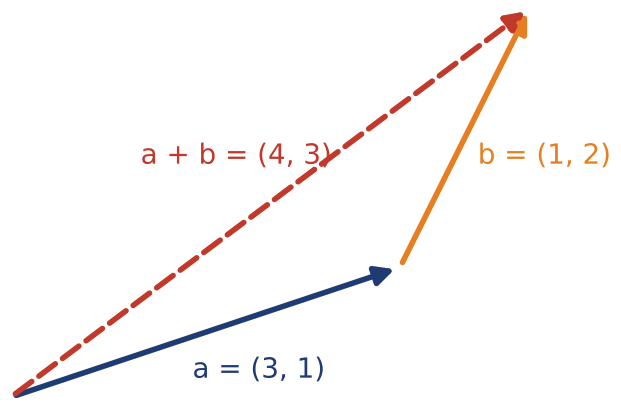
\includegraphics[width=\linewidth]{vectors}
\end{minipage}

\begin{eng}
A 3-D vector is written $\vect{v}=(v_x,v_y,v_z)^\mathsf{T}$. Vectors add component by component. Its length (norm) is $\|\vect{v}\|=\sqrt{v_x^2+v_y^2+v_z^2}$. Two products appear later:
\[ \vect{a}\cdot\vect{b}=a_xb_x+a_yb_y+a_zb_z \quad(\text{dot: a number}),\qquad
\vect{a}\times\vect{b}=\begin{pmatrix}a_yb_z-a_zb_y\\ a_zb_x-a_xb_z\\ a_xb_y-a_yb_x\end{pmatrix}\quad(\text{cross: a vector}). \]
The dot product measures how much two arrows point the same way. The cross product is perpendicular to both, and its length equals the area of the parallelogram they span --- which is why LIO-SAM uses it to measure distances to lines and planes (Module 11).
\end{eng}

\begin{worked}{dot and cross products}
\textbf{Given:} $\vect{a}=(1,2,0)$, $\vect{b}=(3,0,0)$.
\step{Dot} $1\cdot3+2\cdot0+0\cdot0 = 3$
\step{Cross} $(2\cdot0-0\cdot0,\ 0\cdot3-1\cdot0,\ 1\cdot0-2\cdot3)=(0,0,-6)$
\step{Meaning} The parallelogram spanned by $\vect a$ and $\vect b$ has area $\|(0,0,-6)\|=6$; with base $\|\vect b\|=3$ its height is $6/3=2$ --- exactly the distance from the tip of $\vect a$ to the line along $\vect b$.
\result{dot = 3, cross = (0, 0, $-$6), point-to-line distance = 2.}
\end{worked}

\section{Matrices in one page}
\begin{eng}
A matrix is a table of numbers that transforms a vector. Multiplying a $3\times3$ matrix by a vector gives a new vector whose each entry is a row of the matrix ``dotted'' with the vector:
\[\begin{pmatrix}a&b&c\\d&e&f\\g&h&i\end{pmatrix}\begin{pmatrix}x\\y\\z\end{pmatrix}=\begin{pmatrix}ax+by+cz\\dx+ey+fz\\gx+hy+iz\end{pmatrix}.\]
Key facts used later: the \textbf{transpose} $\vect{A}^\mathsf{T}$ swaps rows and columns; the \textbf{identity} $\vect I$ changes nothing; the \textbf{inverse} $\vect A^{-1}$ undoes $\vect A$; for a \emph{rotation} matrix the inverse is simply the transpose, $\vect R^{-1}=\vect R^\mathsf{T}$.
\end{eng}

\begin{worked}{matrix times vector}
$\begin{pmatrix}2&0&1\\0&1&0\\1&0&3\end{pmatrix}\begin{pmatrix}1\\4\\2\end{pmatrix}
=\begin{pmatrix}2\cdot1+0\cdot4+1\cdot2\\0\cdot1+1\cdot4+0\cdot2\\1\cdot1+0\cdot4+3\cdot2\end{pmatrix}=\begin{pmatrix}4\\4\\7\end{pmatrix}$
\end{worked}

\section{Statistics: mean, standard deviation, RMSE}
\fig[0.75]{gaussian}{Random measurement errors usually follow a bell curve. About 68\% fall within one standard deviation $\sigma$ and 95\% within 1.96$\sigma$.}

\begin{kid}
Throw ten paper balls at a target. The \textbf{mean} tells you where they landed on average (are you aiming too far left?). The \textbf{spread} (standard deviation) tells you how scattered they are. A great thrower has a mean right on the bullseye \emph{and} a small spread.
\end{kid}

\begin{keyeq}{Mean, standard deviation, RMSE}
\[ \bar e=\frac1n\sum_{i=1}^{n}e_i,\qquad
s=\sqrt{\frac{1}{n-1}\sum_{i=1}^{n}(e_i-\bar e)^2},\qquad
\text{RMSE}=\sqrt{\frac1n\sum_{i=1}^{n}e_i^2} \]
\begin{symbols}
$e_i$ & the $i$-th error (measured minus true) & m\\
$n$ & how many errors we have & ---\\
$\sum$ & ``add them all up,'' from $i=1$ to $n$ & ---\\
$\bar e$ & mean error = \emph{bias} (systematic part) & m\\
$s$ & sample standard deviation = \emph{precision} (random part); $n-1$ because one degree of freedom was spent computing $\bar e$ & m\\
RMSE & root-mean-square error = total \emph{accuracy}; combines bias and spread: $\text{RMSE}^2\approx\bar e^2+s^2$ & m\\
\end{symbols}
\end{keyeq}

\begin{worked}{five elevation errors}
\textbf{Given:} errors $+2, -1, +3, 0, +1$ cm.
\step{Mean} $(2-1+3+0+1)/5 = 5/5 = 1.0$ cm (a 1 cm high bias)
\step{Deviations from mean} $1,-2,2,-1,0$; squares $1,4,4,1,0$; sum $=10$
\step{Std.\ dev.} $s=\sqrt{10/4}=\sqrt{2.5}=1.58$ cm
\step{RMSE} squares of errors $4,1,9,0,1$; sum $=15$; RMSE $=\sqrt{15/5}=\sqrt3=1.73$ cm
\step{Check} $\bar e^2+s^2\cdot\tfrac{n-1}{n}=1+2.5\times0.8=3.0=\text{RMSE}^2$ \checkmark
\result{bias 1.0 cm, precision 1.58 cm, accuracy (RMSE) 1.73 cm.}
\end{worked}

\section{Adding independent errors: root-sum-square}
\begin{keyeq}{Propagation of independent errors}
\[ \sigma_{\text{total}}=\sqrt{\sigma_1^2+\sigma_2^2+\cdots+\sigma_k^2} \]
\begin{symbols}
$\sigma_j$ & standard deviation of the $j$-th independent error source & m\\
$\sigma_{\text{total}}$ & standard deviation of their sum & m\\
\end{symbols}
\end{keyeq}
Errors do \emph{not} add like ordinary numbers because random errors partly cancel. Two independent 3 cm and 4 cm errors combine to $\sqrt{9+16}=5$ cm, not 7 cm. The rule only holds when the sources are \emph{independent}; a systematic error that pushes every point the same way must be treated separately (see Module 13).

\begin{tryit}
\textbf{2.1} Convert 0.05° to radians, then find the sideways error it causes at 80 m.\\
\textbf{2.2} Compute $\sqrt{2^2+1.5^2+3^2}$.\\
\textbf{2.3} A wall is 12 m across and 5 m up from you along the slope. How long is the slope distance?\\
\textbf{2.4} (Simple) You need 3 big steps forward and then 4 big steps to the right. If you could walk straight there instead, how many steps would it be?
\end{tryit}

\sources{Ghilani, C.\ D.\ (2017), \emph{Adjustment Computations: Spatial Data Analysis}, 6th ed., Wiley (statistics, RMSE, propagation); NIST SP 811, \emph{Guide for the Use of the International System of Units}.}

\chapter{Measuring Distance with Light}

\section{Time of flight}
\fig[0.85]{tof}{A pulse travels out to the wall and back. The clock measures the whole round trip.}

\begin{kid}
Light is the fastest thing there is. In the time it takes you to blink, light could go around the world more than 2 times! The LiDAR starts a stopwatch when it flashes, and stops it when the flash bounces back. Because the light went \emph{to} the wall and \emph{back}, the wall is only half as far as the light traveled. So we cut the answer in half.
\end{kid}

\begin{keyeq}{Time-of-flight range}
\[ \rho=\frac{c\,\Delta t}{2},\qquad c=\frac{c_0}{n} \]
\begin{symbols}
$\rho$ & range (one-way distance from sensor to surface). Greek ``rho.'' & m\\
$\Delta t$ & measured round-trip time of flight & s\\
$c$ & speed of light \emph{in air} & m/s\\
$c_0$ & speed of light in vacuum, exactly 299\,792\,458 & m/s\\
$n$ & refractive index of air, about 1.0003 at sea level (depends on temperature, pressure, humidity) & ---\\
2 & the light travels the distance twice (out and back) & ---\\
\end{symbols}
\end{keyeq}

\begin{worked}{range from a 400 ns echo}
\textbf{Given:} $\Delta t = 400$ ns; standard air with $n=1.000300$.
\step{Step 1 --- speed of light in air} $c = 299\,792\,458/1.000300 = 299\,702\,547$ m/s
\step{Step 2 --- time in seconds} $400\text{ ns}=400\times10^{-9}=4.00\times10^{-7}$ s
\step{Step 3 --- round-trip path} $c\,\Delta t = 299\,702\,547\times4.00\times10^{-7}=119.881$ m
\step{Step 4 --- halve it} $\rho=119.881/2 = 59.941$ m
\result{$\rho\approx59.94$ m.}
\end{worked}

\begin{improve}
The seminar used $c\approx2.997\times10^8$ m/s and got 59.94 m. That value is right, but the reason matters: it is the \emph{vacuum} speed (2.9979$\times10^8$) divided by the refractive index of air. Using the vacuum value instead would give 59.958 m --- an 18 mm difference at 60 m, i.e.\ about 300 parts per million. Survey-grade processing applies an atmospheric correction for this, exactly as you set temperature and pressure on a total station's EDM.
\end{improve}

\section{How precise must the clock be?}
Rearranging the key equation for a small timing error $\delta t$:
\begin{keyeq}{Range error from timing error}
\[ \delta\rho = \frac{c\,\delta t}{2} \approx 0.15\ \text{m per nanosecond} \]
\begin{symbols}
$\delta\rho$ & error in the computed range & m\\
$\delta t$ & error in the measured time of flight & s\\
\end{symbols}
\end{keyeq}
\fig[0.72]{timing_error}{Range error grows in a straight line with timing error.}

So a 1 ns timing error ruins the range by 15 cm, and \emph{millimeter} ranging needs timing to about 7 picoseconds. Real sensors do not count clock ticks that finely; they digitize the returning pulse shape and interpolate its center, which is why waveform quality and signal strength matter so much.

\begin{tryit}
\textbf{3.1} An echo returns after 166.8 ns. What is the range (use $c=2.997\times10^8$ m/s)?\\
\textbf{3.2} What timing precision is needed for 1 cm range precision?
\end{tryit}

\section{Pulse rate and range ambiguity}
\begin{kid}
Imagine shouting ``Hello!'' every second in a giant canyon. If an echo takes 3 seconds, you won't know which ``Hello'' it belongs to. A LiDAR has the same problem if it fires the next flash before the last echo has come home.
\end{kid}

\fig[0.85]{ambiguity}{If the pulse repetition interval is shorter than the round-trip time, echoes get mixed up.}

\begin{keyeq}{Maximum unambiguous range}
\[ \rho_{\max}=\frac{c}{2\,f_{\text{PRF}}} \]
\begin{symbols}
$\rho_{\max}$ & farthest range that can be measured without confusion & m\\
$f_{\text{PRF}}$ & pulse repetition frequency: pulses fired per second & Hz (1/s)\\
\end{symbols}
\end{keyeq}

\begin{worked}{how fast can we fire?}
\textbf{Given:} $f_{\text{PRF}}=1$ MHz $=10^6$ pulses/s, $c=2.997\times10^8$ m/s.
\step{Step 1} time between pulses $=1/10^6=1\ \mu$s
\step{Step 2} $\rho_{\max}=2.997\times10^8/(2\times10^6)=149.9$ m
\step{Step 3 --- double the rate} at 2 MHz, $\rho_{\max}=74.9$ m
\result{faster firing = denser points but a shorter safe range. Modern sensors use ``multiple pulses in the air'' (MPiA) coding to beat this limit.}
\end{worked}

\section{Phase-shift (continuous-wave) ranging}
Some scanners send a continuous light wave whose brightness is modulated, and measure how far the returning wave has slid relative to the outgoing one.
\fig[0.75]{phase}{The returned wave is shifted by a fraction of a wavelength.}

\begin{keyeq}{Phase-shift range}
\[ \rho=\frac{\lambda_m}{2}\left(N+\frac{\Delta\varphi}{2\pi}\right),\qquad \lambda_m=\frac{c}{f_m} \]
\begin{symbols}
$\lambda_m$ & modulation wavelength (not the laser color!) & m\\
$f_m$ & modulation frequency & Hz\\
$\Delta\varphi$ & measured phase difference & rad\\
$N$ & whole number of half-wavelengths (the ``ambiguity''); solved by using several frequencies & ---\\
\end{symbols}
\end{keyeq}

\begin{worked}{phase measurement}
\textbf{Given:} $f_m=10$ MHz, $\Delta\varphi=90^\circ$, $c=2.997\times10^8$ m/s, $N=0$.
\step{Step 1} $\lambda_m=2.997\times10^8/10^7=29.97$ m; half-wavelength $=14.985$ m
\step{Step 2} $\Delta\varphi/2\pi = 90/360=0.25$
\step{Step 3} $\rho=14.985\times0.25=3.746$ m
\result{3.746 m --- or 18.731 m, or 33.716 m\ldots\ (add multiples of 14.985 m). A second, lower frequency decides which.}
\end{worked}

This is the same principle as most total-station EDMs. Phase scanners are very precise at short range (terrestrial scanners), while pulsed time-of-flight dominates long-range and mobile systems.

\section{Multiple returns}
\fig[0.92]{multireturn}{One wide pulse can hit leaves, a branch and the ground. The receiver sees several peaks.}

\begin{eng}
Because the beam has a finite width (Module 4), one pulse can partially hit several surfaces at different ranges. A \emph{discrete-return} sensor reports the first, intermediate and last peaks; a \emph{full-waveform} sensor records the whole curve. Each return gets its own range from its own time, $\rho_k=c\,t_k/2$. Last returns are the ones most likely to reach bare ground under vegetation --- the basis of terrain models in forests. Two surfaces closer together than about $c\,\tau/2$ (with $\tau$ the pulse width, e.g.\ 4 ns $\to$ 0.6 m) merge into a single peak.
\end{eng}

\begin{tip}
Edges of poles, curbs and building corners produce ``mixed pixels'': part of the beam hits the near object and part the far background, and the reported range can land in empty air between them. These show up as ghost points trailing behind edges and are removed in cleaning (Module 18).
\end{tip}

\sources{BIPM, \emph{The International System of Units} (speed of light $c_0=299\,792\,458$ m/s, exact); Ciddor, P.\ E.\ (1996), refractive index of air, \emph{Applied Optics} 35(9); Baltsavias, E.\ P.\ (1999), Airborne laser scanning: basic relations and formulas, \emph{ISPRS J.\ Photogramm.\ Remote Sens.} 54; RIEGL VUX-240\textsuperscript{24} datasheet (MTA processing).}

\chapter{The Laser Beam and the Echo}

\section{The beam spreads out}
\begin{kid}
Shine a flashlight at your hand: you see a small circle. Now shine it at a wall across the room: the circle is much bigger. A laser beam spreads too --- just very, very slowly. Far away, the laser ``dot'' can be as big as a coin, so it can touch the edge of a pole and the wall behind it at the same time.
\end{kid}

\fig[0.82]{footprint}{The footprint of a beam with 5 mm exit diameter and 0.3 mrad divergence.}

\begin{keyeq}{Beam footprint}
\[ D(\rho)\approx d_0+\rho\,\gamma \]
\begin{symbols}
$D$ & diameter of the laser spot on the target & m\\
$d_0$ & diameter of the beam as it leaves the sensor & m\\
$\rho$ & range & m\\
$\gamma$ & full-angle beam divergence (small-angle rule again!) & rad (often given in mrad = $10^{-3}$ rad)\\
\end{symbols}
\end{keyeq}

\begin{worked}{spot size at 50 m and 100 m}
\textbf{Given:} $d_0=5$ mm $=0.005$ m, $\gamma=0.3$ mrad $=0.0003$ rad.
\step{At 50 m} $D=0.005+50\times0.0003=0.005+0.015=0.020$ m $=2.0$ cm
\step{At 100 m} $D=0.005+100\times0.0003=0.035$ m $=3.5$ cm
\result{a 2--3.5 cm ``blur'' at mapping ranges. You cannot locate an edge more sharply than about half the spot size.}
\end{worked}

\section{How strong is the echo? The LiDAR range equation}
\begin{kid}
The farther away something is, the dimmer its echo. It gets dim fast: twice as far means only one quarter as bright. Shiny white things (a road sign) send back lots of light; black asphalt or wet surfaces send back very little. And if the light hits a surface at a slant, most of it bounces away like a ball skipping off water.
\end{kid}

\begin{keyeq}{Received power for an extended diffuse target}
\[ P_r = P_t\,\frac{\rho_{\text{refl}}\,\cos\theta_i}{\pi\,R^2}\,A_r\,\eta_{\text{sys}}\,\eta_{\text{atm}}^2 \]
\begin{symbols}
$P_r$ & power arriving at the detector & W\\
$P_t$ & power transmitted in the pulse & W\\
$\rho_{\text{refl}}$ & target reflectance (0 = black, 1 = perfect white) & ---\\
$\theta_i$ & incidence angle between beam and surface normal & rad\\
$R$ & range & m\\
$A_r$ & area of the receiving lens & m$^2$\\
$\eta_{\text{sys}}$ & optical efficiency of the sensor & ---\\
$\eta_{\text{atm}}$ & one-way atmospheric transmission (squared: out and back) & ---\\
$\pi$ & comes from a diffuse (Lambertian) surface scattering into a half-sphere & ---\\
\end{symbols}
\end{keyeq}

\fig[0.95]{power}{Left: the $1/R^2$ law. Right: the $\cos\theta_i$ incidence-angle law.}

\begin{worked}{comparing two targets}
\textbf{Given:} Target A: white concrete ($\rho_{\text{refl}}=0.6$) at 10 m, head-on. Target B: asphalt ($\rho_{\text{refl}}=0.1$) at 50 m, hit at 60°. Everything else equal.
\step{Step 1 --- ratio} $\dfrac{P_B}{P_A}=\dfrac{0.1}{0.6}\times\dfrac{\cos60^\circ}{\cos0^\circ}\times\dfrac{10^2}{50^2}$
\step{Step 2} $=0.1667\times0.5\times0.04=0.00333$
\result{B returns about 1/300 of A's power. Weak echoes have noisier ranges, which is why range precision gets worse with distance and grazing angle --- and why road surfaces far from the vehicle are the noisiest part of a mobile scan.}
\end{worked}

\section{Intensity}
Every point carries an \textbf{intensity} value, a number related to $P_r$. Because of the $R^2$ and $\cos\theta_i$ effects, raw intensity of the same paint changes with range and angle; software can \emph{normalize} it. Intensity makes road markings, signs and retro-reflective targets jump out of the cloud, which is handy for extracting line work and for finding control targets.

\section{Wavelength and eye safety}
\begin{eng}
Most automotive and mobile scanners use \textbf{905 nm} (near-infrared, cheap silicon detectors) or \textbf{1550 nm} (absorbed by the eye's cornea and lens before reaching the retina, so far more power may be used eye-safely --- giving longer range). All survey scanners used in public must be \textbf{Class 1} eye-safe under IEC 60825-1. Water strongly absorbs 1550 nm, so wet surfaces and rain reduce returns more at that wavelength; green (532 nm) lasers are used for bathymetric LiDAR because green light penetrates water.
\end{eng}

\section{What can LiDAR see through?}
\begin{kid}
A laser is light, so it acts like a flashlight beam, not like X-ray vision. It cannot see \emph{through} a wall, a tree trunk, or the ground. It \emph{can} slip through holes --- the gaps between leaves, the openings in a fence --- and reach whatever is behind them. It passes through clear glass the way sunlight does. And it is stopped almost right away by water.
\end{kid}

\fig[1.0]{penetration}{The five situations every LiDAR user meets. Orange dots are recorded returns.}

\begin{center}\small
\renewcommand{\arraystretch}{1.2}
\begin{tabularx}{\linewidth}{>{\raggedright\arraybackslash}p{3.0cm}>{\raggedright\arraybackslash}p{2.2cm}X}\toprule
\textbf{Material or condition} & \textbf{Does the laser get through?} & \textbf{What you get and what to do}\\\midrule
Tree canopy, shrubs & \textbf{Through the gaps only} & First returns on leaves, last returns on the ground where there are openings. Dense evergreen or summer canopy may leave no ground hits: collect in leaf-off season, slow down, add passes.\\
Tall grass, crops, mangroves & \textbf{Rarely} & Points sit on top of the vegetation, not the soil. Heights are biased high; take ground shots by conventional methods.\\
Chain-link fence, mesh, railings & \textbf{Partly} (gaps) & Some points on the fence, some behind it; the fence appears as a sparse ghost surface.\\
Clear glass windows & \textbf{Mostly through} & Few returns from the glass itself (except head-on); you see the room behind. Reflections can create ``mirror-world'' ghost points.\\
Tinted, frosted or coated glass & \textbf{Partly / varies} & Unpredictable; check the cloud.\\
Mirrors, polished metal, chrome & \textbf{No --- reflects away} & Dropouts or ghost points placed at false ranges behind the surface.\\
Water (865--1550 nm) & \textbf{No} & Absorbed within centimeters; calm water often returns nothing except straight down. Only green (532 nm) bathymetric LiDAR maps the bottom, in clear water.\\
Wet pavement, puddles & \textbf{No} & Weak or missing returns; specular reflection; schedule collection after surfaces dry.\\
Rain, fog, dust, smoke, steam & \textbf{Partly} & Range shortens; ``floating'' false points near the sensor; heavy fog can block completely. Filter them out (Module 18).\\
Falling snow & \textbf{Partly} & Noise points in the air; snow cover hides the ground surface.\\
Walls, soil, pavement, people, vehicles & \textbf{No} & Opaque: anything behind is in shadow. Plan extra passes or positions to see behind objects.\\
Underground utilities & \textbf{No} & LiDAR maps only visible surfaces (manhole lids, valve covers). Use ground-penetrating radar or locating for what is buried.\\\bottomrule
\end{tabularx}\end{center}

\begin{bigidea}
LiDAR never ``penetrates'' solid material. It reaches hidden ground only through openings, which is why multiple returns (Module 3) and many viewing angles matter more than laser power.
\end{bigidea}

\section{Reflectivity of common surfaces}
\fig[0.86]{reflectivity}{Typical reflectivity of common surfaces at the near-infrared wavelengths used by most mobile scanners (865--905 nm). Values vary with moisture, age, roughness, color and incidence angle.}

\begin{center}\small
\renewcommand{\arraystretch}{1.18}
\begin{tabularx}{\linewidth}{>{\raggedright\arraybackslash}p{4.2cm}>{\centering\arraybackslash}p{2.3cm}X}\toprule
\textbf{Surface} & \textbf{Typical reflectivity} & \textbf{What it means in the field}\\\midrule
Clear, calm water & 1--5\% & often no return at all except straight below the sensor\\
Black tire, rubber & 2--5\% & among the darkest targets; shortest detection range\\
Black or dark car paint & 3--8\% & cars may appear with holes; glossy paint can also mirror\\
Fresh asphalt & 4--8\% & dark: road returns thin out first at long range\\
Wet soil, wet asphalt & 4--12\% & water darkens surfaces in the near infrared\\
Dark rock (basalt) & 5--15\% & dark\\
Aged, gray asphalt & 10--20\% & brighter as it weathers\\
Dry soil & 15--35\% & medium\\
Tree bark, wood & 20--45\% & medium\\
Concrete & 25--50\% & good, consistent target\\
Dry sand & 30--55\% & bright\\
Grass, green leaves & 40--60\% & bright in the near infrared (healthy plants reflect strongly there)\\
White paint, road striping & 60--85\% & very bright: striping stands out in intensity images\\
Fresh snow & 75--95\% at 865--905 nm & very bright at 905 nm --- but much darker at 1550 nm\\
Retroreflective signs and tape & ``over 100\%'' & sends light straight back; can saturate the receiver and bias the range (Module 15)\\\bottomrule
\end{tabularx}\end{center}
{\footnotesize Values are typical ranges compiled for teaching; they are not specifications. Sensors that report \emph{calibrated reflectivity} (such as the Ouster OS0) let you measure your own surfaces.}

\begin{worked}{how far can I see dark asphalt?}
\textbf{Given:} the OS0 detects a 10\% target to 35 m (Module 15). Received power falls as $1/R^2$ (Section 4.2), so for the same detection threshold the maximum range grows as the \emph{square root} of reflectivity.
\step{Fresh asphalt, 5\%} $35\times\sqrt{5/10}=35\times0.71=25$ m
\step{Black car, 4\%} $35\times\sqrt{0.4}=22$ m
\step{Concrete, 40\%} $35\times\sqrt{4}=70$ m (the datasheet's 75 m at 80\% shows the rule flattening out in bright sunlight)
\result{plan the usable swath on the \emph{darkest} surface you must map: on new asphalt, expect road coverage to end near 25 m, long before the brochure range.}
\end{worked}

\section{Range precision in practice}
\begin{center}\small
\renewcommand{\arraystretch}{1.2}
\begin{tabularx}{\linewidth}{Xl}\toprule
\textbf{Situation} & \textbf{Typical range noise (1$\sigma$)}\\\midrule
Good mobile unit, bright hard target, under 30 m (100 ft) & 1--3 cm (0.03--0.10 ft)\\
Same unit, dark or grazing target, 50--100 m (165--330 ft) & 5--15 cm (0.16--0.49 ft)\\
Survey-grade mobile mapping head & 3--8 mm (0.01--0.03 ft)\\
Terrestrial phase scanner, short range & 1--3 mm (0.003--0.010 ft)\\\bottomrule
\end{tabularx}\end{center}
These are order-of-magnitude illustrations; always read the specification sheet and, more importantly, \emph{test on your own control}.

\begin{tryit}
\textbf{4.1} A beam has $d_0=8$ mm and $\gamma=0.5$ mrad. How wide is the spot at 40 m?\\
\textbf{4.2} By what factor does echo power drop when a target moves from 20 m to 60 m?\\
\textbf{4.3} (Simple) Which gives a brighter echo: a white sign or a black tire? Why?\\
\textbf{4.4} (Simple) Which of these can a mobile LiDAR measure the ground behind: a leafy tree, a brick wall, a glass storefront, a pond?
\end{tryit}

\sources{Baltsavias (1999), \emph{ISPRS J.} 54 (range equation, footprint); IEC 60825-1:2014 (laser classes); Ouster OS0 Rev8 datasheet (calibrated reflectivity, detection ranges at 10\% and 80\%); reflectivity values are typical teaching ranges --- measured spectra are available in the USGS Spectral Library Version 7 (Kokaly \emph{et al.}, 2017).}

\chapter{From Angles and Distance to X, Y, Z}

\section{The idea}
\begin{kid}
To tell a friend where a treasure is hidden, you could say: ``Face the big tree. Turn a little to the left. Look a little up. Now walk 25 steps that way.'' That is a \textbf{turn}, a \textbf{tilt} and a \textbf{distance}. A LiDAR records the same three things for every dot. Then it does some triangle math to change them into ``how far forward, how far sideways, how far up'' --- which we call X, Y and Z.
\end{kid}

\fig[0.6]{polar3d}{A range of 25 m with horizontal angle 40° and vertical angle 15° becomes a point at (18.50, 15.52, 6.47) m.}

\begin{keyeq}{Polar (spherical) to Cartesian}
\[ x_s=\rho\cos V\cos H,\qquad y_s=\rho\cos V\sin H,\qquad z_s=\rho\sin V \]
\begin{symbols}
$x_s,y_s,z_s$ & point coordinates in the \emph{sensor} frame (subscript $s$) & m\\
$\rho$ & measured range & m\\
$H$ & horizontal angle (azimuth in the sensor), measured from the sensor's $x$-axis toward its $y$-axis & deg/rad\\
$V$ & vertical angle above the sensor's horizontal plane (elevation). Note: a total station's \emph{zenith} angle $Z_a$ is $90^\circ-V$ & deg/rad\\
$\rho\cos V$ & the horizontal part of the range (its shadow on the floor) & m\\
\end{symbols}
\end{keyeq}

\begin{eng}
Read the equation in two moves. \textbf{First tilt:} the vertical angle splits the range into a horizontal part $\rho\cos V$ and a height $\rho\sin V$. \textbf{Then turn:} the horizontal angle splits the horizontal part into $x$ and $y$. That is why $\cos V$ appears in both $x$ and $y$. In a spinning scanner, $H$ comes from the motor's angle encoder at the instant of firing, and $V$ is the fixed elevation angle of the laser channel (``ring'') that fired. Conventions differ by manufacturer (some measure $H$ clockwise, some use zenith angles), so always check the sensor's documentation.
\end{eng}

\fig[0.95]{polar_steps}{The two moves: tilt (side view), then turn (top view).}

\begin{worked}{one laser return to sensor coordinates}
\textbf{Given:} $\rho=25.000$ m, $H=40.0^\circ$, $V=15.0^\circ$. Sensor frame: $x$ forward, $y$ left, $z$ up.
\step{Step 1 --- trig values} $\cos15^\circ=0.96593$, $\sin15^\circ=0.25882$, $\cos40^\circ=0.76604$, $\sin40^\circ=0.64279$
\step{Step 2 --- horizontal part} $\rho\cos V=25.000\times0.96593=24.148$ m
\step{Step 3 --- split it} $x_s=24.148\times0.76604=18.499$ m;\quad $y_s=24.148\times0.64279=15.522$ m
\step{Step 4 --- height} $z_s=25.000\times0.25882=6.470$ m
\step{Step 5 --- check} $\sqrt{18.499^2+15.522^2+6.470^2}=\sqrt{342.21+240.93+41.86}=\sqrt{625.00}=25.000$ \checkmark
\result{$(x_s,y_s,z_s)=(18.50,\ 15.52,\ 6.47)$ m.}
\end{worked}

\begin{improve}
The seminar used ``$Y$ right'' with a counter-clockwise $H$. Those two choices are inconsistent for a right-handed frame with $Z$ up: with $X$ forward and $Z$ up, a right-handed $Y$ points \emph{left}. We use the robotics standard (ROS REP-103: $x$ forward, $y$ left, $z$ up) throughout this course, and we added the length check in Step 5 --- a habit worth keeping: the computed coordinates must reproduce the measured range.
\end{improve}

\section{Going backward: Cartesian to polar}
\begin{keyeq}{Inverse conversion}
\[ \rho=\sqrt{x^2+y^2+z^2},\qquad H=\operatorname{atan2}(y,x),\qquad V=\operatorname{atan2}\!\left(z,\sqrt{x^2+y^2}\right) \]
\begin{symbols}
$\operatorname{atan2}(a,b)$ & the angle whose tangent is $a/b$, placed in the correct quadrant using the signs of $a$ and $b$ & rad\\
\end{symbols}
\end{keyeq}
This is what the SLAM software uses to \emph{predict} what range and bearing the sensor should see to a known object (Module 10).

\section{Mechanical versus solid-state scanners}
\fig[1.0]{patterns}{How three kinds of scanner sample the world (angles in degrees).}

\begin{center}\small
\renewcommand{\arraystretch}{1.2}
\begin{tabularx}{\linewidth}{lXX}\toprule
 & \textbf{Mechanical (spinning)} & \textbf{Solid-state}\\\midrule
How the beam moves & a motor spins a stack of 16--128 lasers & MEMS mirror, prisms (rosette), optical phased array, or flash (no motion)\\
Field of view & 360° horizontal, 30--90° vertical & typically 60--120° wide, forward-looking\\
Point pattern & regular rings & raster or non-repeating; coverage fills in over time\\
Strengths & full surround view, mature, well-modeled & small, light, rugged, cheap, no large moving parts\\
Watch-outs & motor wear, size, cost & narrower view; need several units or motion for full coverage; pattern-specific calibration\\\bottomrule
\end{tabularx}\end{center}

\section{How dense will my points be?}
\begin{kid}
Imagine painting a road with a paint-roller that only touches the road once every big step. If you walk faster, the stripes get further apart. If you roll faster, they get closer.
\end{kid}

\fig[0.85]{spacing}{Each sweep of the scanner lays a line of points across the road.}

\begin{keyeq}{Point spacing and point rate}
\[ \Delta_{\text{along}}=\frac{v}{f_{\text{rot}}},\qquad \Delta_{\text{across}}\approx\rho\,\Delta\theta,\qquad N_{\text{pts/s}}=N_{\text{ch}}\times N_{\text{az}}\times f_{\text{rot}} \]
\begin{symbols}
$\Delta_{\text{along}}$ & spacing between scan lines in the direction of travel & m\\
$v$ & platform speed & m/s\\
$f_{\text{rot}}$ & rotation (scan-line) rate & Hz\\
$\Delta_{\text{across}}$ & spacing between neighboring points along one scan line & m\\
$\Delta\theta$ & angular step between pulses & rad\\
$N_{\text{ch}}$ & number of laser channels & ---\\
$N_{\text{az}}$ & azimuth steps per revolution ($360^\circ/\Delta\theta$) & ---\\
\end{symbols}
\end{keyeq}

\begin{worked}{planning a corridor survey}
\textbf{Given:} 16-channel scanner, 0.2° horizontal step, 10 Hz, driving 15 m/s (54 km/h). Target 20 m away.
\step{Step 1 --- along-track} $\Delta_{\text{along}}=15/10=1.5$ m between sweeps (for each channel)
\step{Step 2 --- across-track} $0.2^\circ=0.003491$ rad; $\Delta_{\text{across}}=20\times0.003491=0.070$ m
\step{Step 3 --- point rate} $N_{\text{az}}=360/0.2=1800$; $N=16\times1800\times10=288\,000$ points/s
\step{Step 4 --- slow down} at 5 m/s the along-track spacing becomes 0.5 m
\result{1.5 m between lines is fine for a pavement surface but too coarse for curb lines or small utilities --- drive slower, tilt the scanner, or use more channels.}
\end{worked}

\begin{tip}
Mobile mapping heads for survey work are often mounted \emph{tilted} so the spinning plane slices the road at an angle; then several channels hit the same strip of road at different times and along-track gaps close up. Point-density specifications should be checked on the delivered data (points per m$^2$ on a test patch), not assumed from the brochure.
\end{tip}

\begin{tryit}
\textbf{5.1} Convert $\rho=40.000$ m, $H=-30^\circ$, $V=5^\circ$ into $(x_s,y_s,z_s)$. Check the length.\\
\textbf{5.2} A point is at $(3.0,\,4.0,\,12.0)$ m in the sensor frame. Find $\rho$, $H$ and $V$.\\
\textbf{5.3} A 32-channel scanner spins at 20 Hz with 0.4° steps. How many points per second? What is the along-track spacing at 10 m/s?
\end{tryit}

\sources{ROS REP-103, \emph{Standard Units of Measure and Coordinate Conventions}; Ouster OS0 Rev8 datasheet (channels, columns, field of view).}

\chapter{Rotation, Pose and Frames}

\section{Pose = where you are + which way you face}
\begin{kid}
Stand in the middle of a room. ``Where you are'' is your spot on the floor (and how tall you are). ``Which way you face'' is whether you look at the board or the window, whether you tilt your head, whether you lean. A LiDAR on a car needs to know both of these things, all the time, because the car bumps, turns and leans. Together they are called its \textbf{pose}.
\end{kid}

\begin{eng}
Pose has six degrees of freedom: position $\vect p=(X,Y,Z)$ and orientation, usually written as three angles --- \textbf{roll} $\phi$, \textbf{pitch} $\theta$, \textbf{yaw} $\psi$ --- or as a $3\times3$ rotation matrix $\vect R$, or a unit quaternion. In LIO-SAM's notation the pose is a rigid-body transformation $\vect T=[\vect R\mid\vect p]\in SE(3)$, where $SE(3)$ (``special Euclidean group'') is simply the set of all rotations-plus-translations, and $\vect R\in SO(3)$ (``special orthogonal group'') the set of all proper rotation matrices.
\end{eng}

\fig[0.95]{rpy}{Roll, pitch and yaw on a mapping vehicle.}

\begin{center}\small
\renewcommand{\arraystretch}{1.2}
\begin{tabularx}{\linewidth}{lllX}\toprule
\textbf{Angle} & \textbf{About axis} & \textbf{Everyday example} & \textbf{Effect of a residual error on the map}\\\midrule
Roll $\phi$ & $x$ (forward) & banked curve & tilts points left/right of the drive line; heights wrong on one side\\
Pitch $\theta$ & $y$ (sideways) & climbing a grade & far points too high/low ahead of and behind the vehicle\\
Yaw $\psi$ & $z$ (vertical) & turning a corner & rotates the whole scan; lateral error grows with range\\\bottomrule
\end{tabularx}\end{center}

\section{The right-hand rule: naming X, Y, Z and roll, pitch, yaw}
\begin{kid}
Hold up your \textbf{right} hand. Point your \textbf{first (index) finger} straight ahead --- that is \textbf{X}. Point your \textbf{middle finger} to the left --- that is \textbf{Y}. Stick your \textbf{thumb} straight up --- that is \textbf{Z}. \textbf{The thumb is always Z.} Another way to say it: curl your fingers from X toward Y, and your thumb points to Z. Now make a thumbs-up: the way your curled fingers wrap around your thumb is the ``plus'' direction for turning around that thumb. Point your thumb along X and your fingers show plus \textbf{roll}; along Y, plus \textbf{pitch}; along Z (straight up), plus \textbf{yaw}.
\end{kid}

\fig[1.0]{righthand}{The right-hand rule. Left: index finger = X, middle finger = Y, and the thumb is always Z; equivalently, the fingers curl from X toward Y and the thumb points to Z. Right: with the thumb along an axis, the curled fingers show the positive rotation about it --- roll about X, pitch about Y, yaw about Z.}

\begin{eng}
\textbf{Rule 1 --- the axes form a right-handed set.} With the right hand: index finger $=+X$, middle finger $=+Y$, \textbf{thumb $=+Z$} --- the thumb is always Z. Equivalently, curl the fingers from $+X$ toward $+Y$ and the thumb points along $+Z$; mathematically $\hat{\vect x}\times\hat{\vect y}=\hat{\vect z}$ (Module 2). (Some textbooks label the fingers in a different order, e.g.\ thumb $=X$; any cyclic relabeling gives the same right-handed set, but this course keeps the thumb on Z throughout so that axis naming and the rotation rule below use the hand the same way.) Every coordinate frame in this course --- sensor, body, IMU, world (ENU) and map projection with height --- is right-handed. A left-handed frame (one axis flipped) is a mirror image, and no rotation can turn one into the other; mixing them is a classic cause of a ``mirrored'' point cloud.

\textbf{Rule 2 --- positive rotations follow the curl.} Point the right thumb along the positive axis; the fingers curl in the direction of a \emph{positive} angle. Seen from the arrow tip looking back toward the origin, positive is \textbf{counter-clockwise}.
\begin{itemize}
\item \textbf{Roll} $\phi$ = rotation about $+X$
\item \textbf{Pitch} $\theta$ = rotation about $+Y$
\item \textbf{Yaw} $\psi$ = rotation about $+Z$
\end{itemize}
Because the \emph{direction} of each axis decides the sign, the same physical motion can be $+$ in one convention and $-$ in another. The two conventions you will meet most:
\end{eng}

\fig[0.95]{rhr_vehicle}{The same vehicle in the two common right-handed body frames.}

\begin{center}\small
\renewcommand{\arraystretch}{1.25}
\begin{tabularx}{\linewidth}{>{\bfseries}p{2.2cm}XX}\toprule
 & FLU: X forward, Y left, Z up & FRD: X forward, Y right, Z down\\\midrule
Used by & ROS (REP-103), LIO-SAM, most LiDAR drivers, this course & aircraft, many INS/IMU products (NED world frame)\\
+ roll (about X) & left side \emph{up}, right side down & right side \emph{down}\\
+ pitch (about Y) & nose \emph{down} & nose \emph{up}\\
+ yaw (about Z) & nose turns \emph{left} (counter-clockwise from above) & nose turns \emph{right} (clockwise from above, like azimuth)\\
World frame & ENU: East, North, Up & NED: North, East, Down\\\bottomrule
\end{tabularx}\end{center}

\begin{worked}{checking a frame with your hand (and with the cross product)}
\textbf{Given:} a datasheet says a sensor's axes are ``X forward, Y right, Z up.''
\step{Hand test} right index finger forward (X), middle finger right (Y) --- the thumb (Z) now points \emph{down}, not up.
\step{Cross-product test} forward $\times$ right $=(1,0,0)\times(0,-1,0)=(0,0,-1)$ = down in a frame where $(0,1,0)$ is left.
\result{``X forward, Y right, Z up'' is \textbf{left-handed}. Either the datasheet means Z down (FRD) or one axis is mislabeled. Resolve it with the manufacturer before computing a single lever arm or boresight; a sign error here mirrors or tilts the entire cloud.}
\end{worked}

\begin{tip}
When setting up a rig, stand behind the vehicle, hold up your right hand in the way the manual defines the axes, and \emph{physically} roll, pitch and yaw the IMU a few degrees while watching the live output. Each angle should increase in the direction your fingers curl. Write the verified convention in the calibration record (Appendix E).
\end{tip}

\section{Rotating a point in 2-D}
\fig[0.42]{rot2d}{Rotating $\vect p=(3,4)$ by 30° counter-clockwise.}

\begin{keyeq}{2-D rotation}
\[ \begin{pmatrix}x'\\y'\end{pmatrix}=\underbrace{\begin{pmatrix}\cos\psi&-\sin\psi\\\sin\psi&\cos\psi\end{pmatrix}}_{\vect R(\psi)}\begin{pmatrix}x\\y\end{pmatrix} \]
\begin{symbols}
$(x,y)$ & original point & m\\
$(x',y')$ & point after rotation & m\\
$\psi$ & rotation angle, positive counter-clockwise (``psi'') & rad\\
$\vect R(\psi)$ & the rotation matrix; its columns are where the $x$- and $y$-axes end up & ---\\
\end{symbols}
\end{keyeq}

\begin{worked}{rotate (3, 4) by 30°}
\step{Step 1} $\cos30^\circ=0.86603$, $\sin30^\circ=0.50000$
\step{Step 2} $x'=0.86603\times3-0.5\times4=2.59808-2.00000=0.598$
\step{Step 3} $y'=0.5\times3+0.86603\times4=1.50000+3.46410=4.964$
\step{Step 4 --- check} length before $=\sqrt{9+16}=5$; after $=\sqrt{0.598^2+4.964^2}=\sqrt{0.358+24.642}=5.000$ \checkmark
\result{$(0.598,\ 4.964)$. A rotation never changes lengths --- a great error check.}
\end{worked}

\section{Rotations in 3-D}
\begin{keyeq}{The three elementary rotations}
\[ \vect R_x(\phi)=\begin{pmatrix}1&0&0\\0&\cos\phi&-\sin\phi\\0&\sin\phi&\cos\phi\end{pmatrix}\!,\
\vect R_y(\theta)=\begin{pmatrix}\cos\theta&0&\sin\theta\\0&1&0\\-\sin\theta&0&\cos\theta\end{pmatrix}\!,\
\vect R_z(\psi)=\begin{pmatrix}\cos\psi&-\sin\psi&0\\\sin\psi&\cos\psi&0\\0&0&1\end{pmatrix} \]
\[ \vect R=\vect R_z(\psi)\,\vect R_y(\theta)\,\vect R_x(\phi) \qquad(\text{``ZYX'' or yaw--pitch--roll order}) \]
\begin{symbols}
$\phi,\theta,\psi$ & roll, pitch, yaw (``phi, theta, psi'') & rad\\
$\vect R_x$ etc. & rotation about one axis only; the axis's own row and column hold 1 and 0s & ---\\
$\vect R$ & the full body-to-world rotation; applied right-to-left: roll first, then pitch, then yaw & ---\\
\end{symbols}
\end{keyeq}

\begin{eng}
\textbf{Order matters.} Rotating 90° about $x$ then 90° about $z$ ends somewhere different than the reverse order --- try it with a book. Every software package documents its order and sign convention; a large share of real-world georeferencing bugs are convention mismatches. Two other important facts:
\begin{itemize}
\item $\vect R^\mathsf{T}\vect R=\vect I$ and $\det\vect R=+1$. So the inverse rotation (world-to-body) is just $\vect R^\mathsf{T}$. LIO-SAM writes $\vect R_t=\vect R^{\mathsf{WB}}_t={\vect R^{\mathsf{BW}}_t}^{\mathsf T}$ for exactly this reason.
\item In the FLU frame used here ($x$ forward, $y$ left, $z$ up), a \emph{positive} rotation about $y$ tips the nose \emph{down}. Many INS products use FRD ($x$ forward, $y$ right, $z$ down) where positive pitch is nose up. Always confirm.
\end{itemize}
\end{eng}

\begin{tip}
\textbf{Yaw is not azimuth.} Surveyors measure azimuth clockwise from grid north. ROS/ENU systems measure yaw counter-clockwise from east. Convert with $\psi=90^\circ-\alpha_{\text{az}}$. A vehicle heading due north has $\alpha_{\text{az}}=0^\circ$ but $\psi=90^\circ$. Grid north also differs from true north by the \emph{convergence angle} of your map projection --- another place a heading can quietly go wrong.
\end{tip}

\section{Homogeneous transforms: rotation and shift in one matrix}
\begin{keyeq}{Rigid-body transformation}
\[ \vect r_W=\vect R\,\vect r_B+\vect p
\quad\Longleftrightarrow\quad
\begin{pmatrix}\vect r_W\\1\end{pmatrix}=\underbrace{\begin{pmatrix}\vect R&\vect p\\\vect 0^{\mathsf T}&1\end{pmatrix}}_{\vect T}\begin{pmatrix}\vect r_B\\1\end{pmatrix} \]
\begin{symbols}
$\vect r_B$ & a point expressed in the body (vehicle/IMU) frame B & m\\
$\vect r_W$ & the same point expressed in the world frame W & m\\
$\vect R$ & body-to-world rotation & ---\\
$\vect p$ & position of the body origin in W & m\\
$\vect T$ & $4\times4$ transform; chaining frames = multiplying $\vect T$'s & ---\\
\end{symbols}
\end{keyeq}
The relative motion between two poses is $\Delta\vect T_{i,j}=\vect T_i^{-1}\vect T_j$. That is LIO-SAM's equation (12), which defines the \emph{lidar odometry factor} (Module 12). (The paper prints it as $\vect T_i^{\mathsf T}\vect T_{i+1}$; for the full $4\times4$ matrix the correct operation is the inverse, which equals the transpose only for the rotation block.)

\section{Rotation from a turning rate: the exponential map}
Gyroscopes give angular \emph{rates}. Over a short time $\Delta t$ the body turns through a rotation vector $\boldsymbol\omega\Delta t$ (direction = axis, length = angle). LIO-SAM's equation (6) converts that small turn into a rotation matrix with the exponential map:
\begin{keyeq}{Rotation update (Rodrigues' formula)}
\[ \vect R_{t+\Delta t}=\vect R_t\exp\!\big([\boldsymbol\omega\Delta t]_\times\big),\qquad
\exp([\vect a]_\times)=\vect I+\frac{\sin\alpha}{\alpha}[\vect a]_\times+\frac{1-\cos\alpha}{\alpha^2}[\vect a]_\times^2 \]
\begin{symbols}
$\boldsymbol\omega$ & angular-rate vector from the gyros (bias-corrected) & rad/s\\
$\vect a$ & rotation vector $\boldsymbol\omega\Delta t$; $\alpha=\|\vect a\|$ is the turn angle & rad\\
$[\vect a]_\times$ & skew-symmetric matrix $\begin{psmallmatrix}0&-a_z&a_y\\a_z&0&-a_x\\-a_y&a_x&0\end{psmallmatrix}$; $[\vect a]_\times\vect b=\vect a\times\vect b$ & rad\\
\end{symbols}
\end{keyeq}

\begin{worked}{one gyro step}
\textbf{Given:} yaw rate $\omega_z=0.0842$ rad/s (from a real IMU message in the seminar), $\Delta t=0.005$ s (200 Hz). Start level, heading $\psi=0$.
\step{Step 1} $\alpha=0.0842\times0.005=0.000421$ rad $=0.0241^\circ$, all about $z$
\step{Step 2} For rotation purely about $z$, Rodrigues reduces to $\vect R_z(\alpha)$: $\cos\alpha=0.99999991$, $\sin\alpha=0.000421$
\step{Step 3} New heading $\psi=0.0241^\circ$. If the rate stays constant, 200 such steps (1 s) add up to $200\times0.000421=0.0842$ rad $=4.82^\circ$
\result{the strapdown computer repeats this tiny multiplication 200 times per second to track attitude.}
\end{worked}

\section{Why tiny angle errors matter}
\fig[0.72]{smallangle}{Lateral error versus range for three residual angle errors.}

\begin{worked}{0.05° heading error at 80 m}
\step{Step 1 --- radians} $0.05\times\pi/180=0.0008727$ rad
\step{Step 2 --- small-angle rule} $80\times0.0008727=0.0698$ m
\result{7.0 cm. At 100 m: 8.7 cm. A 0.1° error at 100 m: 17.5 cm --- bigger than most engineering tolerances.}
\end{worked}

\begin{tryit}
\textbf{6.1} Rotate $(10,0)$ by $90^\circ$; then rotate $(0,10)$ by $-90^\circ$. What do you notice?\\
\textbf{6.2} A vehicle drives with azimuth 135° (southeast). What is its ENU yaw?\\
\textbf{6.3} What heading error produces 2 cm lateral error at 40 m?
\end{tryit}

\sources{ROS REP-103 (FLU body frame, ENU world frame); Groves, P.\ D.\ (2013), \emph{Principles of GNSS, Inertial, and Multisensor Integrated Navigation Systems}, 2nd ed.\ (rotations, FRD/NED conventions); Shan \emph{et al.}\ (2020), eq.\ (6), (12).}

\chapter{The IMU: Feeling Motion}

\section{What is inside an IMU?}
\begin{kid}
When a car speeds up, you get pushed back into your seat. When it turns, you lean to the side. Your body \emph{feels} the motion even with your eyes closed. An IMU is a little box that feels motion the same way. It has three ``push-feelers'' (accelerometers) --- forward, sideways, up --- and three ``spin-feelers'' (gyroscopes). By adding up all those feelings many times a second, the computer can guess where the car went, even inside a tunnel. But like walking with your eyes closed, the guess slowly gets worse.
\end{kid}

\fig[0.92]{imuparts}{An accelerometer is a mass on springs; a gyroscope senses turning rate.}

\begin{eng}
An \textbf{inertial measurement unit} contains a triad of accelerometers measuring \emph{specific force} $\vect f$ (acceleration minus gravity) and a triad of gyroscopes measuring \emph{angular rate} $\boldsymbol\omega$, both in the body frame, typically at 100--1000 Hz. The sensors are rigidly fixed (``strapped down'') to the platform; the computer --- not a gimbal --- keeps track of orientation. An at-rest, level accelerometer reads $+9.81$ m/s$^2$ upward (it feels the table pushing up), which is why an IMU message at rest shows $a_z\approx9.78$--$9.81$.
\end{eng}

\section{The IMU measurement model (LIO-SAM eqs.\ 2--3)}
\begin{keyeq}{What the IMU actually reports}
\[ \hat{\boldsymbol\omega}_t=\boldsymbol\omega_t+\vect b^{\omega}_t+\vect n^{\omega}_t \qquad\qquad
\hat{\vect a}_t=\vect R^{\mathsf{BW}}_t(\vect a_t-\vect g)+\vect b^{a}_t+\vect n^{a}_t \]
\begin{symbols}
$\hat{\boldsymbol\omega}_t,\ \hat{\vect a}_t$ & raw gyro and accelerometer readings at time $t$ (the ``hat'' means \emph{measured}) & rad/s, m/s$^2$\\
$\boldsymbol\omega_t$ & the true angular rate of the body & rad/s\\
$\vect a_t$ & the true acceleration of the body, in the world frame W & m/s$^2$\\
$\vect g$ & gravity vector in W, about $(0,0,-9.81)$ & m/s$^2$\\
$\vect R^{\mathsf{BW}}_t$ & rotation from world to body: expresses the world vector in sensor axes & ---\\
$\vect b^{\omega}_t,\vect b^{a}_t$ & \textbf{biases}: slowly drifting offsets (the big villains) & rad/s, m/s$^2$\\
$\vect n^{\omega}_t,\vect n^{a}_t$ & white noise: fast random jitter & rad/s, m/s$^2$\\
\end{symbols}
\end{keyeq}
In words: \emph{reading = truth + slow offset + fast jitter}. Note the accelerometer equation: subtracting $\vect g$ (which points down) \emph{adds} 9.81 upward --- that is the ``table pushing up'' reading at rest.

\section{Strapdown integration (LIO-SAM eqs.\ 4--6)}
\fig[0.78]{integrate}{Acceleration is summed into velocity; velocity is summed into position.}

\begin{keyeq}{Dead-reckoning update over one IMU interval}
\begin{align*}
\vect v_{t+\Delta t}&=\vect v_t+\vect g\Delta t+\vect R_t(\hat{\vect a}_t-\vect b^a_t-\vect n^a_t)\Delta t\\
\vect p_{t+\Delta t}&=\vect p_t+\vect v_t\Delta t+\tfrac12\vect g\Delta t^2+\tfrac12\vect R_t(\hat{\vect a}_t-\vect b^a_t-\vect n^a_t)\Delta t^2\\
\vect R_{t+\Delta t}&=\vect R_t\exp\!\big((\hat{\boldsymbol\omega}_t-\vect b^{\omega}_t-\vect n^{\omega}_t)\Delta t\big)
\end{align*}
\begin{symbols}
$\vect v_t,\vect p_t$ & velocity and position of the body in W & m/s, m\\
$\vect R_t$ & body-to-world rotation (attitude) at time $t$ & ---\\
$\Delta t$ & IMU sample interval (0.01 s at 100 Hz) & s\\
$\hat{\vect a}_t-\vect b^a_t$ & the bias-corrected accelerometer reading (noise unknown, treated as zero mean) & m/s$^2$\\
$\vect R_t(\cdot)$ & rotates the body-frame reading into world axes & ---\\
$\vect g\Delta t$ & puts gravity back so a sensor at rest does not ``fly upward'' & m/s\\
$\tfrac12(\cdot)\Delta t^2$ & the familiar $s=ut+\tfrac12at^2$ from school physics & m\\
\end{symbols}
\end{keyeq}

\begin{worked}{one strapdown step along a road}
\textbf{Given:} 100 Hz ($\Delta t=0.01$ s); level, heading straight along $x$ ($\vect R=\vect I$); $v=15.000$ m/s; position $x=100.000$ m; accelerometer reads $\hat a_x=0.80$ m/s$^2$, $\hat a_z=9.81$ m/s$^2$; biases already removed.
\step{Step 1 --- vertical check} $v_z$: $\vect g\Delta t+\hat a_z\Delta t=(-9.81+9.81)\times0.01=0$ \checkmark{} (gravity cancels, the car stays on the road)
\step{Step 2 --- forward velocity} $v_x=15.000+0.80\times0.01=15.008$ m/s
\step{Step 3 --- forward position} $x=100.000+15.000\times0.01+\tfrac12\times0.80\times0.01^2=100.000+0.15000+0.00004=100.15004$ m
\result{the vehicle moved 0.150 m and sped up by 8 mm/s. Repeat 100 times a second, in 3-D, with rotation.}
\end{worked}

\section{Why IMUs drift: biases integrate}
\begin{kid}
Imagine a scale that always reads 1 gram too heavy. Weigh one candy and the mistake is tiny. Weigh a thousand candies one by one and add them up --- now you are off by a whole kilogram! An IMU adds up its readings thousands of times, so even a tiny error grows and grows.
\end{kid}

\begin{keyeq}{Error growth from constant biases}
\[ \delta\psi(t)=b_g\,t,\qquad \delta y(t)\approx\tfrac12\,v\,b_g\,t^2;\qquad\qquad \delta v(t)=b_a\,t,\qquad \delta x(t)=\tfrac12\,b_a\,t^2 \]
\begin{symbols}
$b_g$ & constant gyro bias & rad/s\\
$\delta\psi$ & heading error (grows linearly) & rad\\
$v$ & vehicle speed & m/s\\
$\delta y$ & sideways position error from heading error (grows with $t^2$) & m\\
$b_a$ & constant accelerometer bias & m/s$^2$\\
$\delta v,\ \delta x$ & velocity and along-track position errors & m/s, m\\
\end{symbols}
\end{keyeq}

\begin{eng}
\textbf{Derivation of the sideways term.} Heading error at time $\tau$ is $b_g\tau$. Driving at speed $v$, the sideways velocity error is $v\sin(b_g\tau)\approx v\,b_g\tau$. Integrating from 0 to $t$: $\delta y=\int_0^t v\,b_g\tau\,d\tau=\tfrac12 v\,b_g t^2$.
\end{eng}

\begin{worked}{tactical IMU coasting through a tunnel}
\textbf{Given:} gyro bias $1^\circ$/h, accel bias 0.5 m$g$, speed 15 m/s, 60 s with no GNSS or LiDAR aiding.
\step{Step 1 --- gyro bias in rad/s} $1^\circ/\text{h}=\frac{1}{3600}\,^\circ/\text{s}\times\frac{\pi}{180}=4.848\times10^{-6}$ rad/s
\step{Step 2 --- heading error} $4.848\times10^{-6}\times60=2.909\times10^{-4}$ rad $=0.0167^\circ$
\step{Step 3 --- sideways error} $\tfrac12\times15\times4.848\times10^{-6}\times60^2=0.131$ m
\step{Step 4 --- accel bias} $0.5\,\text{m}g=0.5\times10^{-3}\times9.80665=0.004903$ m/s$^2$
\step{Step 5 --- along-track error} $\tfrac12\times0.004903\times60^2=8.83$ m
\result{13 cm sideways from the gyro, but almost 9 m along-track from the accelerometer --- after only one minute! (After 30 s: 2.2 m.) This is why no survey system coasts on its IMU for long.}
\end{worked}

\begin{improve}
The seminar computed the gyro-induced lateral error as $v\times t\times\delta\psi$ using the \emph{final} heading error for the whole interval (and an extra 60 s), giving 0.26 m. Because the heading error grows from zero, the correct integral is $\tfrac12 v\,b_g t^2=0.13$ m for 60 s. The two agree only if the heading error were already fully present at the start.
\end{improve}

\fig[1.0]{biasgrowth}{Position error versus unaided time for four IMU grades (log scale). Each grade is about ten times better than the one before.}

\section{The hidden killer: tilt error leaks gravity}
\fig[0.68]{tilt}{A small attitude error makes part of gravity look like acceleration.}

\begin{worked}{0.1° tilt error}
\step{Step 1} leaked acceleration $=g\sin0.1^\circ=9.80665\times0.001745=0.01712$ m/s$^2$ (that is 1.7 m$g$ --- worse than the accel bias above!)
\step{Step 2} after 10 s: $\tfrac12\times0.01712\times10^2=0.86$ m
\result{attitude must be known very well, or gravity itself becomes the biggest error. Good INS filters estimate roll and pitch continuously from the gravity direction while the vehicle is not accelerating.}
\end{worked}

\section{IMU grades}
\fig[0.75]{grades}{Typical gyro bias-instability ranges (order of magnitude).}

\begin{center}\small
\renewcommand{\arraystretch}{1.2}
\begin{tabularx}{\linewidth}{lllX}\toprule
\textbf{Grade} & \textbf{Gyro bias} & \textbf{Accel bias} & \textbf{Unaided drift and use}\\\midrule
Consumer MEMS & 10--100+ °/h & several--tens m$g$ & meters in seconds; phones, games\\
Industrial MEMS & 1--10 °/h & 0.1--1 m$g$ & dm--m in 30--60 s; many handheld SLAM units\\
Tactical (FOG / high MEMS) & 0.1--1 °/h & 0.05--0.5 m$g$ & bridges short GNSS outages; survey vehicles\\
Navigation & $\le$0.01 °/h & $\le$25 $\mu g$ & aircraft, ships; rarely needed for street mapping\\\bottomrule
\end{tabularx}\end{center}

\section{IMU preintegration (LIO-SAM eqs.\ 7--9)}
\fig[0.92]{preint}{Between two keyframes, hundreds of IMU samples are summarized once into a relative motion.}

\begin{kid}
Imagine writing down every step you take on a walk: ``step, step, turn a little, step\ldots'' Instead of keeping that whole long list, you could write one note: ``from the door to the swing: 20 steps forward and a quarter turn.'' Preintegration is that short note.
\end{kid}

\begin{keyeq}{Preintegrated measurements between keyframes $i$ and $j$}
\[ \Delta\vect v_{ij}=\vect R_i^{\mathsf T}(\vect v_j-\vect v_i-\vect g\Delta t_{ij}),\quad
\Delta\vect p_{ij}=\vect R_i^{\mathsf T}\!\left(\vect p_j-\vect p_i-\vect v_i\Delta t_{ij}-\tfrac12\vect g\Delta t_{ij}^2\right),\quad
\Delta\vect R_{ij}=\vect R_i^{\mathsf T}\vect R_j \]
\begin{symbols}
$i,j$ & two consecutive keyframe times & ---\\
$\Delta t_{ij}$ & time between them & s\\
$\vect R_i^{\mathsf T}$ & rotates world quantities into the body frame \emph{at time $i$}, so the result does not depend on where the vehicle was in the world & ---\\
$\Delta\vect v_{ij}$,\newline$\Delta\vect p_{ij}$,\newline$\Delta\vect R_{ij}$ & change in velocity, position and attitude, with gravity and initial velocity removed --- computable from IMU readings alone & m/s, m, ---\\
\end{symbols}
\end{keyeq}

\begin{eng}
\textbf{Why this is clever.} The right-hand sides contain the unknown states (what the optimizer is solving for); the left-hand sides can be computed by summing raw IMU samples \emph{once}, in the body frame at $i$, without knowing $\vect R_i$ or $\vect v_i$. When the optimizer later adjusts the poses, it does not have to re-integrate the hundreds of samples --- it just compares the stored $\Delta$'s with the new state differences. If the bias estimate changes slightly, a first-order (Jacobian) correction is applied instead of re-integrating (Forster \emph{et al.}, 2017). The mismatch between stored and predicted $\Delta$'s is the \textbf{IMU preintegration factor} in the factor graph, and the IMU biases are estimated jointly with everything else.
\end{eng}

\begin{worked}{preintegration in one dimension}
\textbf{Given:} level, straight road; between keyframes 10 IMU samples at 100 Hz ($\Delta t_{ij}=0.1$ s), each reading $\hat a=0.50$ m/s$^2$ forward (bias-corrected).
\step{Step 1 --- sum velocity} $\Delta v_{ij}=\sum\hat a\,\delta t=10\times0.50\times0.01=0.050$ m/s
\step{Step 2 --- sum position} $\Delta p_{ij}=\tfrac12\hat a\,\Delta t_{ij}^2=\tfrac12\times0.50\times0.1^2=0.0025$ m
\step{Step 3 --- use it} if the optimizer says $v_i=12.000$ m/s, then it must find $v_j=12.050$ m/s and $p_j-p_i=12.000\times0.1+0.0025=1.2025$ m; any difference is a residual weighted by the IMU noise.
\result{$\Delta v=0.050$ m/s, $\Delta p=2.5$ mm (beyond $v_i\Delta t$). Ten numbers became two.}
\end{worked}

\begin{tryit}
\textbf{7.1} A consumer IMU has a 10 m$g$ accel bias. How far off is it after 10 s unaided?\\
\textbf{7.2} An industrial gyro has a 10°/h bias. Find the sideways error after 30 s at 20 m/s.\\
\textbf{7.3} An IMU at rest reads $\hat a_z=9.83$ m/s$^2$ while local gravity is 9.80 m/s$^2$. Estimate the $z$ accelerometer bias.
\end{tryit}

\sources{Shan \emph{et al.}\ (2020), eqs.\ (2)--(9); Forster, C.\ \emph{et al.}\ (2017), On-manifold preintegration, \emph{IEEE Trans.\ Robotics} 33(1); Groves (2013), IMU error models and grades; MicroStrain 3DM-GX5 and 3DM-GQ7 datasheets (example bias values).}

\chapter{Timing, GNSS and Motion Compensation}

\section{One clock to rule them all}
\begin{kid}
Imagine you and a friend take photos of a race. If your camera's clock is one second slow, your photo of the runner crossing the line will be labeled at the wrong time --- and the runner will seem to be in the wrong place. Every sensor on a mapping car must use the \emph{same} clock, set perfectly, so every laser dot gets matched to exactly where the car was at that instant.
\end{kid}

\fig[0.85]{pps}{GNSS PPS, LiDAR and IMU events all share one time base.}

\begin{eng}
A GNSS receiver outputs a \textbf{PPS} (pulse-per-second) electrical edge aligned to GNSS time to within tens of nanoseconds, plus a serial/NMEA message saying \emph{which} second that edge was. The LiDAR and IMU discipline their internal clocks to this edge (hardware synchronization), or the system uses the IEEE~1588 Precision Time Protocol (PTP) over Ethernet. Every point then carries a timestamp in one common time base. If the LiDAR's driver instead stamps packets when the computer \emph{receives} them (software time), latency and jitter of milliseconds are common --- unacceptable for survey work.
\end{eng}

\section{How far does a timing error move a point?}
\begin{keyeq}{Timing-error displacement}
\[ \delta_{\text{along}}=v\,\delta t\qquad\qquad \delta_{\text{lat}}\approx\rho\,\dot\psi\,\delta t \]
\begin{symbols}
$\delta t$ & time offset between LiDAR and trajectory clocks & s\\
$v$ & platform speed & m/s\\
$\delta_{\text{along}}$ & resulting shift along the direction of travel & m\\
$\dot\psi$ & turning (yaw) rate --- the dot means ``rate of change'' & rad/s\\
$\rho$ & range to the point & m\\
$\delta_{\text{lat}}$ & sideways shift caused by the rotation that happened during $\delta t$ & m\\
\end{symbols}
\end{keyeq}

\begin{worked}{a 1 ms clock offset}
\textbf{Given:} $\delta t=1$ ms $=0.001$ s; driving 20 m/s (72 km/h); turning a corner at 30°/s; point 50 m away.
\step{Step 1 --- along-track} $20\times0.001=0.020$ m $=2.0$ cm
\step{Step 2 --- rotation during the offset} $30^\circ/\text{s}\times0.001$ s $=0.03^\circ=0.000524$ rad
\step{Step 3 --- sideways at 50 m} $50\times0.000524=0.026$ m $=2.6$ cm
\result{2 cm along-track on straights, plus 2.6 cm sideways in turns. Because the second term depends on turning, the error shows up as ``corners look smeared but straights look fine'' --- a classic timing-error signature.}
\end{worked}

\begin{improve}
The seminar computed only the along-track term. In practice the rotational term is often larger (scanner heads on vehicles turn fast and points are far away), and it is the one that makes buildings ``double'' at intersections. Both terms are included here.
\end{improve}

\section{GNSS and IMU: a perfect partnership}
\fig[0.82]{gnssimu}{The IMU drifts but never stops; GNSS never drifts but can disappear. Together they are far better than either.}

\begin{center}\small
\renewcommand{\arraystretch}{1.2}
\begin{tabularx}{\linewidth}{lXX}\toprule
 & \textbf{GNSS} & \textbf{IMU}\\\midrule
Measures & absolute position (cm-level with RTK/PPK), velocity & angular rate, specific force\\
Rate & 1--20 Hz & 100--1000 Hz\\
Long-term & no drift (bounded error) & unbounded drift\\
Short-term & noisy, multipath, outages & smooth, precise\\
Fails in & tunnels, canopy, urban canyons, indoors & never ``fails'' --- just drifts\\
Attitude & weak (needs two antennas for heading) & full roll, pitch, yaw\\\bottomrule
\end{tabularx}\end{center}

\begin{eng}
\textbf{Loosely coupled} fusion feeds GNSS position solutions into a Kalman filter that corrects the INS. \textbf{Tightly coupled} fusion feeds raw pseudoranges/carrier phases, so even 2--3 visible satellites still help in an urban canyon. Survey trajectories are usually post-processed with a forward-and-backward \emph{smoother} (PPK), which uses future data to improve past estimates --- the same ``smoothing'' idea that LIO-SAM's name refers to.
\end{eng}

\section{Motion compensation (de-skewing)}
\begin{kid}
Take a photo of a fast car with a slow camera and the car looks stretched and blurry. A spinning LiDAR takes 1/10 of a second to sweep all the way around, and the vehicle moves during that time. If the computer pretends the whole sweep happened at one instant, straight walls come out bent. De-skewing fixes the blur by moving each dot back to where it really was.
\end{kid}

\fig[0.95]{deskew}{A wall scanned while driving toward it at 15 m/s. Left: raw sweep. Right: after de-skewing each point with its own pose.}

\begin{keyeq}{Per-point de-skew}
\[ \vect r_W^{(k)}=\vect T(t_0+\tau_k)\,\vect r_s^{(k)}\qquad\text{or, in the scan's start frame:}\qquad \vect r_{s_0}^{(k)}=\vect T(t_0)^{-1}\,\vect T(t_0+\tau_k)\,\vect r_s^{(k)} \]
\begin{symbols}
$k$ & index of the point inside one sweep & ---\\
$\tau_k$ & the point's time offset within the sweep (the per-point ``time'' field in the LiDAR message) & s\\
$t_0$ & the sweep's reference time (start or middle) & s\\
$\vect T(t)$ & sensor pose at time $t$, interpolated from the high-rate IMU trajectory & ---\\
$\vect r_s^{(k)}$ & the point as measured, in the sensor frame & m\\
\end{symbols}
\end{keyeq}

\begin{worked}{how big is the skew?}
\textbf{Given:} 10 Hz sweep (0.1 s), vehicle at 15 m/s; a point fired at $\tau=0.075$ s into the sweep; reference $t_0$ = sweep start.
\step{Step 1 --- distance moved} $15\times0.075=1.125$ m
\step{Step 2 --- whole sweep} first-to-last difference $=15\times0.1=1.5$ m
\step{Step 3 --- correction} shift this point by 1.125 m in the direction of travel (expressed in the start frame)
\result{without de-skewing, points within one sweep are up to 1.5 m inconsistent --- orders of magnitude beyond tolerance. LIO-SAM uses its IMU-predicted motion for exactly this step before any matching is done.}
\end{worked}

\begin{tip}
A practical QA check before processing: confirm that (1) the IMU stream is present at its nominal rate with no gaps, (2) every LiDAR point has a per-point time field, (3) LiDAR and IMU timestamps overlap and are in the same time base, and (4) the static lever-arm/boresight transform is loaded. If any of these is missing, stop --- no amount of processing will fix it later.
\end{tip}

\begin{tryit}
\textbf{8.1} At highway speed (30 m/s), what along-track error does a 0.5 ms offset cause?\\
\textbf{8.2} A backpack operator turns their body at 90°/s. With a 2 ms offset, what is the sideways error at 15 m?\\
\textbf{8.3} (Simple) Why does a photo of a fast-moving car look stretched?
\end{tryit}

\sources{Ouster OS0 Rev8 datasheet (PTP/PPS sync $<1$ ms, timestamp $<1\ \mu$s); IEEE 1588 Precision Time Protocol; Groves (2013), GNSS/INS integration; Shan \emph{et al.}\ (2020), de-skewing.}

\chapter{Lever Arm and Boresight Calibration}

\section{Two boxes on one plate}
\begin{kid}
Put a toy camera on your shoulder and close your eyes. A friend asks, ``Where is the camera?'' You know where \emph{you} are, but the camera is a little to the side and a little higher --- and it might be turned slightly. If you forget that, you will point to the wrong place. The car's ``body'' (the IMU) and its laser ``eye'' are in different spots too. The \textbf{lever arm} is how far apart they are. The \textbf{boresight} is how much one is twisted compared to the other.
\end{kid}

\fig[0.78]{leverarm}{The lever arm is the vector from the IMU origin to the LiDAR origin.}

\begin{eng}
The trajectory solution describes the motion of the IMU (body frame B). The LiDAR measures in its own frame S. Two fixed calibration quantities connect them:
\begin{itemize}
\item \textbf{Lever arm} $\vect l^{B}=(d_x,d_y,d_z)$: position of the LiDAR's optical center in B. Measured with a total station, a calibration bay or the manufacturer's CAD; mm-level is needed.
\item \textbf{Boresight} $\vect R^{B}_{S}$: the small rotation from S to B, three angles $(\delta\phi,\delta\theta,\delta\psi)$. These cannot be measured with a tape --- they are estimated from data (see below).
\end{itemize}
A GNSS antenna has its own lever arm too; an error there shifts the whole trajectory.
\end{eng}

\section{The direct georeferencing equation}
This is the single most important equation in mobile mapping. Every point in every deliverable went through it.

\fig[1.0]{chain}{The chain of operations from a laser echo to a map coordinate.}

\begin{keyeq}{Direct georeferencing}
\[ \vect r_W=\vect p_W(t)+\vect R^{W}_{B}(t)\Big(\vect R^{B}_{S}\,\vect r_S+\vect l^{B}\Big) \]
\begin{symbols}
$\vect r_W$ & the final point in the world/project frame & m\\
$\vect p_W(t)$ & IMU position at the pulse time $t$ (from the trajectory) & m\\
$\vect R^{W}_{B}(t)$ & attitude: body-to-world rotation from roll, pitch, yaw at $t$ & ---\\
$\vect R^{B}_{S}$ & boresight: sensor-to-body rotation (fixed) & ---\\
$\vect r_S$ & the point in the LiDAR frame (from polar-to-Cartesian, Module 5) & m\\
$\vect l^{B}$ & lever arm: LiDAR origin in the body frame (fixed) & m\\
\end{symbols}
\end{keyeq}

Read it from the inside out: (1) turn the LiDAR's point into body axes (boresight), (2) shift it to the IMU origin (lever arm), (3) rotate into world axes (attitude), (4) add where the IMU was (position).

\begin{tip}
In ROS-based systems the lever arm and boresight live in the static transform \texttt{/tf\_static} between \texttt{imu\_link} and the LiDAR frame, e.g.\ translation $[0.120,\ 0.000,\ 0.085]$ m and roll-pitch-yaw $[0.11^\circ,\ -0.23^\circ,\ 0.01^\circ]$. If that transform is missing or wrong, you get the bird's nest of Module 1.
\end{tip}

\section{Effect of calibration errors}
\begin{keyeq}{Calibration-error rules of thumb}
\[ \delta r_{\text{lever}}\approx\|\delta\vect l\|\qquad\qquad \delta r_{\text{bore}}\approx\rho\,\delta\alpha \]
\begin{symbols}
$\delta\vect l$ & error in the lever arm & m\\
$\delta r_{\text{lever}}$ & resulting point error: the \emph{same size at every range}, but its direction rotates with the vehicle's heading & m\\
$\delta\alpha$ & residual boresight angle & rad\\
$\delta r_{\text{bore}}$ & resulting point error: \emph{grows with range} & m\\
\end{symbols}
\end{keyeq}

\begin{worked}{boresight residual at mapping range}
\textbf{Given:} residual boresight 0.05°; target 80 m away.
\step{Step 1} $0.05\times\pi/180=8.727\times10^{-4}$ rad
\step{Step 2} $80\times8.727\times10^{-4}=0.0698$ m
\result{7.0 cm. Compare: a 7 mm lever-arm error causes 7 mm everywhere. Boresight dominates at long range; lever arm dominates close in.}
\end{worked}

\section{How boresight is calibrated}
\fig[0.95]{boresight_cal}{Driving past the same building in opposite directions doubles the visible effect of a boresight error.}

\begin{eng}
Because a boresight error rotates with the vehicle, scanning the same features from \textbf{opposite directions} and \textbf{different ranges} makes it visible: a roll error tilts the road one way on the northbound pass and the other way on the southbound pass; a yaw error shifts facades forward on one pass and backward on the other. Calibration software extracts planes (road, walls, roofs) or targets from overlapping passes and solves, by least squares, for the three angles (and optionally lever-arm refinements) that minimize the plane-to-plane disagreement. A good calibration site has:
\begin{itemize}
\item planar surfaces in many orientations (walls facing different ways, flat road, sloped roofs);
\item passes in opposite directions, at two or more offsets/ranges, plus a turn;
\item surveyed targets or control for an absolute check.
\end{itemize}
\end{eng}

\begin{tip}
Treat calibration like any instrument adjustment: re-check after any mount change, impact, or long storage, and at the start of every project with a short loop over known features. Document the values used for every dataset.
\end{tip}

\section{Full worked example: one pulse to project coordinates}
\begin{worked}{direct georeferencing, every step}
\textbf{Given (FLU body frame, ENU world, ZYX angles):}
IMU position $\vect p_W=(1000.000,\ 2000.000,\ 10.000)$ m; roll $1.0^\circ$, pitch $-0.5^\circ$, yaw $30.0^\circ$. Lever arm $\vect l=(0.120,\ 0.000,\ 0.085)$ m. Boresight $(0.05^\circ,\ -0.03^\circ,\ 0.02^\circ)$. Laser: $\rho=25.000$ m, $H=10.0^\circ$, $V=2.0^\circ$.

\step{Step 1 --- polar to Cartesian (Module 5)}
$x_S=25\cos2^\circ\cos10^\circ=24.6052$;\ $y_S=25\cos2^\circ\sin10^\circ=4.3386$;\ $z_S=25\sin2^\circ=0.8725$ m

\step{Step 2 --- boresight rotation $\vect R^B_S=\vect R_z(0.02^\circ)\vect R_y(-0.03^\circ)\vect R_x(0.05^\circ)$}
For tiny angles $\vect R\approx\begin{psmallmatrix}1&-\delta\psi&\delta\theta\\\delta\psi&1&-\delta\phi\\-\delta\theta&\delta\phi&1\end{psmallmatrix}$ with $\delta\phi=0.000873$, $\delta\theta=-0.000524$, $\delta\psi=0.000349$ rad:\\
$x=24.6052-0.000349(4.3386)-0.000524(0.8725)=24.6032$\\
$y=0.000349(24.6052)+4.3386-0.000873(0.8725)=4.3464$\\
$z=0.000524(24.6052)+0.000873(4.3386)+0.8725=0.8892$ m

\step{Step 3 --- add the lever arm}
$\vect r_B=(24.6032+0.120,\ 4.3464+0,\ 0.8892+0.085)=(24.7232,\ 4.3464,\ 0.9742)$ m

\step{Step 4 --- attitude $\vect R^W_B=\vect R_z(30^\circ)\vect R_y(-0.5^\circ)\vect R_x(1.0^\circ)$}
Multiplying out gives
$\vect R^W_B=\begin{psmallmatrix}0.86599&-0.50006&0.00117\\0.49998&0.86582&-0.01948\\0.00873&0.01745&0.99981\end{psmallmatrix}$.\\
Row by row: $X=0.86599(24.7232)-0.50006(4.3464)+0.00117(0.9742)=19.2378$\\
$Y=0.49998(24.7232)+0.86582(4.3464)-0.01948(0.9742)=16.1053$\\
$Z=0.00873(24.7232)+0.01745(4.3464)+0.99981(0.9742)=1.2656$ m

\step{Step 5 --- add the trajectory position}
$\vect r_W=(1000+19.2378,\ 2000+16.1053,\ 10+1.2656)$
\result{$\vect r_W=(1019.238,\ 2016.105,\ 11.266)$ m.}
\end{worked}

\begin{improve}
The seminar's version of this example applied only the yaw rotation and stated that roll and pitch ``would adjust this by centimeters.'' Doing the full rotation shows the height is actually \textbf{31 cm} higher (11.266 m versus 10.957 m): the 0.5° nose-up pitch lifts a point 24.7 m ahead by $24.7\times\sin0.5^\circ=0.216$ m, and the 1° roll adds $4.35\times\sin1^\circ=0.076$ m. Roll and pitch must never be ignored --- this is exactly why a leveled total station and an unleveled moving vehicle are different problems. (In this FLU convention a negative rotation about $y$ is nose up.) The boresight alone moved the point by about 1.9 cm, mostly vertically.
\end{improve}

\begin{tryit}
\textbf{9.1} A lever-arm $d_z$ was entered as 0.850 m instead of 0.085 m. How big is the resulting error, and does it depend on range?\\
\textbf{9.2} What residual boresight keeps errors under 2 cm at 60 m?\\
\textbf{9.3} Repeat Step 4 of the worked example with roll $=$ pitch $=0$. What is $Z$?
\end{tryit}

\sources{Glennie, C.\ (2007), Rigorous 3D error analysis of kinematic scanning LIDAR systems, \emph{J.\ Applied Geodesy} 1; Skaloud, J.\ \& Lichti, D.\ (2006), Rigorous approach to bore-sight self-calibration in airborne laser scanning, \emph{ISPRS J.} 61; \emph{Mobile LiDAR Basics} seminar (2026), worked example (corrected here).}

\chapter{SLAM: Mapping While Finding Yourself}

\section{The chicken-and-egg problem}
\begin{kid}
You are blindfolded in a new house and must draw a map of it. To draw a wall in the right place, you need to know where you are standing. But to know where you are standing, you need a map! SLAM is the clever trick of doing both a little at a time: take a step, feel a wall, guess where you are, add the wall to your map, take another step\ldots\ and when you bump into a wall you already drew, you fix up your whole map.
\end{kid}

\fig[0.8]{chicken}{Simultaneous Localization And Mapping solves both questions together.}

\begin{eng}
SLAM estimates the trajectory $\vect x_{0:t}$ and the map $\vect m$ jointly from controls/odometry $\vect u_{1:t}$ and observations $\vect z_{1:t}$:
\[ p(\vect x_{0:t},\vect m\mid\vect z_{1:t},\vect u_{1:t}). \]
Surveyors know this problem as \emph{a traverse run through new terrain while simultaneously locating the detail points}; each new shot both extends the traverse and adds map points, and the whole network is adjusted at the end. This module builds the classical tools --- motion model, measurement model, Bayes filter, Kalman filters, particle filters --- following Claus Brenner's well-known SLAM lecture series. Modules 11 and 12 add scan matching and the modern factor-graph form used by LIO-SAM.
\end{eng}

\section{The motion model}
\fig[0.6]{motionmodel}{A two-track (differential drive) platform: when one side travels farther, the platform turns.}

\begin{keyeq}{Differential-drive motion model}
\[ \alpha=\frac{R-L}{w},\qquad r=\frac{L}{\alpha},\qquad
\begin{aligned}
x'&=x+\left(r+\tfrac w2\right)\big(\sin(\theta+\alpha)-\sin\theta\big)\\
y'&=y-\left(r+\tfrac w2\right)\big(\cos(\theta+\alpha)-\cos\theta\big)\\
\theta'&=\theta+\alpha
\end{aligned} \]
\begin{symbols}
$x,y,\theta$ & pose before the move (position and heading) & m, m, rad\\
$L,R$ & distance traveled by the left and right tracks & m\\
$w$ & track width (distance between the tracks) & m\\
$\alpha$ & how much the platform turned & rad\\
$r$ & turning radius of the \emph{left} track; $r+w/2$ is the radius of the center & m\\
$x',y',\theta'$ & predicted pose after the move & m, m, rad\\
\end{symbols}
If $L=R$ the platform drives straight: $x'=x+L\cos\theta$, $y'=y+L\sin\theta$, $\theta'=\theta$.
\end{keyeq}

\begin{worked}{predicting the next pose}
\textbf{Given:} pose $(10.00,\ 5.00,\ 0^\circ)$; $L=0.40$ m, $R=0.45$ m, $w=0.30$ m.
\step{Step 1 --- turn angle} $\alpha=(0.45-0.40)/0.30=0.16667$ rad $=9.549^\circ$
\step{Step 2 --- radius} $r=0.40/0.16667=2.400$ m; center radius $r+w/2=2.550$ m
\step{Step 3 --- $x'$} $10+2.550(\sin9.549^\circ-\sin0^\circ)=10+2.550(0.16590)=10.4230$ m
\step{Step 4 --- $y'$} $5-2.550(\cos9.549^\circ-1)=5-2.550(-0.01386)=5.0353$ m
\step{Step 5 --- $\theta'$} $0+9.549^\circ=9.549^\circ$
\result{new pose $(10.423,\ 5.035,\ 9.55^\circ)$: about 42 cm forward while turning 9.55° left.}
\end{worked}
On a mapping vehicle the same ``prediction'' role is played by IMU strapdown integration (Module 7) or wheel odometry.

\section{Uncertainty grows when you move and shrinks when you look}
\fig[0.95]{uncertainty}{Each prediction inflates the 2$\sigma$ uncertainty ellipse; one good landmark observation collapses it.}

\begin{keyeq}{The Bayes filter --- predict, then correct}
\[ \underbrace{\overline{bel}(\vect x_t)=\int p(\vect x_t\mid\vect u_t,\vect x_{t-1})\,bel(\vect x_{t-1})\,d\vect x_{t-1}}_{\text{PREDICT (move)}}\qquad
\underbrace{bel(\vect x_t)=\eta\,p(\vect z_t\mid\vect x_t)\,\overline{bel}(\vect x_t)}_{\text{CORRECT (measure)}} \]
\begin{symbols}
$bel(\vect x_t)$ & ``belief'': probability distribution of where we are at time $t$ & ---\\
$\overline{bel}$ & predicted belief, before using the new measurement & ---\\
$p(\vect x_t\mid\vect u_t,\vect x_{t-1})$ & motion model with noise: where could I be after this control? & ---\\
$p(\vect z_t\mid\vect x_t)$ & measurement model (likelihood): how probable is this observation if I'm at $\vect x_t$? & ---\\
$\eta$ & normalizing constant so probabilities add to 1 & ---\\
$\int\ldots d\vect x_{t-1}$ & add up over every place we might have started & ---\\
\end{symbols}
\end{keyeq}

\section{The Kalman filter in one dimension}
\begin{kid}
Two friends guess how tall a tree is. One is a careful measurer; the other is just eyeballing. You trust the careful one more, so your final answer is \emph{between} their guesses but closer to the careful one. The Kalman filter does exactly that, with numbers that say \emph{how much} closer.
\end{kid}

\fig[0.78]{kalman1d}{A wide prediction and a sharp measurement combine into an even sharper estimate.}

\begin{keyeq}{1-D Kalman update}
\[ K=\frac{\bar\sigma^2}{\bar\sigma^2+\sigma_z^2},\qquad \mu=\bar\mu+K(z-\bar\mu),\qquad \sigma^2=(1-K)\,\bar\sigma^2 \]
\begin{symbols}
$\bar\mu,\bar\sigma^2$ & predicted value and its variance & m, m$^2$\\
$z,\sigma_z^2$ & measurement and its variance & m, m$^2$\\
$K$ & Kalman gain, between 0 (ignore the measurement) and 1 (believe it completely) & ---\\
$z-\bar\mu$ & the \emph{innovation}: how surprised we are & m\\
$\mu,\sigma^2$ & updated (posterior) value and variance --- always smaller than both inputs' variances & m, m$^2$\\
\end{symbols}
\end{keyeq}

\begin{worked}{1-D Kalman update}
\textbf{Given:} prediction $\bar\mu=100.0$ m, $\bar\sigma=0.50$ m; measurement $z=100.4$ m, $\sigma_z=0.20$ m.
\step{Step 1 --- variances} $\bar\sigma^2=0.25$ m$^2$; $\sigma_z^2=0.04$ m$^2$
\step{Step 2 --- gain} $K=0.25/(0.25+0.04)=0.8621$
\step{Step 3 --- update} $\mu=100.0+0.8621\times0.4=100.345$ m
\step{Step 4 --- new variance} $\sigma^2=(1-0.8621)\times0.25=0.03448$ m$^2$ $\Rightarrow\sigma=0.186$ m
\result{100.345 $\pm$ 0.186 m. Note that 0.186 m beats even the measurement's 0.20 m.}
\end{worked}

\begin{eng}
\textbf{Surveyor's equivalence.} The 1-D Kalman update is the weighted mean you already know. With weights $w=1/\sigma^2$: $\mu=(w_1\bar\mu+w_2z)/(w_1+w_2)=(4\times100.0+25\times100.4)/29=100.345$ m, and $\sigma^2=1/(w_1+w_2)=1/29=0.0345$ m$^2$. Same answer.
\end{eng}

\section{The extended Kalman filter (EKF)}
Real motion and measurement models contain sines and cosines --- they are \emph{non-linear}. The EKF linearizes them at the current estimate using \textbf{Jacobians} (tables of partial derivatives: ``if I nudge this input, how much does each output change?'').

\begin{keyeq}{EKF prediction}
\[ \bar{\vect x}=g(\vect x,\vect u),\qquad \bar{\vect P}=\vect G\,\vect P\,\vect G^{\mathsf T}+\vect Q,\qquad \vect G=\frac{\partial g}{\partial\vect x} \]
\begin{symbols}
$g$ & the motion model (previous section) & ---\\
$\vect P,\bar{\vect P}$ & covariance matrix of the state before and after prediction; its diagonal holds the variances & m$^2$, rad$^2$\\
$\vect G$ & state-transition Jacobian & ---\\
$\vect Q$ & process noise: extra uncertainty added by the motion itself & m$^2$, rad$^2$\\
\end{symbols}
\end{keyeq}

\begin{worked}{EKF prediction for our motion}
\textbf{Given:} the motion above; $\vect P=\operatorname{diag}(0.01,\,0.01,\,0.001)$, $\vect Q=\operatorname{diag}(0.002,\,0.002,\,0.0005)$.
\step{Step 1 --- Jacobian} Differentiate $x'$ and $y'$ by $\theta$: $\partial x'/\partial\theta=2.55(\cos9.549^\circ-1)=-0.0353$, $\partial y'/\partial\theta=2.55\sin9.549^\circ=0.4230$:
\[ \vect G=\begin{psmallmatrix}1&0&-0.0353\\0&1&0.4230\\0&0&1\end{psmallmatrix} \]
\step{Step 2 --- $\vect G\vect P\vect G^{\mathsf T}$} $\begin{psmallmatrix}0.01000&-0.00001&-0.00004\\-0.00001&0.01018&0.00042\\-0.00004&0.00042&0.00100\end{psmallmatrix}$ (heading uncertainty leaks into $y$)
\step{Step 3 --- add $\vect Q$} $\bar{\vect P}=\begin{psmallmatrix}0.01200&-0.00001&-0.00004\\-0.00001&0.01218&0.00042\\-0.00004&0.00042&0.00150\end{psmallmatrix}$
\result{1$\sigma$: $x$ 11.0 cm, $y$ 11.0 cm, heading $\sqrt{0.0015}=0.0387$ rad $=2.22^\circ$. Uncertainty grew, as expected.}
\end{worked}

\subsection{Correcting with a landmark}
\begin{keyeq}{Range--bearing measurement model and EKF correction}
\[ \hat r=\sqrt{\Delta x^2+\Delta y^2},\quad \hat\beta=\operatorname{atan2}(\Delta y,\Delta x)-\theta;\qquad
\vect S=\vect H\bar{\vect P}\vect H^{\mathsf T}+\vect R_z,\quad \vect K=\bar{\vect P}\vect H^{\mathsf T}\vect S^{-1} \]
\[ \vect x=\bar{\vect x}+\vect K(\vect z-\hat{\vect z}),\qquad \vect P=(\vect I-\vect K\vect H)\bar{\vect P},\qquad
\vect H=\begin{psmallmatrix}-\Delta x/\hat r&-\Delta y/\hat r&0\\\Delta y/\hat r^2&-\Delta x/\hat r^2&-1\end{psmallmatrix} \]
\begin{symbols}
$\Delta x,\Delta y$ & landmark position minus predicted vehicle position & m\\
$\hat r,\hat\beta$ & predicted range and bearing to the landmark & m, rad\\
$\vect z$ & actual measured range and bearing & m, rad\\
$\vect H$ & measurement Jacobian & ---\\
$\vect R_z$ & measurement noise covariance & m$^2$, rad$^2$\\
$\vect S$ & innovation covariance & ---\\
$\vect K$ & Kalman gain matrix ($3\times2$) & ---\\
\end{symbols}
\end{keyeq}

\begin{worked}{EKF correction with a pole at (25, 8)}
\textbf{Given:} predicted pose $(10.423,\ 5.035,\ 9.549^\circ)$ and $\bar{\vect P}$ from above. Measured $r=14.95$ m, $\beta=2.10^\circ$. $\vect R_z=\operatorname{diag}(0.05^2,\ (1^\circ)^2)$.
\step{Step 1 --- predicted measurement} $\Delta x=14.577$, $\Delta y=2.965$; $\hat r=\sqrt{221.277}=14.875$ m; $\hat\beta=11.496^\circ-9.549^\circ=1.947^\circ$
\step{Step 2 --- innovation} $\delta r=14.95-14.875=0.075$ m;\ $\delta\beta=2.10-1.947=0.153^\circ$
\step{Step 3 --- Jacobian} $\vect H=\begin{psmallmatrix}-0.9799&-0.1993&0\\0.0134&-0.0659&-1\end{psmallmatrix}$
\step{Step 4 --- gain} $\vect S=\begin{psmallmatrix}0.01450&0.00005\\0.00005&0.00192\end{psmallmatrix}$,\quad
$\vect K=\begin{psmallmatrix}-0.811&0.124\\-0.164&-0.635\\-0.0006&-0.798\end{psmallmatrix}$
\step{Step 5 --- update state} $\vect x=(10.423,5.035,9.549^\circ)+\vect K(0.075,\ 0.00267\text{ rad})=(10.363,\ 5.021,\ 9.424^\circ)$
\step{Step 6 --- update covariance} 1$\sigma$: $x$ 4.9 cm, $y$ 10.5 cm, heading 0.96°
\result{the pole pulled the pose 6 cm back and tightened $x$ from 11.0 to 4.9 cm. $y$ barely improved because the pole is almost straight ahead: a range measurement only constrains the direction it points.}
\end{worked}
\fig[0.6]{ekf}{The 2$\sigma$ ellipse before (orange) and after (teal) seeing the landmark.}

\section{Particle filters and EKF-SLAM}
\fig[0.78]{particles}{Particles can represent ``I'm in corridor A \emph{or} corridor B.''}
\begin{eng}
\textbf{Particle filters} represent the belief by many weighted samples: move each with the noisy motion model, re-weight each by the measurement likelihood, then resample (clone heavy particles, drop light ones). They handle multi-modal situations a single Gaussian cannot. \textbf{FastSLAM} gives each particle its own small Kalman filter per landmark.

\textbf{EKF-SLAM} enlarges the state to hold the landmarks too: $\vect x=(x,y,\theta,m_{1x},m_{1y},\ldots)$. When a new landmark is seen, it is appended; when an old one is re-observed, the correlations update the pose \emph{and every correlated landmark}. That joint estimation is the meaning of ``simultaneous.'' Its cost grows with the square of the number of landmarks, which is why large-scale systems moved to sparse factor graphs (Module 12).
\end{eng}

\section{Drift and loop closure}
\fig[0.8]{loop}{Odometry drifts like an open traverse; recognizing the start point closes the loop and distributes the misclosure.}

\begin{tip}
Plan routes like traverses: return to the start, cross earlier paths, and add cross-ties in long corridors. Every revisit is a free closure. A route that never revisits anything is an open traverse --- its end can be far off and nothing in the data will tell you.
\end{tip}

\begin{tryit}
\textbf{10.1} Redo the motion-model example with $L=R=0.40$ m.\\
\textbf{10.2} Prediction 50.00 $\pm$ 0.30 m; measurement 50.20 $\pm$ 0.30 m. Find $K$, $\mu$ and $\sigma$.\\
\textbf{10.3} (Simple) Why does seeing a landmark make the robot more sure of where it is?
\end{tryit}

\sources{Thrun, S., Burgard, W.\ \& Fox, D.\ (2005), \emph{Probabilistic Robotics}, MIT Press; Brenner, C., SLAM lecture series (Units A--G), Leibniz University Hannover.}

\chapter{Scan Matching: Fitting Clouds Together}

\section{The puzzle-piece idea}
\begin{kid}
Draw a shape on a see-through sheet. Your friend draws the same shape on another sheet, but a little shifted and turned. Lay the sheets on top of each other and slide and twist the top one until the drawings line up perfectly. How far you slid and twisted it tells you how your friend's sheet was placed! A LiDAR does this with two scans: sliding and twisting the new scan until it lines up with the old one tells it how far the car moved.
\end{kid}

\begin{eng}
Scan matching (registration) finds the rigid transform $(\vect R,\vect t)$ that best aligns a source cloud $\{\vect p_i\}$ to a target cloud or map $\{\vect q_i\}$. Matching each new scan to the previous one gives \emph{scan-to-scan} odometry; matching to an accumulated local map gives \emph{scan-to-map} odometry, which drifts less. LIO-SAM matches each new keyframe to a local map built from its recent ``sub-keyframes'' (Module 12). The answer becomes a measurement (a factor) of how the vehicle moved.
\end{eng}

\section{Iterative Closest Point (ICP)}
\fig[1.0]{icp_iters}{A real ICP run: pair each red point with its nearest blue point, solve the best fit, move, repeat.}

\begin{keyeq}{The ICP objective}
\[ \min_{\vect R,\vect t}\ E=\sum_{i=1}^{N}\big\|\vect R\vect p_i+\vect t-\vect q_{c(i)}\big\|^2 \]
\begin{symbols}
$\vect p_i$ & point $i$ of the new (source) scan & m\\
$\vect q_{c(i)}$ & its corresponding (closest) point in the target & m\\
$c(i)$ & the correspondence: which target point is paired with $\vect p_i$ & ---\\
$\vect R,\vect t$ & rotation and translation being solved for & ---, m\\
$\|\cdot\|^2$ & squared distance & m$^2$\\
$E$ & total squared misfit (least-squares cost) & m$^2$\\
\end{symbols}
\end{keyeq}

The algorithm alternates two easy problems:
\begin{enumerate}
\item \textbf{Associate:} for the current guess, pair every source point with its nearest target point (a k-d tree makes this fast).
\item \textbf{Solve:} with pairs fixed, find the best $(\vect R,\vect t)$ in closed form (below).
\item \textbf{Apply} the transform and \textbf{repeat} until the cost stops decreasing.
\end{enumerate}
ICP converges to the nearest local minimum, so it needs a good starting guess --- which the IMU provides.

\begin{keyeq}{Closed-form best fit (Arun/Horn/Umeyama)}
\[ \bar{\vect p}=\tfrac1N\textstyle\sum\vect p_i,\quad \bar{\vect q}=\tfrac1N\sum\vect q_i,\quad
\vect W=\sum(\vect p_i-\bar{\vect p})(\vect q_i-\bar{\vect q})^{\mathsf T}=\vect U\boldsymbol\Sigma\vect V^{\mathsf T},\quad
\vect R=\vect V\vect U^{\mathsf T},\quad \vect t=\bar{\vect q}-\vect R\bar{\vect p} \]
In 2-D this reduces to \ $\displaystyle \theta=\operatorname{atan2}\Big(\textstyle\sum(p'_xq'_y-p'_yq'_x),\ \sum(p'_xq'_x+p'_yq'_y)\Big)$.
\begin{symbols}
$\bar{\vect p},\bar{\vect q}$ & centroids (average points) of the two sets & m\\
$\vect p',\vect q'$ & points with their centroid subtracted (``centered'') & m\\
$\vect W$ & cross-covariance matrix of the centered sets & m$^2$\\
$\vect U,\boldsymbol\Sigma,\vect V$ & singular value decomposition of $\vect W$; if $\det(\vect V\vect U^{\mathsf T})=-1$ flip the last column of $\vect V$ to avoid a mirror image & ---\\
\end{symbols}
\end{keyeq}

\begin{minipage}[t]{0.55\linewidth}
\begin{worked}{best fit of four matched points}
\textbf{Given:} source $\vect p_{1..4}=(0,0),(2,0),(2,1),(0,3)$; target $\vect q_{1..4}=(1.000,0.500)$, $(2.970,0.847)$, $(2.796,1.832)$, $(0.479,3.454)$, already paired.
\step{Step 1 --- centroids} $\bar{\vect p}=(1,1)$;\ $\bar{\vect q}=(1.811,1.658)$
\step{Step 2 --- center and sum} (table below)
\end{worked}
\end{minipage}\hfill
\begin{minipage}[t]{0.42\linewidth}\vspace{0pt}
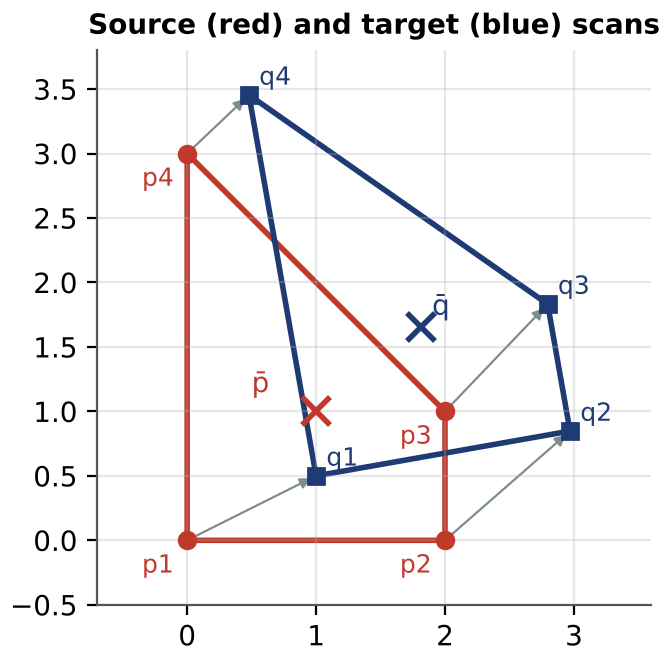
\includegraphics[width=\linewidth]{icp4}
\end{minipage}

\begin{center}\small
\begin{tabular}{rrrrrr}\toprule
$p'_x$&$p'_y$&$q'_x$&$q'_y$&$p'_xq'_x+p'_yq'_y$&$p'_xq'_y-p'_yq'_x$\\\midrule
$-1$&$-1$&$-0.811$&$-1.158$&1.970&0.347\\
$1$&$-1$&$1.158$&$-0.811$&1.970&0.347\\
$1$&$0$&$0.985$&$0.174$&0.985&0.174\\
$-1$&$2$&$-1.332$&$1.796$&4.924&0.868\\\midrule
&&&\textbf{Sum}&\textbf{9.848}&\textbf{1.736}\\\bottomrule
\end{tabular}\end{center}

\begin{worked}{(continued)}
\step{Step 3 --- rotation} $\theta=\operatorname{atan2}(1.736,\ 9.848)=10.00^\circ$
\step{Step 4 --- translation} $\vect t=\bar{\vect q}-\vect R\bar{\vect p}$:\ $\vect R\bar{\vect p}=(0.9848-0.1736,\ 0.1736+0.9848)=(0.811,\ 1.158)$;\ $\vect t=(1.811-0.811,\ 1.658-1.158)=(1.000,\ 0.500)$
\step{Step 5 --- check with SVD} $\vect W=\begin{psmallmatrix}4.287&-1.275\\-3.012&5.562\end{psmallmatrix}$ gives $\vect V\vect U^{\mathsf T}=\begin{psmallmatrix}0.985&-0.174\\0.174&0.985\end{psmallmatrix}$ $=\vect R(10^\circ)$ \checkmark
\result{the second scan is the first rotated 10° and shifted (1.0, 0.5) m --- exactly how the target was made. In real ICP the pairs are only guesses, so steps 1--5 repeat.}
\end{worked}

\section{Better cost functions: point-to-plane and NDT}
\fig[0.95]{p2plane}{Point-to-point pulls toward sample points; point-to-plane only penalizes the gap normal to the surface.}

\begin{keyeq}{Point-to-plane ICP}
\[ E=\sum_i\Big(\big(\vect R\vect p_i+\vect t-\vect q_i\big)\cdot\vect n_i\Big)^2 \]
\begin{symbols}
$\vect n_i$ & unit normal of the target surface at $\vect q_i$ & ---\\
$(\cdot)\cdot\vect n_i$ & dot product: keeps only the part of the gap perpendicular to the surface & m\\
\end{symbols}
\end{keyeq}

\fig[0.55]{ndt}{The Normal Distributions Transform summarizes each grid cell by a mean and covariance.}
\begin{eng}
\textbf{NDT} (Normal Distributions Transform) divides the target into voxels and fits each with a Gaussian (mean $\boldsymbol\mu_k$, covariance $\boldsymbol\Sigma_k$). The source is scored by $\sum_i\exp\!\big(-\tfrac12(\vect x_i-\boldsymbol\mu_k)^{\mathsf T}\boldsymbol\Sigma_k^{-1}(\vect x_i-\boldsymbol\mu_k)\big)$ with $\vect x_i=\vect R\vect p_i+\vect t$, and maximized. No nearest-neighbor search is needed, it is smooth, and it is widely used in automotive localization. \textbf{Generalized ICP} (GICP) blends both ideas by modeling local surface covariances on both clouds.
\end{eng}

\section{Feature-based matching (LOAM and LIO-SAM)}
\fig[0.72]{loam}{Points on sharp corners become edge features; points on smooth surfaces become planar features.}

\begin{kid}
Instead of matching every single dot, look for the \emph{special} ones: sharp corners (like the corner of a box) and flat sides (like a table top). Corners are easy to recognize and flat sides are easy to slide against. Matching only these is much faster.
\end{kid}

\begin{keyeq}{Roughness (curvature) score}
\[ c_i=\frac{1}{|S|\cdot\rho_i}\ \Big|\sum_{j\in S}(\rho_j-\rho_i)\Big| \]
\begin{symbols}
$\rho_i$ & range of point $i$ along one scan line & m\\
$S$ & its neighbors on the same scan line ($|S|$ = how many, e.g.\ 5 each side) & ---\\
$c_i$ & roughness: large $\Rightarrow$ edge feature; small $\Rightarrow$ planar feature & ---\\
\end{symbols}
(Simplified range form; LOAM uses the same expression with 3-D point vectors.)
\end{keyeq}

\begin{worked}{edge or plane?}
\textbf{Given:} two neighbors each side ($|S|=4$).
\step{Flat wall} ranges $10.00,\ 10.01,\ \underline{10.00},\ 9.99,\ 10.00$: sum of differences $=0+0.01-0.01+0=0$ $\Rightarrow c=0$ \quad\textbf{planar}
\step{Corner} ranges $10.0,\ 10.0,\ \underline{8.0},\ 8.0,\ 8.0$: sum $=2+2+0+0=4$ $\Rightarrow c=4/(4\times8)=0.125$ \quad\textbf{edge}
\result{thresholds (e.g.\ $c>0.1$ edge, $c<0.1$ plane in LOAM's default) sort the points.}
\end{worked}

\subsection{Distances to edges and planes (LIO-SAM eqs.\ 10--11)}
\fig[0.92]{edgeplane}{An edge feature is compared with a line through two map points; a planar feature with a plane through three.}

\begin{keyeq}{Point-to-line and point-to-plane distances}
\[ d_e=\frac{\big\|(\vect p-\vect a)\times(\vect p-\vect b)\big\|}{\|\vect a-\vect b\|}\qquad\qquad
d_p=\frac{\big|(\vect p-\vect u)\cdot\big((\vect u-\vect v)\times(\vect u-\vect w)\big)\big|}{\big\|(\vect u-\vect v)\times(\vect u-\vect w)\big\|} \]
\begin{symbols}
$\vect p$ & a feature point of the new scan, transformed into the map frame with the current guess & m\\
$\vect a,\vect b$ & two map points defining the matching edge line ($\vect p^e_{i,u},\vect p^e_{i,v}$ in the paper) & m\\
$\vect u,\vect v,\vect w$ & three map points defining the matching planar patch & m\\
$\times$ & cross product (Module 2): its length is a parallelogram area; area $\div$ base = height = distance & ---\\
$(\vect u-\vect v)\times(\vect u-\vect w)$ & a vector normal to the plane & m$^2$\\
\end{symbols}
\end{keyeq}

\begin{worked}{edge and plane distances}
\step{Edge} $\vect a=(0,0,0)$, $\vect b=(2,0,0)$, $\vect p=(1,0.6,0.8)$.
$\vect p-\vect a=(1,0.6,0.8)$, $\vect p-\vect b=(-1,0.6,0.8)$; cross $=(0.6\cdot0.8-0.8\cdot0.6,\ 0.8\cdot(-1)-1\cdot0.8,\ 1\cdot0.6-0.6\cdot(-1))=(0,-1.6,1.2)$; length $=\sqrt{2.56+1.44}=2.0$; divide by $\|\vect a-\vect b\|=2$: $d_e=1.0$ m.
\step{Plane} $\vect u=(0,0,0)$, $\vect v=(1,0,0)$, $\vect w=(0,1,0)$, $\vect p=(0.3,0.4,0.12)$. Normal $=(\vect u-\vect v)\times(\vect u-\vect w)=(-1,0,0)\times(0,-1,0)=(0,0,1)$; $d_p=|(0.3,0.4,0.12)\cdot(0,0,1)|/1=0.12$ m.
\result{LIO-SAM then finds the pose that minimizes $\sum d_e+\sum d_p$ over all features using the Gauss--Newton method.}
\end{worked}

\begin{eng}
\textbf{Gauss--Newton in one paragraph.} Stack all distances into a residual vector $\vect d(\vect x)$ that depends on the 6-DOF pose $\vect x$. Linearize: $\vect d(\vect x+\delta\vect x)\approx\vect d+\vect J\delta\vect x$, where $\vect J$ is the Jacobian. Setting the derivative of $\|\vect d+\vect J\delta\vect x\|^2$ to zero gives the \emph{normal equations} $\vect J^{\mathsf T}\vect J\,\delta\vect x=-\vect J^{\mathsf T}\vect d$ --- exactly the normal equations of a survey least-squares adjustment. Solve, update $\vect x\leftarrow\vect x+\delta\vect x$, repeat until $\delta\vect x$ is tiny.
\end{eng}

\section{When matching fails: the hallway effect}
\fig[0.98]{hallway}{In a featureless corridor the matching error has a flat valley along the corridor --- any forward shift fits equally well.}

\begin{eng}
Scan matching can only measure motion in directions where geometry changes. In a long uniform corridor, tunnel, or a highway with continuous barriers, the cost is flat along the axis, $\vect J^{\mathsf T}\vect J$ is nearly singular in that direction, and the estimate is free to stretch or shrink. Mathematically, the smallest eigenvalue of $\vect J^{\mathsf T}\vect J$ is near zero; some systems monitor this ``degeneracy'' and down-weight LiDAR along that axis. Surveyors recognize this as a traverse with poor geometry in one direction.
\end{eng}

\begin{tip}
In corridors: add control or targets along the length, walk/drive both directions, include side rooms or cross-ties to create unique geometry, place temporary objects (cones, boxes) if needed, and always check along-track distances against a taped or total-station measurement.
\end{tip}

\begin{tryit}
\textbf{11.1} Source points $(0,0),(1,0)$ match target points $(2,1),(2,2)$. Find $\theta$ and $\vect t$ by the closed form.\\
\textbf{11.2} Distance from $\vect p=(3,4,5)$ to the line through $(0,0,0)$ and $(0,0,10)$?\\
\textbf{11.3} (Simple) Why is it hard to tell how far you have walked in a long, plain hallway with your eyes half-closed?
\end{tryit}

\sources{Besl \& McKay (1992), \emph{IEEE PAMI} 14(2); Arun, Huang \& Blostein (1987), \emph{IEEE PAMI} 9(5); Segal \emph{et al.}\ (2009), Generalized-ICP; Biber \& Stra{\ss}er (2003), NDT; Zhang \& Singh (2017), LOAM, \emph{Autonomous Robots} 41(2); Shan \emph{et al.}\ (2020), eqs.\ (10)--(11).}

\chapter{Factor Graphs and LIO-SAM}

\section{From a filter to a graph}
\begin{kid}
Imagine a row of people connected by rubber bands. Each rubber band says ``you two should be this far apart.'' One person is also tied to a post that says ``you belong here.'' If one band pulls a little wrong, everyone wiggles until the pulling is shared out as fairly as possible. A \textbf{factor graph} is that picture: the people are the car's positions over time, and the rubber bands are measurements.
\end{kid}

\fig[0.95]{factorgraph}{A factor graph: circles are unknown states (poses); small squares are measurements (factors) that tie them together.}

\begin{eng}
A filter (EKF) processes data once and forgets the past. A \textbf{smoother} keeps the whole trajectory as unknowns and re-solves when new information arrives --- so a loop closure at minute 20 can correct the pose at minute 3. The data structure is a \textbf{factor graph}: \emph{variable nodes} $\vect x_i$ (poses, velocities, IMU biases) and \emph{factor nodes}, each encoding one measurement as a probability that depends on a few variables. Assuming Gaussian noise, finding the most probable trajectory (maximum a posteriori, MAP) is exactly a non-linear weighted least-squares problem --- the same mathematics as a survey network adjustment.
\end{eng}

\begin{keyeq}{MAP estimation becomes least squares}
\[ \vect X^*=\arg\max_{\vect X}\prod_k\phi_k(\vect X_k)=\arg\min_{\vect X}\sum_k\big\|\vect h_k(\vect X_k)-\vect z_k\big\|^2_{\boldsymbol\Sigma_k} \]
\begin{symbols}
$\vect X$ & all unknowns together (every pose, velocity, bias) & ---\\
$\vect X^*$ & the best (most probable) solution & ---\\
$\phi_k$ & factor $k$: a Gaussian probability $\propto\exp(-\tfrac12\|\cdot\|^2_{\Sigma})$ & ---\\
$\vect X_k$ & only the few variables factor $k$ touches & ---\\
$\vect h_k$ & measurement model: what factor $k$ \emph{should} measure given $\vect X_k$ & ---\\
$\vect z_k$ & what it actually measured & ---\\
$\|\vect e\|^2_{\boldsymbol\Sigma}=\vect e^{\mathsf T}\boldsymbol\Sigma^{-1}\vect e$ & squared Mahalanobis distance: residuals divided by their uncertainty (weights $=\boldsymbol\Sigma^{-1}$) & ---\\
\end{symbols}
Taking $-\log$ of a product of Gaussians turns ``maximize the product'' into ``minimize the sum of squares.''
\end{keyeq}

\section{A factor graph you can solve by hand}
\fig[0.95]{fg1d}{Four positions along a straight road, three odometry factors, one GPS factor and a prior.}

\begin{worked}{1-D pose graph with a GPS misclosure}
\textbf{Given:} $x_0=0$ (fixed prior). LiDAR odometry: $x_1-x_0=1.0$, $x_2-x_1=1.1$, $x_3-x_2=0.9$ m. GPS: $x_3=3.2$ m. All four measurements have the same $\sigma=0.10$ m (equal weights).
\step{Step 1 --- write the residual equations $\vect A\vect x=\vect b$}
\[ \begin{pmatrix}1&0&0\\-1&1&0\\0&-1&1\\0&0&1\end{pmatrix}\begin{pmatrix}x_1\\x_2\\x_3\end{pmatrix}=\begin{pmatrix}1.0\\1.1\\0.9\\3.2\end{pmatrix} \]
\step{Step 2 --- normal equations $\vect A^{\mathsf T}\vect A\,\vect x=\vect A^{\mathsf T}\vect b$}
\[ \begin{pmatrix}2&-1&0\\-1&2&-1\\0&-1&2\end{pmatrix}\vect x=\begin{pmatrix}1.0-1.1\\1.1-0.9\\0.9+3.2\end{pmatrix}=\begin{pmatrix}-0.1\\0.2\\4.1\end{pmatrix} \]
\step{Step 3 --- solve} From row 1: $x_2=2x_1+0.1$. Row 2: $-x_1+2(2x_1+0.1)-x_3=0.2\Rightarrow x_3=3x_1$. Row 3: $-(2x_1+0.1)+6x_1=4.1\Rightarrow x_1=1.05$. Then $x_2=2.20$, $x_3=3.15$.
\step{Step 4 --- residuals} odometry: $1.05-1.0=+0.05$, $1.15-1.1=+0.05$, $0.95-0.9=+0.05$; GPS: $3.15-3.2=-0.05$
\result{$x_1=1.05$, $x_2=2.20$, $x_3=3.15$ m. The 0.20 m misclosure is shared equally by the four equally weighted measurements --- the compass/least-squares adjustment of a traverse, done by a factor graph.}
\end{worked}

\begin{eng}
Notice $\vect A^{\mathsf T}\vect A$ is \emph{sparse} (mostly zeros): each pose only links to its neighbors. Real graphs have tens of thousands of nodes (LIO-SAM's Amsterdam run: 23\,304 nodes, 49\,617 factors) but stay sparse, so they solve quickly. \textbf{iSAM2} (incremental smoothing and mapping with the Bayes tree) goes further: when a new node arrives it re-solves only the part of the graph that changed, which is how LIO-SAM runs in real time. GTSAM is the open-source library implementing it.
\end{eng}

\section{LIO-SAM, piece by piece}
LIO-SAM (Shan, Englot, Meyers, Wang, Ratti \& Rus, IROS 2020) is a \emph{tightly-coupled} lidar--inertial odometry and mapping system built on a factor graph. ``Tightly coupled'' means the IMU and LiDAR are optimized \emph{together} (the IMU biases are estimated from the LiDAR results), rather than the IMU merely supplying a guess.

\begin{keyeq}{The LIO-SAM state (paper eq.\ 1)}
\[ \vect x=\big[\vect R^{\mathsf T},\ \vect p^{\mathsf T},\ \vect v^{\mathsf T},\ \vect b^{\mathsf T}\big]^{\mathsf T},\qquad \vect T=[\vect R\mid\vect p]\in SE(3) \]
\begin{symbols}
$\vect R\in SO(3)$ & attitude (body to world) & ---\\
$\vect p\in\mathbb R^3$ & position & m\\
$\vect v$ & velocity & m/s\\
$\vect b$ & IMU biases (gyro and accelerometer) & rad/s, m/s$^2$\\
$\vect T$ & pose as a rigid transform (Module 6) & ---\\
\end{symbols}
\end{keyeq}

\subsection{The four factors}
\begin{center}\small
\renewcommand{\arraystretch}{1.25}
\begin{tabularx}{\linewidth}{>{\bfseries}p{2.6cm}XX}\toprule
Factor & What it measures & Surveying analog\\\midrule
\color{orange}IMU preintegration & relative motion $\Delta\vect v_{ij},\Delta\vect p_{ij},\Delta\vect R_{ij}$ between consecutive states (Module 7) & a measured distance and angle between traverse stations\\
\color{teal}LiDAR odometry & relative transform $\Delta\vect T_{i,i+1}=\vect T_i^{-1}\vect T_{i+1}$ from scan-to-map matching (Module 11) & a second, independent set of traverse observations\\
\color{gold}GPS & absolute position of a state (converted to local Cartesian) & tying a station to a control point\\
\color{purple}Loop closure & relative transform between a new state and an old nearby one & closing the traverse on itself\\\bottomrule
\end{tabularx}\end{center}

\subsection{Keyframes and the sliding window}
\fig[0.95]{keyframes}{Only keyframes enter the graph; a new keyframe is matched to a local map of the last $n$ sub-keyframes.}

\begin{eng}
Adding every LiDAR frame (10 per second) would make the graph enormous. LIO-SAM adds a new state $\vect x_{i+1}$ (a \textbf{keyframe}) only when the pose changes by more than \textbf{1 m} or \textbf{10°}; frames in between are discarded. To create a LiDAR odometry factor:
\begin{enumerate}
\item extract edge and planar features from the new de-skewed scan (roughness, Module 11);
\item transform the last $n=25$ keyframes (``sub-keyframes'') into the world frame and merge them into a local voxel map $\vect M_i=\{\vect M^e_i,\vect M^p_i\}$, down-sampled at 0.2 m (edges) and 0.4 m (planes);
\item using the IMU-predicted pose $\tilde{\vect T}_{i+1}$ as the starting guess, find edge/plane correspondences and minimize $\sum d_e+\sum d_p$ by Gauss--Newton;
\item the relative transform to the previous state becomes the factor.
\end{enumerate}
Matching to a small local map, rather than a global one as in LOAM, is the main reason LIO-SAM is fast.
\end{eng}

\subsection{GPS and loop-closure factors}
\begin{eng}
\textbf{GPS factor.} GPS is converted to a local Cartesian frame; if not hardware-synchronized it is linearly interpolated to the keyframe time. Because lidar--inertial drift grows slowly, a GPS factor is added only when the estimated position covariance is \emph{larger} than the GPS covariance --- a sensible ``only use control when you need it'' rule.

\textbf{Loop-closure factor.} When a new state is added, LIO-SAM searches for earlier states within \textbf{15 m}. For a candidate $\vect x_3$, the new keyframe is matched to the $2m+1$ keyframes around it ($m=12$), giving $\Delta\vect T_{3,i+1}$ as a factor. The authors note loop closures are especially valuable for correcting \emph{altitude}, where GPS was poor (errors approaching 100 m without loops in their tests).
\end{eng}

\subsection{What it achieved}
\begin{center}\small
\begin{tabular}{lrrrrr}\toprule
\multicolumn{6}{c}{\textbf{End-to-end translation error (m; LIO-SAM in ft in parentheses) --- LIO-SAM paper, Table II}}\\\midrule
Dataset & LOAM & LIOM & LIO-odom & LIO-GPS & LIO-SAM\\\midrule
Campus (1.4 km / 0.9 mi) & 192.43 & fail & 9.44 & 6.87 & \textbf{0.12} (0.39 ft)\\
Park (2.9 km / 1.8 mi) & 121.74 & 34.60 & 36.36 & 2.93 & \textbf{0.04} (0.13 ft)\\
Amsterdam (19 km / 11.8 mi) & fail & fail & fail & 1.21 & \textbf{0.17} (0.56 ft)\\\bottomrule
\end{tabular}\end{center}
\textit{LIO-odom} uses only IMU + LiDAR factors; \textit{LIO-GPS} adds GPS; full \textit{LIO-SAM} adds loop closures. Each extra factor type removes another layer of drift. LIO-SAM processed scans in 42--101 ms and ran up to 13$\times$ faster than real time.

\begin{improve}
These are research-grade results judged against the start/end point or GPS, on a robot, not survey-grade checkpoint accuracy. A 4--17 cm loop misclosure over kilometers is excellent odometry, but a deliverable still needs calibration, control and \emph{independent checkpoints} (Module 13) before any accuracy can be stated. Also, the paper's eq.\ (12) writes $\Delta\vect T=\vect T_i^{\mathsf T}\vect T_{i+1}$; the correct general form is $\vect T_i^{-1}\vect T_{i+1}$.
\end{improve}

\begin{tip}
You do not need to write an optimizer, but you should be able to answer: Which factors were active in this dataset? Where were the loop closures? Where was GNSS used? Where did the corridor degrade LiDAR odometry? Good processing software lets you view the trajectory colored by its estimated standard deviation --- inspect it before trusting any part of the cloud.
\end{tip}

\section{Building the trajectory: poses, scans, IMU, GNSS and images}
\begin{kid}
Think of a trip recorded as a flip-book. Each page is a \textbf{pose}: where the car was and which way it was pointing at one instant. The IMU writes a new page hundreds of times a second, so the flip-book is smooth --- but it slowly drifts. The LiDAR compares each new scan with the last ones and corrects the drift, like recognizing the same buildings. GNSS now and then says ``this page is exactly here on Earth.'' The camera takes pictures along the way, and each picture is glued to the page for the moment it was taken. Flip through all the pages and you have the \textbf{trajectory}: the path, with direction, at every instant.
\end{kid}

\subsection*{The words}
\begin{center}\small
\renewcommand{\arraystretch}{1.2}
\begin{tabularx}{\linewidth}{>{\bfseries}p{3.0cm}X}\toprule
Pose & position ($X,Y,Z$) \emph{and} orientation (roll, pitch, yaw) at one instant (Module 6)\\
Trajectory & the continuous sequence of poses over time --- the ``path with direction'' (often delivered as a time-stamped file, e.g.\ an SBET or a pose table)\\
Keyframe pose & a pose that is a node in the factor graph (LIO-SAM: every 1 m or 10°)\\
Interpolated pose & a pose computed \emph{between} keyframes for any time you need: each laser pulse, each image\\
Image pose & the camera's pose at exposure time (photogrammetrists call it exterior orientation): trajectory pose + camera lever arm and boresight\\\bottomrule
\end{tabularx}\end{center}

\fig[1.0]{traj_timeline}{One second of data. The IMU ticks 200 times, the LiDAR completes 10 sweeps, GNSS gives 5 fixes and the camera takes 2 images. The trajectory (top row) is the common thread that gives every one of them a pose.}

\subsection*{What each sensor contributes}
\begin{center}\small
\renewcommand{\arraystretch}{1.25}
\begin{tabularx}{\linewidth}{>{\bfseries}p{2.0cm}>{\raggedright\arraybackslash}p{1.4cm}XX}\toprule
Sensor & Rate & Contributes to the trajectory & Cannot do\\\midrule
\color{teal}IMU & 100--1000 Hz & smooth, high-rate motion between everything else; roll and pitch from gravity; de-skews every LiDAR sweep; bridges gaps (preintegration factors) & stay accurate on its own for more than seconds; give absolute position\\
\color{orange}LiDAR scans & 10--20 Hz & relative motion from scan matching (odometry factors); heading and drift control wherever there is geometry; loop closures when places are revisited; the map itself & work in featureless places (corridors, open fields); give absolute coordinates\\
\color{gold}GNSS & 1--20 Hz & absolute position in the datum (GNSS factors); stops long-term drift; RTK makes it centimeter-level; dual antenna adds heading & work in tunnels, under canopy, indoors; supply attitude at high rate\\
\color{purple}Camera images & 1--10 Hz & in LIO-SAM: nothing --- images \emph{receive} poses. (Visual--inertial systems also use image features as extra odometry.) & ---\\
\textbf{Control} & a few points & ties the whole trajectory to surveyed coordinates; checkpoints prove it & ---\\\bottomrule
\end{tabularx}\end{center}

\fig[0.98]{traj_map}{The path as built: blue trajectory with pose axes, orange LiDAR scan coverage used for matching, gold GNSS fixes (absent in the tunnel), and purple camera images, each placed with its own interpolated pose.}

\fig[0.9]{traj_share}{Conceptually, the factor graph leans on whichever sensors have information at each moment: LiDAR and IMU carry the tunnel; GNSS and IMU carry the featureless field.}

\begin{worked}{giving a camera image its pose}
\textbf{Given:} trajectory poses at $t_1=10.00$ s: $E=100.00$, $N=200.00$ m, heading $30.0^\circ$; at $t_2=10.10$ s: $E=101.50$, $N=200.10$ m, heading $31.0^\circ$. A photo is exposed at $t=10.04$ s.
\step{Step 1 --- fraction of the way} $f=(10.04-10.00)/(10.10-10.00)=0.4$
\step{Step 2 --- position} $E=100.00+0.4(1.50)=100.60$ m;\ $N=200.00+0.4(0.10)=200.04$ m
\step{Step 3 --- heading} $30.0+0.4(1.0)=30.4^\circ$ (real software interpolates the full rotation, e.g.\ quaternion ``slerp'')
\step{Step 4 --- camera offset} apply the camera's lever arm and boresight (Module 9) to move from the IMU to the lens
\result{the image pose is $(100.60,\ 200.04)$, heading $30.4^\circ$. The same interpolation gives every one of the millions of laser pulses its pose.}
\end{worked}

\begin{worked}{why the camera needs calibration and timing too}
\step{Boresight error $0.1^\circ$, point 20 m away} $20\times0.001745=0.035$ m --- colors land 3.5 cm off their points
\step{Timing error 5 ms at 10 m/s} $10\times0.005=0.05$ m --- colors smear 5 cm along the road
\result{colorized point clouds and photo-measured features inherit every trajectory error \emph{plus} the camera's own calibration and timing errors. Calibrate and synchronize the camera like the LiDAR (Modules 8--9).}
\end{worked}

\begin{tip}
\textbf{Deliver and archive the trajectory.} Keep the final trajectory (time, position, attitude and their standard deviations), the image exterior orientations, the calibration file and the processing log with the project. When a client later asks ``where did this point come from?'', the trajectory is the answer --- and it is the first thing a reviewer will inspect for drift, gaps and GNSS outages.
\end{tip}

\begin{tryit}
\textbf{12.1} Repeat the 1-D example with GPS saying $x_3=3.0$. What happens and why?\\
\textbf{12.2} Repeat with GPS $x_3=3.2$ but GPS $\sigma=0.05$ m (weight 4$\times$ the others). Solve the weighted normal equations.\\
\textbf{12.3} (Simple) In the rubber-band picture, what happens if one band is much stiffer than the rest?
\end{tryit}

\sources{Shan \emph{et al.}\ (2020), LIO-SAM (Tables I--IV, keyframe and loop-closure parameters); Kaess, M.\ \emph{et al.}\ (2012), iSAM2, \emph{Int.\ J.\ Robotics Research} 31(2); Dellaert \& Kaess (2017), Factor graphs for robot perception.}

\chapter{Control, Error Budgets and Accuracy Standards}

\section{Relative versus absolute}
\begin{kid}
You can draw a perfect map of your bedroom --- every toy in the right place compared to every other toy --- but if you don't know where your house is on the street, nobody else can use it to find your room. SLAM makes the bedroom map. \textbf{Control points} --- spots measured very carefully by surveyors --- pin that map onto the real world. \textbf{Checkpoints} are extra careful spots that we keep secret from the computer, then use to test whether the map is truly right.
\end{kid}

\fig[0.82]{control}{Along a corridor, alternate points used to constrain the solution (control) with points held back purely to test it (checkpoints).}

\begin{eng}
SLAM and lidar--inertial odometry are \emph{relative}: internally consistent but floating in their own frame and slowly drifting. GNSS and surveyed \textbf{control} fix the datum (horizontal and vertical) and constrain drift. Accuracy claims, however, must come from \textbf{independent checkpoints} --- surveyed points \emph{not} used in any adjustment. Using the same points for both makes the residuals look artificially small, exactly as reporting the residuals of a constrained adjustment at its own fixed stations would. Document which points were used for what.
\end{eng}

\begin{tip}
\begin{itemize}
\item Use targets the scanner can see and the software can measure: painted chevrons or checkerboards on pavement for vertical and horizontal checks; high-intensity paint shows clearly in intensity.
\item Survey control and checkpoints with a method at least \textbf{two times} more accurate than the product you are testing (ASPRS Edition 2), and include their own uncertainty in the final accuracy (below).
\item Distribute checkpoints along the whole project and across the cross-section --- not only at the ends near GNSS-friendly areas.
\item Confirm the vertical datum and geoid model match project requirements before comparing anything.
\end{itemize}
\end{tip}

\section{Computing accuracy from checkpoints}
\fig[0.78]{residuals}{Vertical residuals (LiDAR surface minus surveyed elevation) at ten checkpoints.}

\begin{keyeq}{Accuracy statistics}
\[ \text{RMSE}_z=\sqrt{\frac1n\sum_{i=1}^n\Delta z_i^2},\qquad
\text{RMSE}_H=\sqrt{\text{RMSE}_x^2+\text{RMSE}_y^2} \]
\[ \text{RMSE}_{\text{final}}=\sqrt{\text{RMSE}_{\text{data}}^2+\text{RMSE}_{\text{survey}}^2} \]
\begin{symbols}
$\Delta z_i$ & LiDAR elevation minus checkpoint elevation at point $i$ & m\\
$n$ & number of checkpoints (ASPRS Ed.\ 2: at least 30 for a formal product test) & ---\\
$\text{RMSE}_x$,\newline$\text{RMSE}_y$ & RMSE of easting and northing differences & m\\
$\text{RMSE}_H$ & horizontal (radial) RMSE & m\\
{\footnotesize$\text{RMSE}_{\text{survey}}$} & uncertainty of the checkpoint survey itself & m\\
{\footnotesize$\text{RMSE}_{\text{final}}$} & accuracy to report, including checkpoint error (Ed.\ 2 requirement) & m\\
\end{symbols}
\end{keyeq}

\begin{worked}{vertical accuracy from ten checkpoints}
\textbf{Given (cm):} $\Delta z=+2.1,\ -3.4,\ +1.2,\ +4.5,\ -0.8,\ +2.7,\ -1.9,\ +3.1,\ +0.4,\ -2.6$. Checkpoints surveyed with RMSE 1.0 cm.
\step{Step 1 --- mean (bias)} sum $=5.3$; $\bar e=5.3/10=+0.53$ cm (no meaningful bias)
\step{Step 2 --- squares} $4.41,\ 11.56,\ 1.44,\ 20.25,\ 0.64,\ 7.29,\ 3.61,\ 9.61,\ 0.16,\ 6.76$; sum $=65.73$
\step{Step 3 --- RMSE} $\sqrt{65.73/10}=\sqrt{6.573}=2.56$ cm
\step{Step 4 --- std.\ dev.} $s=2.64$ cm (computed as in Module 2)
\step{Step 5 --- include checkpoint error} $\sqrt{2.56^2+1.0^2}=\sqrt{7.57}=2.75$ cm
\result{report non-vegetated vertical accuracy $\text{RMSE}_z=2.8$ cm (Edition 2 style). Ten points are fine for a quick field check, but a formal ASPRS test needs at least 30.}
\end{worked}

\begin{worked}{horizontal accuracy}
\textbf{Given:} $\text{RMSE}_x=2.25$ cm and $\text{RMSE}_y=2.16$ cm from five well-defined points.
\step{Combine} $\text{RMSE}_H=\sqrt{2.25^2+2.16^2}=\sqrt{5.06+4.67}=3.12$ cm
\result{3.1 cm horizontal (radial) RMSE.}
\end{worked}

\section{The accuracy standards you will report against}
\begin{eng}
\textbf{ASPRS Positional Accuracy Standards for Digital Geospatial Data, Edition 2} (2023; Version 2, 2024) is the reference most US contracts cite. Key changes from Edition 1 that affect mobile LiDAR:
\begin{itemize}
\item accuracy is stated as \textbf{RMSE only} --- the old ``95\% confidence'' figures ($1.96\times\text{RMSE}_z$, $1.7308\times\text{RMSE}_r$) are no longer reported;
\item minimum \textbf{30 checkpoints} for product assessment (up to 120 for large projects);
\item ground control and checkpoints must be at least \textbf{2$\times$} more accurate than the product;
\item checkpoint survey error must be \textbf{included} in the reported accuracy;
\item vegetated vertical accuracy (VVA) is reported ``as found''; acceptance rests on non-vegetated accuracy (NVA).
\end{itemize}
\textbf{Florida.} Surveys and maps prepared by Florida Professional Surveyors and Mappers must meet the Standards of Practice in \textbf{Chapter 5J-17, Florida Administrative Code}. In practice that means the responsible surveyor states the methods used, the horizontal and vertical datums, and the accuracy achieved and how it was verified, and signs for data captured by remote sensing just as for conventional measurements. FDOT publishes separate guidance for terrestrial mobile LiDAR on its projects. Rules are amended periodically --- always work from the current rule text and the client's specification, not from a course book.
\end{eng}

\begin{improve}
The seminar's error-budget slide used ``5 cm horizontal at 95\% confidence.'' Under ASPRS Edition 2 the same requirement would be written as an RMSE. If a specification still quotes a 95\% value, convert carefully: for vertical, $\text{RMSE}_z=\text{Acc}_{95}/1.96$; for horizontal, $\text{RMSE}_H=\text{Acc}_{95}/1.7308$ (valid when $\text{RMSE}_x\approx\text{RMSE}_y$), so 5 cm at 95\% horizontal $\approx$ 2.9 cm $\text{RMSE}_H$ --- a much tighter target than ``5 cm'' sounds, and one the budget below (4.2 cm, 1$\sigma$ per component) would \emph{not} meet. Units and confidence levels must be settled before the budget is written.
\end{improve}

\section{ASPRS lidar data standards in detail}
Two ASPRS documents govern almost every LiDAR deliverable in the United States: the \textbf{Positional Accuracy Standards for Digital Geospatial Data} (Edition 2, Version 2, 2024), which say how accurate the data are and how that is proven, and the \textbf{LAS Specification} (version 1.4), which says how the points are stored and labeled. Client specifications --- FDOT, USGS and others --- build on both.

\begin{kid}
One rulebook says \emph{how close to the truth} the dots must be and how to check them with secret checkpoints. The other rulebook says \emph{how to write the dots down} in a file, including a label on every dot: ground, building, tree, water, wire, noise\ldots{} so any software can read it.
\end{kid}

\subsection{Accuracy classes (Edition 2)}
\begin{eng}
Edition 2 defines accuracy classes directly by RMSE, in any size the project needs: a ``5 cm vertical accuracy class'' means $\text{RMSE}_V\le5$ cm; a ``3 cm horizontal accuracy class'' means $\text{RMSE}_H\le3$ cm.
\begin{itemize}
\item \textbf{NVA} (non-vegetated vertical accuracy), tested on open hard or bare surfaces, decides \textbf{acceptance}.
\item \textbf{VVA} (vegetated vertical accuracy) is tested and \textbf{reported as found}, with no pass/fail threshold unless the client and producer agree otherwise.
\item \textbf{Checkpoints:} at least 30 for NVA (up to 120 for large projects) and at least 30 for VVA, well distributed; independent of any control used for calibration or boresighting; at least \textbf{2$\times$ more accurate} than the product.
\item \textbf{Control} for calibration should likewise be twice as accurate as the product (e.g.\ $\text{RMSE}_V(\text{control})\le\tfrac12\,\text{RMSE}_V(\text{product})$).
\item \textbf{Product accuracy includes checkpoint error:} $\text{RMSE}_{\text{product}}=\sqrt{\text{RMSE}_{\text{fit}}^2+\text{RMSE}_{\text{survey}}^2}$ (Module 13 worked example).
\item \textbf{Horizontal accuracy of lidar} is usually not tested point by point (points do not land on well-defined corners) but estimated from GNSS and IMU error and range/altitude, or tested on well-defined features when density allows. For mobile LiDAR, painted chevrons and building corners make horizontal testing practical.
\end{itemize}
\end{eng}

\subsection{Data internal precision (relative accuracy)}
\begin{center}\small
\renewcommand{\arraystretch}{1.2}
\begin{tabular}{lcccc}\toprule
\textbf{Vertical class $X$} & \textbf{NVA $\text{RMSE}_V$} & \textbf{Within-swath} & \textbf{Swath-to-swath} & \textbf{Swath-to-swath}\\
 & & \textbf{smooth-surface max diff.} & \textbf{RMSD$_z$} & \textbf{max diff.}\\\midrule
General rule & $\le X$ & $\le0.6X$ & $\le0.8X$ & $\le1.6X$\\
5 cm (0.16 ft) class & $\le5$ cm / 0.16 ft & $\le3$ cm / 0.10 ft & $\le4$ cm / 0.13 ft & $\le8$ cm / 0.26 ft\\
10 cm (0.33 ft) class & $\le10$ cm / 0.33 ft & $\le6$ cm / 0.20 ft & $\le8$ cm / 0.26 ft & $\le16$ cm / 0.52 ft\\\bottomrule
\end{tabular}\end{center}
{\footnotesize Source: ASPRS Positional Accuracy Standards, Edition 2, Version 2 (2024), Table 7.2, which gives the lidar data internal precision limits as $0.60X$, $0.80X$ and $1.60X$ of the vertical accuracy class $X$ (verified October 2026).}

These are \emph{precision} checks, not accuracy: \textbf{within-swath} tests how smooth a flat surface (a parking lot) is in a single pass --- range noise; \textbf{swath-to-swath} tests how well overlapping passes agree --- trajectory and calibration (the cloud-to-cloud check of Module 18). A project can pass NVA at the checkpoints and still fail swath-to-swath agreement between them.

\subsection{Reporting statements}
\begin{eng}
Edition 2 prescribes the wording:
\begin{itemize}
\item \textbf{Tested (30 or more checkpoints):} ``This data set was tested to meet ASPRS Positional Accuracy Standards for Digital Geospatial Data, Edition 2, Version 2 (2024) for a \_\_ (cm) RMSE$_V$ Vertical Accuracy Class. NVA accuracy was found to be RMSE$_V$ = \_\_ cm.'' VVA is reported the same way, as found.
\item \textbf{Fewer than 30 checkpoints:} the statement must say so: ``\ldots this test was performed using ONLY \_\_ checkpoints.''
\item \textbf{Produced to meet (no independent test):} ``This data set was produced to meet ASPRS Positional Accuracy Standards\ldots'' --- a declaration by the producer only. Calibration control may not be reused as checkpoints.
\end{itemize}
\end{eng}

\subsection{The LAS 1.4 file standard}
\begin{eng}
\begin{itemize}
\item \textbf{Format:} LAS 1.4 (compressed LAZ is the common delivery form). Point data record formats 6--10 are the modern ones: 6 = base (x, y, z, intensity, return number, classification, scan angle, GPS time\ldots); 7 adds RGB; 8 adds RGB + NIR; 9 and 10 add waveform.
\item \textbf{Time:} \emph{Adjusted Standard GPS Time} (GPS seconds minus $10^9$), so every point can be traced back to the trajectory.
\item \textbf{Coordinate system:} stored in the header as OGC WKT, including the vertical datum; it must match the report.
\item \textbf{Classification codes} (ASPRS standard): 
\end{itemize}
\begin{center}\small
\footnotesize\begin{tabular}{rl@{\hspace{1em}}rl@{\hspace{1em}}rl}\toprule
1&Unclassified & 7&Low point (noise) & 14&Wire --- conductor\\
2&Ground & 9&Water & 15&Transmission tower\\
3&Low vegetation & 10&Rail & 17&Bridge deck\\
4&Medium vegetation & 11&Road surface & 18&High noise\\
5&High vegetation & 13&Wire --- guard (shield) & 19&Overhead structure\\
6&Building & 20&Ignored ground & 21/22&Snow / temporal excl.\\\bottomrule
\end{tabular}\end{center}
\end{eng}

\subsection{USGS quality levels (for context)}
Clients often cite the \textbf{USGS Lidar Base Specification} for airborne elevation data: QL0 ($\ge$8 points/m$^2$, NVA RMSE$_z\le5$ cm), QL1 ($\ge$8 pts/m$^2$, $\le10$ cm), QL2 ($\ge$2 pts/m$^2$, $\le10$ cm). Mobile LiDAR easily exceeds these densities; its specifications are usually written project by project, which is why a signed client accuracy agreement (Appendix E) matters.

\section{Error budgets}
Before a job, list every error source you expect and combine them into a total --- an \emph{error budget} --- to confirm the agreed accuracy class is achievable. All of the course's error budgets, from a single traverse-style example to the OS0, GX5/GQ7, RIEGL and capstone systems, are kept together in \textbf{Module 14} (Section~\ref{sec:budgets}).

\begin{tryit}
\textbf{13.1} Checkpoint residuals (cm): $3,-1,2,-2,4$. Compute mean, RMSE, and RMSE including 1.5 cm checkpoint error.\\
\textbf{13.2} A budget has terms 1, 2, 2 and 4 cm. What is the total? Which term would you attack first?\\
\textbf{13.3} (Simple) Why must we keep checkpoints a secret from the computer?
\end{tryit}

\sources{ASPRS (2024), \emph{Positional Accuracy Standards for Digital Geospatial Data}, Edition 2, Version 2 (checkpoints, NVA/VVA, Table 7.2, reporting statements); ASPRS \emph{LAS Specification} 1.4; USGS \emph{Lidar Base Specification} (quality levels); LIDAR Magazine overviews of Edition 2.}

\chapter{Error Propagation and Error Budgets}

Module 2 introduced the root-sum-square rule for independent errors. This module shows \emph{where} each term comes from, how to handle errors that are \emph{not} independent, how errors spread through the full georeferencing equation, and how to check the math with a simulation. It then collects \textbf{every error budget in the course} in one place (Sections~\ref{sec:budgets} and following): a general job budget and the budgets for the OS0 backpack, the GX5/GQ7 IMUs, the RIEGL airborne system and the capstone corridor.

\section{Three kinds of error}
\begin{kid}
Imagine throwing darts. If your darts land all over the board, that is \textbf{random error} --- your hand shakes a little differently every time. If all your darts land in a tight group, but always 5 cm to the left of the bullseye, that is \textbf{systematic error} --- maybe the board is crooked. If one dart hits the wall, that is a \textbf{blunder}. You fix each one in a different way: practice to shrink random error, straighten the board to remove systematic error, and throw out the dart that hit the wall.
\end{kid}

\begin{center}\small
\renewcommand{\arraystretch}{1.25}
\begin{tabularx}{\linewidth}{>{\bfseries}lXXX}\toprule
Type & What it looks like & LiDAR examples & How to handle it\\\midrule
Random & scatter around the true value; different every time & range noise, angle-encoder jitter, IMU white noise & average it, weight it, propagate it with $\sigma$\\
Systematic & same offset (or same pattern) every time & range bias, boresight residual, wrong lever arm, wrong geoid, clock offset & calibrate it, model it, or cancel it by differencing; averaging does \emph{not} help\\
Blunder & a single large, impossible value & wrong antenna height, mixed pixel, multipath jump, wrong datum & detect it (residual tests, checkpoints), then remove it\\\bottomrule
\end{tabularx}\end{center}

\begin{eng}
\textbf{Precision} describes random error (spread). \textbf{Accuracy} describes total closeness to the truth (spread \emph{and} bias). A sensor datasheet usually quotes both separately --- the Ouster OS0 in Module 15 lists ``range precision'' (1$\sigma$ of 100 repeated shots) and ``range accuracy'' (error of their mean). Propagation formulas work on standard deviations and covariances; a bias must be carried separately or converted to an equivalent standard deviation with a stated assumption.
\end{eng}

\section{The law of propagation of variances (one output)}
\fig[0.68]{ep_linear}{Near the operating point the model is almost a straight line. Its slope converts input spread into output spread.}

\begin{keyeq}{Propagation for one output and independent inputs}
\[ y=f(x_1,x_2,\ldots,x_n)\qquad\Longrightarrow\qquad \sigma_y^2=\sum_{i=1}^{n}\left(\frac{\partial f}{\partial x_i}\right)^{2}\sigma_{x_i}^2 \]
\begin{symbols}
$y$ & the computed result (a coordinate, a height, a distance\ldots) & varies\\
$f$ & the formula that computes it & ---\\
$x_i$ & the measured inputs (range, angles, pose\ldots) & varies\\
$\partial f/\partial x_i$ & partial derivative: how much $y$ changes when only $x_i$ changes by one unit (the ``sensitivity'' or ``slope'') & units of $y$ per unit of $x_i$\\
$\sigma_{x_i}$ & standard deviation of input $i$ & units of $x_i$\\
$\sigma_y$ & standard deviation of the result & units of $y$\\
\end{symbols}
\end{keyeq}

\begin{eng}
\textbf{Where it comes from.} Expand $f$ in a first-order Taylor series about the measured values: $y\approx f(\bar{\vect x})+\sum_i\frac{\partial f}{\partial x_i}\delta x_i$. The error in $y$ is a weighted sum of the input errors, $\delta y=\sum a_i\delta x_i$ with $a_i=\partial f/\partial x_i$. For a weighted sum of independent zero-mean errors, $E[\delta y^2]=\sum a_i^2E[\delta x_i^2]$ because all cross terms $E[\delta x_i\delta x_j]$ vanish. That is the formula. It is exact for linear models and an excellent approximation when the errors are small compared with the curvature of $f$ --- true for almost everything in surveying.

\textbf{Two special cases you already know.} If $y=x_1+x_2$, both slopes are 1 and $\sigma_y=\sqrt{\sigma_1^2+\sigma_2^2}$ (root-sum-square). If $y=kx$, then $\sigma_y=|k|\sigma_x$ --- e.g.\ $\rho=c\,\Delta t/2$ gives $\sigma_\rho=(c/2)\sigma_t$ (Module 3).
\end{eng}

\begin{worked}{height of a ground point seen by a scanner}
\textbf{Given:} scanner 2.00 m above a flat road; a road point 20.00 m away horizontally. Range precision $\sigma_\rho=0.35$ cm (dark asphalt at 20 m); vertical-angle accuracy $\sigma_V=0.01^\circ$. Model: $z=\rho\sin V$.
\step{Step 1 --- geometry} $\rho=\sqrt{20^2+2^2}=20.100$ m;\ $V=-\arctan(2/20)=-5.711^\circ$; $\sin V=-0.09950$, $\cos V=0.99504$
\step{Step 2 --- sensitivities} $\partial z/\partial\rho=\sin V=-0.0995$;\quad $\partial z/\partial V=\rho\cos V=20.000$ m/rad
\step{Step 3 --- convert angle to radians} $\sigma_V=0.01\times\pi/180=1.745\times10^{-4}$ rad
\step{Step 4 --- each contribution} range: $0.0995\times0.35=0.035$ cm;\quad angle: $20.000\times1.745\times10^{-4}=0.00349$ m $=0.349$ cm
\step{Step 5 --- combine} $\sigma_z=\sqrt{0.035^2+0.349^2}=0.351$ cm
\result{3.5 mm. Notice that on a grazing road surface the \emph{angle} error, not the range error, controls the height --- range noise points almost horizontally and barely moves $z$. On a wall straight ahead, the opposite is true.}
\end{worked}

\section{When errors are correlated}
\begin{keyeq}{Propagation with covariance}
\[ \sigma_y^2=\sum_i a_i^2\sigma_i^2+2\sum_{i<j}a_ia_j\,\sigma_{ij},\qquad \sigma_{ij}=r_{ij}\,\sigma_i\sigma_j \]
\begin{symbols}
$a_i$ & sensitivity $\partial f/\partial x_i$ & ---\\
$\sigma_{ij}$ & covariance of inputs $i$ and $j$ (how much they move together) & product of units\\
$r_{ij}$ & correlation coefficient, from $-1$ (always opposite) through 0 (independent) to $+1$ (always together) & ---\\
\end{symbols}
\end{keyeq}

\fig[0.95]{ep_corr}{A bias shared by both points shifts absolute heights but disappears from a height \emph{difference}.}

\begin{worked}{curb height from one sensor --- correlation helps}
\textbf{Given:} top of curb $z_1$ and gutter $z_2$ measured in the same sweep at about 10 m. Each has random error $\sigma=0.25$ cm and the same range bias of 1.25 cm (fully correlated, $r=1$ for the bias part). Curb height $h=z_1-z_2$, so $a_1=+1$, $a_2=-1$.
\step{Step 1 --- random part} $\sigma_h^2=(1)^2(0.25)^2+(-1)^2(0.25)^2+0=0.125$ cm$^2$ $\Rightarrow$ 0.35 cm
\step{Step 2 --- bias part} $\sigma_h^2=(1.25)^2+(1.25)^2+2(1)(-1)(1)(1.25)(1.25)=0$
\step{Step 3 --- total} $\sigma_h=0.35$ cm
\result{the curb height is good to 3.5 mm even though each \emph{absolute} height is only good to about 1.3 cm. Relative measurements from the same sensor and moment are much better than absolute ones --- which is why cross-sections, curb reveals and pavement cracks can be mapped more precisely than the datasheet accuracy suggests.}
\end{worked}

\begin{eng}
Correlation can also \emph{hurt}. If you add two quantities that share an error ($a_1=a_2=+1$, $r=+1$) the errors add linearly instead of in quadrature: two 1.25 cm shared biases give 2.5 cm, not 1.77 cm. Typical correlated errors in mobile LiDAR: a trajectory error that shifts every point in a stretch of road together; a boresight error that rotates every point from one sensor; a geoid error that moves a whole project. Never treat these as independent between neighboring points.
\end{eng}

\section{Many outputs at once: the covariance matrix}
\fig[1.0]{ep_chain}{The general propagation recipe.}

\begin{keyeq}{General law of propagation (matrix form)}
\[ \vect y=f(\vect x)\qquad\Longrightarrow\qquad \boldsymbol\Sigma_{y}=\vect J\,\boldsymbol\Sigma_{x}\,\vect J^{\mathsf T},\qquad J_{ki}=\frac{\partial y_k}{\partial x_i} \]
\begin{symbols}
$\vect x$ & vector of all inputs (e.g.\ $\rho,H,V$) & mixed\\
$\vect y$ & vector of all outputs (e.g.\ $x,y,z$) & mixed\\
$\boldsymbol\Sigma_x$ & input covariance matrix: variances on the diagonal, covariances off it & ---\\
$\vect J$ & Jacobian: row $k$ = how output $k$ responds to each input & ---\\
$\boldsymbol\Sigma_y$ & output covariance: variances of $x,y,z$ and how they are correlated & m$^2$\\
\end{symbols}
\end{keyeq}

This single line is the same equation used for the EKF prediction ($\vect G\vect P\vect G^{\mathsf T}$, Module 10) and for adjustment results. Everything in this module is an application of it.

\begin{worked}{the error ellipsoid of one laser point}
\textbf{Given:} OS0-class sensor 2 m above the road, a dark (10\%) target at $\rho=30.00$ m, $H=30^\circ$, $V=-3.823^\circ$. $\sigma_\rho=1.0$ cm (datasheet precision at 30 m), $\sigma_H=\sigma_V=0.01^\circ=1.745\times10^{-4}$ rad. Point: $(25.923,\ 14.967,\ -2.000)$ m.
\step{Step 1 --- Jacobian of the polar-to-Cartesian equations (Module 5)}
\[ \vect J=\begin{pmatrix}\cos V\cos H&-\rho\cos V\sin H&-\rho\sin V\cos H\\\cos V\sin H&\rho\cos V\cos H&-\rho\sin V\sin H\\\sin V&0&\rho\cos V\end{pmatrix}
=\begin{pmatrix}0.8641&-14.967&1.732\\0.4989&25.923&1.000\\-0.0667&0&29.933\end{pmatrix} \]
\step{Step 2 --- input covariance (mm, rad)} $\boldsymbol\Sigma_x=\operatorname{diag}(10^2,\ (1.745\times10^{-4})^2,\ (1.745\times10^{-4})^2)$
\step{Step 3 --- one entry by hand} $\Sigma_{xx}=(0.8641\cdot10)^2+(14.967\cdot0.1745)^2+(1.732\cdot0.1745)^2=74.67+6.82+0.09=81.58$ mm$^2$ (the 0.1745 is $1.745\times10^{-4}$ rad $\times1000$ mm/m)
\step{Step 4 --- full result}
$\boldsymbol\Sigma_y=\begin{pmatrix}81.58&31.34&-4.18\\31.34&45.39&-2.41\\-4.18&-2.41&27.74\end{pmatrix}$ mm$^2$ $\Rightarrow$ $\sigma_x=9.0$, $\sigma_y=6.7$, $\sigma_z=5.3$ mm
\step{Step 5 --- principal axes (eigenvalues)} $\sqrt{\lambda}=10.0$ mm \emph{along the beam}, 5.2 mm and 5.2 mm across it ($=\rho\sigma_H$ and $\rho\sigma_V$)
\result{the point's uncertainty is a cigar pointing back at the scanner. The off-diagonal 31.34 mm$^2$ is not a mistake: because the beam runs diagonally (30°), $x$ and $y$ errors are correlated.}
\end{worked}

\fig[0.62]{ep_ellipse}{Horizontal error ellipse of the worked example. The 95\% ellipse is 2.448 times the 1$\sigma$ ellipse.}

\begin{keyeq}{From $\sigma$ to a confidence region}
\[ \text{95\% regions:}\qquad\text{1-D: }\pm1.960\,\sigma\qquad\text{2-D: }2.448\times\text{semi-axes}\qquad\text{3-D: }2.796\times\text{semi-axes} \]
\begin{symbols}
1.960, 2.448, 2.796 & square roots of the 95th percentile of the chi-square distribution with 1, 2 and 3 degrees of freedom & ---\\
semi-axes & square roots of the eigenvalues of the covariance matrix & m\\
\end{symbols}
\end{keyeq}
For the worked example: 95\% horizontal ellipse semi-axes $2.448\times10.0=24.4$ mm along the beam and $2.448\times5.2=12.8$ mm across it. Notice that the 95\% factor grows with the number of dimensions --- a point is less likely to be inside a 1.96$\sigma$ box in 3-D than on a 1.96$\sigma$ line.

\section{Propagating through the full georeferencing equation}\label{sec:fullbudget}
Now combine everything from Modules 5--9. The direct georeferencing equation (Module 9) has fifteen uncertain inputs:
\[ \vect r_W=\vect p_W+\vect R^W_B(\phi,\theta,\psi)\big(\vect R^B_S(\delta\phi,\delta\theta,\delta\psi)\,\vect r_S(\rho,H,V)+\vect l^B\big) \]
three positions, three attitude angles, three boresight angles, three lever-arm components, and the range and two angles of the laser. The Jacobian is $3\times15$; it is computed by software (numerically or analytically), but every column has a simple meaning:

\begin{center}\small
\renewcommand{\arraystretch}{1.25}
\begin{tabularx}{\linewidth}{lXl}\toprule
\textbf{Input group} & \textbf{Sensitivity (first-order)} & \textbf{Grows with range?}\\\midrule
trajectory position & 1 (moves the point one-for-one) & no\\
attitude (roll, pitch, yaw) & $\rho$ (small-angle rule) & yes, linearly\\
boresight & $\rho$ & yes, linearly\\
lever arm & 1 (rotated by attitude) & no\\
range & 1 along the beam & only via precision vs.\ range\\
angle encoders & $\rho$ across the beam & yes, linearly\\\bottomrule
\end{tabularx}\end{center}

\begin{worked}{full error budget of a backpack point at 20 m}
\textbf{Given (1$\sigma$):} trajectory position 1.5 cm E, 1.5 cm N, 2.0 cm U (SLAM + control); roll and pitch 0.02°, yaw 0.05°; boresight 0.01° per axis; lever arm 2 mm per axis; OS0 range accuracy 1.25 cm combined with precision 0.40 cm; angle encoders 0.01°. The point is on a wall 20 m to the side, at sensor height.
\step{Step 1 --- position} horizontal $\sqrt{1.5^2+1.5^2}=2.12$ cm; vertical 2.00 cm
\step{Step 2 --- attitude} yaw swings the point sideways: $20\times0.05^\circ\text{ in rad}=20\times8.73\times10^{-4}=1.75$ cm (horizontal); roll tips it up/down: $20\times3.49\times10^{-4}=0.70$ cm (vertical)
\step{Step 3 --- boresight} $20\times1.745\times10^{-4}=0.35$ cm horizontal (yaw part) and 0.35 cm vertical (roll part)
\step{Step 4 --- lever arm} 0.28 cm horizontal, 0.20 cm vertical (fixed size)
\step{Step 5 --- range} $\sqrt{1.25^2+0.40^2}=1.31$ cm, all horizontal (the beam is level)
\step{Step 6 --- angle encoders} $20\times1.745\times10^{-4}=0.35$ cm horizontal and 0.35 cm vertical
\step{Step 7 --- combine (RSS)} horizontal $\sqrt{2.12^2+1.75^2+0.35^2+0.28^2+1.31^2+0.35^2}=\sqrt{9.60}=3.10$ cm;\ vertical $\sqrt{2.00^2+0.70^2+0.35^2+0.20^2+0.35^2}=\sqrt{4.78}=2.18$ cm
\result{3.1 cm horizontal and 2.2 cm vertical (1$\sigma$). The trajectory and the heading are the two biggest terms --- the laser itself is third.}
\end{worked}

\fig[0.85]{ep_budget_range}{Contributions versus range for the same backpack. Fixed terms dominate close in; angle terms take over far out.}

\begin{tip}
Use the curve to set your \textbf{maximum useful range}. With this system, a 3 cm horizontal spec is met only out to about 18 m; beyond that, either filter points by range in processing or improve the heading (more loop closures, better IMU, control along the route).
\end{tip}

\section{Checking with Monte Carlo simulation}
\begin{kid}
Instead of doing hard math, you can just \emph{pretend} thousands of times. Roll dice to make up small random errors for every input, compute the point, and write it down. Do it 100,000 times on a computer and look at how spread out the answers are. If the spread matches the formula, you know the formula was right.
\end{kid}

\begin{eng}
\textbf{Monte Carlo propagation:} (1) draw each input from its distribution (e.g.\ $\rho_k=\bar\rho+\sigma_\rho\varepsilon_k$, $\varepsilon_k\sim N(0,1)$); (2) evaluate the full non-linear model; (3) repeat $N$ times; (4) compute the sample covariance of the outputs. It needs no derivatives, handles strong non-linearity and non-Gaussian inputs (for example a uniform quantization error), and is the standard cross-check for an analytic error budget. Its own precision improves as $1/\sqrt N$: 100\,000 samples estimate $\sigma$ to about 0.2\%.
\end{eng}

\fig[0.78]{ep_mc}{Vertical error of the 20 m point: 100\,000 simulated georeferencings (bars) versus the linear-propagation Gaussian (line).}

\begin{worked}{Monte Carlo check of the 20 m budget}
\step{Run} 100\,000 draws of all fifteen inputs through the full equation (rotation matrices, no approximations)
\step{Result} horizontal $\sigma=3.09$ cm (linear: 3.10); vertical $\sigma=2.18$ cm (linear: 2.18)
\result{agreement to better than 1\%. For angles of a few hundredths of a degree the linear method is essentially exact.}
\end{worked}

\section{Averaging, and the floor set by bias}
\fig[0.78]{ep_avg}{Averaging $n$ points shrinks random error as $1/\sqrt n$ but cannot go below the systematic bias.}

\begin{keyeq}{Accuracy of an average}
\[ \sigma_{\bar x}=\frac{\sigma}{\sqrt n}\qquad\qquad \text{RMSE}_{\bar x}=\sqrt{b^2+\frac{\sigma^2}{n}} \]
\begin{symbols}
$n$ & number of independent measurements averaged & ---\\
$\sigma$ & random error of one measurement & m\\
$\sigma_{\bar x}$ & random error of the average & m\\
$b$ & systematic bias common to all measurements & m\\
\end{symbols}
\end{keyeq}

\begin{worked}{fitting a plane to a target}
\textbf{Given:} 400 OS0 returns on a flat 90\% target at 10 m: $\sigma=0.25$ cm each, bias $b=1.25$ cm.
\step{Random part} $0.25/\sqrt{400}=0.25/20=0.0125$ cm
\step{Total} $\sqrt{1.25^2+0.0125^2}=1.2501$ cm
\result{averaging made the noise 20 times smaller and changed the accuracy by almost nothing. Only calibration against known distances removes the 1.25 cm. Also note that the 400 points are only independent if they came from different pulses; points from overlapping beams (Module 15) are partly correlated and average less well.}
\end{worked}

\section{Errors that grow with time}
\begin{eng}
White noise on a gyro integrates into a \textbf{random walk} in heading: the error grows with the \emph{square root} of time, $\sigma_\psi(t)=\text{ARW}\sqrt t$, where ARW (angle random walk, °/$\sqrt{\text{h}}$) is on the IMU datasheet. A constant bias grows \emph{linearly} ($b_g t$, Module 7). So over short times noise dominates and over long times bias dominates.

\textit{Example (assumed MEMS values):} ARW $=0.2^\circ/\sqrt{\text{h}}$. After 60 s $=1/60$ h: $\sigma_\psi=0.2\times\sqrt{1/60}=0.026^\circ$. A 2°/h bias over the same minute adds $2/60=0.033^\circ$. The two are comparable at one minute; at ten minutes the bias term is four times larger. This is why SLAM loop closures and control every few minutes keep heading --- the biggest term in the budget above --- under control.
\end{eng}

\section{Errors in derived products}
\begin{worked}{stockpile volume}
\textbf{Given:} pile footprint 2\,000 m$^2$; surface built from many points; a vertical bias of 1.25 cm across the whole pile; random height noise averages out over thousands of points.
\step{Systematic part} $\delta V=A\,b=2\,000\times0.0125=25$ m$^3$
\step{Random part} with 2\,000 one-meter cells each averaging $\sim$100 points of $\sigma=0.4$ cm: per cell $0.04$ cm; total $\sigma_V=1\,\text{m}^2\times0.0004\text{ m}\times\sqrt{2\,000}=0.018$ m$^3$
\result{25 m$^3$ of possible error comes from the bias and essentially none from noise. For volumes, \textbf{vertical bias is everything}: check it on hard surfaces next to the pile.}
\end{worked}

\section{Error budgets: from sources to a total}\label{sec:budgets}
This section and the next hold every error budget in the course. The case-study modules (15--17) and the capstone (Module 21) point back here.


\begin{kid}
If you pack a backpack, every item takes up some room, and the bag can only hold so much. An error budget is a list of every little thing that can make a dot land in the wrong place, and how much ``room'' each one takes, so we know the whole bag still closes.
\end{kid}

\fig[0.8]{budget}{Independent 1$\sigma$ contributions combine by root-sum-square, not by simple addition.}

\begin{worked}{RSS budget for a 5 cm (0.16 ft, 1$\sigma$) job}
\textbf{Given (1$\sigma$, cm):} range + angle 2.0; lever arm + boresight 1.5; trajectory 3.0; timing 0.5; control/georeferencing 1.5.
\step{Step 1 --- squares} $4.00+2.25+9.00+0.25+2.25=17.75$
\step{Step 2 --- root} $\sqrt{17.75}=4.21$ cm (0.138 ft) $<5$ cm \checkmark
\step{Step 3 --- what if} a long featureless stretch raises the trajectory term to 5.0 cm: $\sqrt{4+2.25+25+0.25+2.25}=\sqrt{33.75}=5.81$ cm (0.191 ft) \textbf{fails}
\result{the trajectory term dominates. To fix it: add control in the weak stretch, slow down, add a return pass for loop closures --- not buy a better laser.}
\end{worked}

\begin{center}\small
\renewcommand{\arraystretch}{1.2}
\begin{tabularx}{\linewidth}{Xl}\toprule
\textbf{Error source (computed in Modules 3--9)} & \textbf{Size}\\\midrule
Range noise, good unit, hard target, near & 1--3 cm (0.03--0.10 ft)\\
Range noise, long range / dark target & 5--15 cm (0.16--0.49 ft)\\
Beam footprint at 50 m (164 ft), 0.3 mrad & 2.0 cm (0.07 ft) spot\\
1 ms timing at 20 m/s (45 mph) & 2.0 cm (0.07 ft) along-track\\
0.05° boresight residual at 80 m (262 ft) & 7.0 cm (0.23 ft) lateral\\
Tactical gyro bias 1°/h, 60 s unaided at 15 m/s & 13 cm (0.43 ft) lateral\\
Tactical accel bias 0.5 m$g$, 30 s unaided & 2.2 m (7.2 ft)\\
Consumer MEMS IMU & 10--100$\times$ worse\\\bottomrule
\end{tabularx}\end{center}

\subsection{Other error sources to plan around}
\begin{itemize}
\item \textbf{GNSS multipath} near buildings and under bridges: biased positions that look precise. Watch trajectory standard deviations and check against control.
\item \textbf{Dynamic occlusions}: traffic hides the curb and creates moving ``ghost'' objects; collect at low-traffic times or make two passes.
\item \textbf{Hallway effect}: weak along-track constraint (Module 11).
\item \textbf{Thermal drift}: IMU biases and mount geometry change as the system warms; warm up and do an initial calibration loop.
\item \textbf{Systematic errors} (wrong geoid, datum, lever-arm typo) do not shrink with RSS or with more data --- they shift everything. Only independent checks catch them.
\end{itemize}


\section{Error budgets for the case-study systems}
The same recipe --- list the terms, convert each to a ground distance, root-sum-square --- applied to the four systems in this course. Specifications come from the case-study modules cited in each subsection.

\subsection{Ouster OS0 backpack (Module 15)}\label{sec:bud-os0}
The backpack point at 20 m worked earlier in this module (Section~\ref{sec:fullbudget}) uses the OS0's range terms. Repeating it at other ranges:

\begin{worked}{what accuracy can an OS0 backpack deliver?}
\textbf{Given:} the backpack budget of Section~\ref{sec:fullbudget} (trajectory 1.5/1.5/2.0 cm; roll/pitch 0.02°, yaw 0.05°; boresight 0.01°; lever arm 2 mm) with the OS0 sensor terms of Module 15 (range accuracy 1.25 cm, precision by range, encoders 0.01°).
\step{5 m (16 ft)} horizontal 2.5 cm (0.08 ft), vertical 2.0 cm (0.07 ft)
\step{10 m (33 ft)} horizontal 2.7 cm (0.09 ft), vertical 2.1 cm (0.07 ft)
\step{20 m (66 ft)} horizontal 3.1 cm (0.10 ft), vertical 2.2 cm (0.07 ft)
\step{35 m (115 ft)} horizontal 4.3 cm (0.14 ft), vertical 2.5 cm (0.08 ft)
\result{with good SLAM and control, an OS0 system supports roughly 2--3 cm (1$\sigma$) mapping within 15--20 m. The sensor's own range bias (1.25 cm) is a floor no amount of processing removes without calibration; the trajectory, not the sensor, is the biggest term.}
\end{worked}


\subsection{IMU attitude: GX5-25, GX5-45 and GQ7 (Module 16)}\label{sec:bud-imu}

\fig[0.8]{gx5_point}{Sideways and vertical point error caused by each sensor's attitude accuracy, versus range. The GQ7 heading line coincides with the GX5 roll/pitch line, and the GQ7 roll/pitch line with SLAM-aided heading.}

\begin{center}\footnotesize
\setlength{\tabcolsep}{3pt}\begin{tabular}{lrrrr}\toprule
\textbf{Attitude error source} & \textbf{5 m / 16 ft} & \textbf{10 m / 33 ft} & \textbf{20 m / 66 ft} & \textbf{35 m / 115 ft}\\\midrule
Heading 0.8° RMS (GX5 EKF) & 7.0 cm / 0.23 ft & 14.0 cm / 0.46 ft & 27.9 cm / 0.92 ft & 48.9 cm / 1.60 ft\\
Heading 0.5° (GX5-45, GNSS, moving) & 4.4 cm / 0.14 ft & 8.7 cm / 0.29 ft & 17.5 cm / 0.57 ft & 30.5 cm / 1.00 ft\\
Heading 0.25° (GQ7, 1.5 m baseline) & 2.2 cm / 0.07 ft & 4.4 cm / 0.14 ft & 8.7 cm / 0.29 ft & 15.3 cm / 0.50 ft\\
Roll/pitch 0.25° RMS (GX5) & 2.2 cm / 0.07 ft & 4.4 cm / 0.14 ft & 8.7 cm / 0.29 ft & 15.3 cm / 0.50 ft\\
Roll/pitch 0.05° (GQ7) & 0.4 cm / 0.01 ft & 0.9 cm / 0.03 ft & 1.7 cm / 0.06 ft & 3.1 cm / 0.10 ft\\
SLAM-aided heading 0.05° & 0.4 cm / 0.01 ft & 0.9 cm / 0.03 ft & 1.7 cm / 0.06 ft & 3.1 cm / 0.10 ft\\\bottomrule
\end{tabular}\end{center}

\begin{worked}{georeferencing an OS0 point with the GX5-45 alone}
\textbf{Given:} a point 20 m to the side; GX5-45 position $\pm2$ m H, $\pm5$ m V; heading 0.8°; roll/pitch 0.25°; OS0 range error 1.31 cm.
\step{Horizontal} $\sqrt{2.00^2+(20\times0.01396)^2+0.0131^2}=\sqrt{4+0.078+0.0002}=2.02$ m
\step{Vertical} $\sqrt{5.00^2+(20\times0.00436)^2}=5.00$ m
\step{Relative (inside one scan)} position error cancels between neighboring points; heading still shears the scan by 28 cm at 20 m
\result{2 m horizontal and 5 m vertical. Without SLAM and control, a GX5-45 + OS0 rig is a mapping toy; with them, it can be a survey tool.}
\end{worked}

\begin{worked}{the same point with the GQ7 and RTK}
\textbf{Given:} point 20 m to the side; GQ7 RTK 2 cm H and V; heading 0.25°; roll/pitch 0.05°; OS0 range error 1.31 cm.
\step{Horizontal} $\sqrt{2.0^2+(20\times4.36\times10^{-3}\times100)^2+1.31^2}=\sqrt{4+76.2+1.7}=9.0$ cm
\step{Vertical} $\sqrt{2.0^2+(20\times8.73\times10^{-4}\times100)^2}=\sqrt{4+3.0}=2.7$ cm
\result{vertical already meets a 3 cm spec; horizontal is held back almost entirely by heading (8.7 of the 9.0 cm). Inside SLAM, LiDAR matching tightens heading toward 0.05°, which brings the horizontal to about 3 cm (Module 14). Position from RTK plus heading from LiDAR is the winning combination.}
\end{worked}


\subsection{RIEGL VUX-240\textsuperscript{24} at 500 ft (Module 17)}\label{sec:bud-riegl}
Geometry (Case A nadir, Case B 37.5° edge) and specifications are in Module 17.

\fig[0.82]{riegl_imu}{Each IMU option's post-processed attitude accuracy projected to the ground at 500 ft (small-angle rule, Module 2).}

\begin{keyeq}{Attitude error to ground error at 500 ft}
\[ \delta=\rho\,\delta\alpha\ (\text{rad}),\qquad \rho=152.4\text{ m} \]
\[ 0.0025^\circ\to0.7\text{ cm},\quad 0.005^\circ\to1.3\text{ cm},\quad 0.010^\circ\to2.7\text{ cm},\quad 0.025^\circ\to6.6\text{ cm} \]
\begin{symbols}
$\rho$ & range to the point, 500 ft = 152.4 m & m\\
$\delta\alpha$ & attitude (roll, pitch or heading) or boresight error & rad\\
$\delta$ & displacement of the point on the ground & m\\
\end{symbols}
\end{keyeq}

\begin{eng}
\textbf{Where each angle pushes the point} (beam at scan angle $\theta$ from nadir, across track):
\begin{itemize}
\item \textbf{Roll} rotates the scan plane: horizontal $\rho\cos\theta\,\delta\phi$, vertical $\rho\sin\theta\,\delta\phi$. At nadir roll is purely horizontal; at the swath edge it starts to tilt heights.
\item \textbf{Pitch} moves the point along track by $\rho\cos\theta\,\delta\theta$.
\item \textbf{Heading} rotates the swath about the vertical: along-track $\rho\sin\theta\,\delta\psi$ --- zero at nadir, largest at the edges.
\item \textbf{Range} error lies along the beam: vertical $\delta\rho\cos\theta$, horizontal $\delta\rho\sin\theta$.
\item \textbf{GNSS position} moves every point one-for-one; vertical GNSS is typically about 1.5$\times$ horizontal (assumed here).
\item \textbf{Boresight} residuals act like roll, pitch and heading errors (assumed 0.005° each after calibration); \textbf{lever arm} adds its own size (assumed 5 mm).
\item \textbf{Timing:} 1PPS synchronization at the microsecond level makes timing negligible (10 $\mu$s at 60 kn = 0.3 mm); a 1 ms error would add 3.1 cm along track.
\end{itemize}
\end{eng}

\subsubsection*{RMS budget at 500 ft}
\begin{worked}{RiLOC-F, Case A --- nadir return from 500 ft AGL}
\textbf{Assumptions:} GNSS 2.5 cm H, 3.75 cm V (mid-range of 2--3 cm, vertical 1.5$\times$); roll = pitch = heading = 0.005°; boresight 0.005° per axis; lever arm 5 mm; laser range 25 mm = 2.5 cm (RIEGL 20 mm accuracy and 15 mm precision combined).
\step{Horizontal} GNSS 2.5;\ roll and pitch $\sqrt{1.33^2+1.33^2}=1.88$;\ heading 0 (nadir);\ boresight 1.88;\ lever arm 0.71;\ encoder 0.08\\
$\sqrt{2.5^2+1.88^2+1.88^2+0.71^2+0.08^2}=\sqrt{13.84}=$ \textbf{3.7 cm (0.12 ft)}
\step{Vertical} GNSS 3.75;\ range 2.5;\ lever arm 0.5;\ attitude $\approx0$ at nadir\\
$\sqrt{3.75^2+2.5^2+0.5^2}=\sqrt{20.6}=$ \textbf{4.5 cm (0.15 ft)}
\result{both under 5 cm, but the vertical has little margin. The largest single term is GNSS, then the laser range.}
\end{worked}

\begin{worked}{RiLOC-F, Case B --- 500 ft slant return at the 37.5° edge}
\step{Horizontal} GNSS 2.5;\ roll/pitch 1.49;\ heading $152.4\times\sin37.5^\circ\times8.73\times10^{-5}=0.81$;\ range $2.5\sin37.5^\circ=1.52$;\ boresight 1.70;\ lever 0.71 $\Rightarrow$ \textbf{3.9 cm (0.13 ft)}
\step{Vertical} GNSS 3.75;\ roll $152.4\sin37.5^\circ\times8.73\times10^{-5}=0.81$;\ range $2.5\cos37.5^\circ=1.98$;\ boresight 0.81;\ lever 0.5 $\Rightarrow$ \textbf{4.4 cm (0.15 ft)}
\result{at the swath edge, attitude errors begin to tilt heights and heading starts to matter; the totals barely change because GNSS still dominates.}
\end{worked}

\fig[1.0]{riegl_budget}{Error contributions (1$\sigma$) for the RiLOC-F at 500 ft. The dashed line is the 5 cm class.}

\begin{center}\small
\renewcommand{\arraystretch}{1.2}
\begin{tabular}{lcccc}\toprule
\textbf{Option} & \textbf{H nadir} & \textbf{H edge} & \textbf{V nadir} & \textbf{V edge}\\\midrule
RiLOC-F & 3.7 cm (0.12 ft) & 3.9 cm (0.13 ft) & 4.5 cm (0.15 ft) & 4.4 cm (0.15 ft)\\
AP+30 & 5.5 cm (0.18 ft) & 6.6 cm (0.22 ft) & 5.8 cm (0.19 ft) & 5.9 cm (0.19 ft)\\
AP+50 & 4.5 cm (0.15 ft) & 4.8 cm (0.16 ft) & 5.8 cm (0.19 ft) & 5.8 cm (0.19 ft)\\
AP+60 & 4.1 cm (0.14 ft) & 4.4 cm (0.14 ft) & 5.8 cm (0.19 ft) & 5.7 cm (0.19 ft)\\\bottomrule
\end{tabular}\\[2pt]
{\footnotesize Direct georeferencing only, before ground control or strip adjustment. Applanix GNSS taken as 3.5 cm H / 5.25 cm V (mid-range of 2--5 cm); assumptions as in the worked examples.}
\end{center}
\fig[0.85]{riegl_totals}{Totals for each IMU/GNSS option. Better attitude helps horizontal; vertical is limited by GNSS and laser range.}

\subsubsection*{From direct georeferencing to survey grade}
\begin{worked}{what ground control and strip adjustment buy you}
\textbf{Given:} after a strip (boresight/trajectory) adjustment tied to ground control, assume the remaining GNSS-related error drops to 1.5 cm H and 1.5 cm V; checkpoint survey RMSE 1.0 cm.
\step{RiLOC-F, nadir, horizontal} $\sqrt{1.5^2+1.88^2+1.88^2+0.71^2}=3.1$ cm
\step{RiLOC-F, nadir, vertical} $\sqrt{1.5^2+2.5^2+0.5^2}=3.0$ cm; with checkpoint error $\sqrt{3.0^2+1.0^2}=3.1$ cm
\step{AP+30, edge, horizontal} $\sqrt{1.5^2+2.98^2+4.05^2+1.52^2+1.70^2+0.71^2}=5.8$ cm --- still over 5 cm, driven by the 0.025° heading
\result{with control and adjustment, the RiLOC-F (or AP+50/60) system supports a \textbf{5 cm horizontal and 5 cm vertical class with margin}, and approaches a 3 cm vertical class. The AP+30 option needs a narrower swath (heading error grows toward the edges) to meet 5 cm horizontally.}
\end{worked}


\subsection{Capstone corridor (Module 21)}\label{sec:bud-cap}
\begin{worked}{capstone vertical error budget, 3 cm (0.10 ft) specification}
\textbf{1$\sigma$ terms (cm):} range noise on pavement 0.8; boresight 1.0; lever arm 0.3; trajectory 1.8 (open sky); control 1.0; timing 0.1.
\step{Open sky} $\sqrt{0.64+1.00+0.09+3.24+1.00+0.01}=\sqrt{5.98}=2.45$ cm (0.080 ft) \checkmark
\step{Underpass, trajectory 2.5} $\sqrt{8.99}=3.00$ cm (0.098 ft) --- right at the limit \texttimes
\step{Underpass with mid-point control, trajectory 1.5} $\sqrt{4.99}=2.23$ cm (0.073 ft) \checkmark
\result{the extra control target in the underpass is what makes the job pass.}
\end{worked}

\section{Rules of thumb}
\begin{enumerate}
\item Square, add, root --- but only for independent errors.
\item Angle errors become length errors in proportion to range ($\rho\,\delta\alpha$).
\item Biases do not average out; they cancel only in differences from the same source.
\item The error of a point is an ellipsoid, longest along the beam when range noise dominates.
\item 95\%: multiply by 1.96 (1-D), 2.448 (2-D), 2.796 (3-D).
\item Verify a budget with Monte Carlo, and verify the Monte Carlo with checkpoints.
\end{enumerate}

\begin{tryit}
\textbf{14.1} A point is 15 m straight ahead on a wall at sensor height. $\sigma_\rho=0.3$ cm, $\sigma_H=0.01^\circ$. What are the along-beam and across-beam errors?\\
\textbf{14.2} Two independent errors of 2 cm and 3 cm are \emph{fully} correlated ($r=+1$) and added. What is the total?\\
\textbf{14.3} How many points must be averaged to bring 0.5 cm of noise below 0.05 cm?\\
\textbf{14.4} A 1-D error has $\sigma=1.5$ cm. What is the 95\% value?
\end{tryit}

\sources{Ghilani (2017), propagation of variances; JCGM 100:2008 (GUM) and JCGM 101:2008 (Monte Carlo propagation); Glennie (2007), kinematic LiDAR error analysis; Ouster OS0, MicroStrain 3DM-GX5/GQ7 and RIEGL VUX-240\textsuperscript{24} datasheets for every sensor term; budget assumptions (trajectory, boresight, lever arm, GNSS for the RIEGL) are stated where used.}

\chapter{Ouster OS0 Case Study: Errors and Resolution}

This module reads a real datasheet line by line --- the \textbf{Ouster OS0 Rev8} short-range imaging lidar (datasheet rev.\ 08/03/2026, model OS0-080) --- and turns every specification into numbers a surveyor can use. Datasheet values are quoted as published; where a value had to be read from a chart, or where we make an assumption, we say so. Always check the latest datasheet for your unit.

\begin{kid}
A datasheet is like the label on a box of crayons: it tells you how many colors, how sharp the tips are, and how long they last. But to know whether you can draw a tiny ant or only a big elephant, you have to do a little math with those numbers. That is what this module does for the OS0 laser scanner.
\end{kid}

\section{The specifications that matter for mapping}
\begin{center}\small
\renewcommand{\arraystretch}{1.18}
\begin{tabularx}{\linewidth}{>{\raggedright\arraybackslash}p{4.6cm}X}\toprule
\textbf{Specification} & \textbf{OS0 Rev8 value (datasheet)}\\\midrule
Range, 80\% target / 10\% target & 75 m (246 ft) / 35 m (115 ft) (100 klx sunlight, $>$90\% detection, 1024 @ 10 Hz)\\
Minimum range & 0.0 m (0.3 m / 1.0 ft optional, 0.5 m / 1.6 ft default)\\
Channels (vertical resolution) & 32, 64 or 128\\
Field of view & 90° vertical ($+45^\circ$ to $-45^\circ$), 360° horizontal\\
Horizontal resolution & 512, 1024, 2048 or 4096 columns per rotation\\
Rotation rate & 5--40 Hz (modes: 512 and 1024 @ 10--40 Hz; 2048 @ 10/20 Hz; 4096 @ 5/10 Hz)\\
Angular sampling accuracy & $\pm0.01^\circ$ vertical and horizontal\\
Range resolution & 0.1 cm / 0.003 ft (0.8 cm / 0.026 ft in Low Data Rate profile)\\
Range precision (1$\sigma$) & $\pm0.25$ cm (0.008 ft) min to $\pm1.5$ cm (0.049 ft) max (beyond 1 m / 3.3 ft, 1024 @ 10 Hz)\\
Range accuracy & $\pm1.25$ cm (0.041 ft) Lambertian; $\pm2.5$ cm (0.082 ft) retroreflective\\
Returns & up to 2\\
Laser & 865 nm, Class 1; beam 5 mm (0.2 in) at exit; divergence 0.35° (FWHM)\\
Points per second (max) & 10\,485\,760\\
Timestamp resolution / latency & $<1\ \mu$s / $<10$ ms\\
Time sync & PTP, gPTP, external PPS: $<1$ ms error; internal clock: $<20$ ppm\\
Built-in IMU & 6-axis (InvenSense IAM-20685HP), 640 / 1280 / 2560 Hz (default)\\
Data rate, 128 ch @ 1024$\times$10 Hz & 43--295 Mbps\\\bottomrule
\end{tabularx}\end{center}

\section{Angular resolution and point spacing}
\begin{keyeq}{Angular steps of a spinning sensor}
\[ \Delta\theta_H=\frac{360^\circ}{N_{\text{col}}},\qquad \Delta\theta_V\approx\frac{\text{vertical FOV}}{N_{\text{ch}}-1},\qquad s=\rho\,\Delta\theta\ (\text{rad}) \]
\begin{symbols}
$N_{\text{col}}$ & columns (firings per channel) per rotation: 512--4096 & ---\\
$N_{\text{ch}}$ & number of channels: 32, 64, 128 & ---\\
$\Delta\theta_H,\Delta\theta_V$ & horizontal and vertical angular step between samples & deg\\
$s$ & spacing between neighboring points on a surface facing the sensor & m\\
\end{symbols}
(The OS0's actual beam elevation angles can be queried from the sensor's intrinsic calibration and need not be exactly evenly spaced; the formula gives the average.)
\end{keyeq}

\begin{center}\footnotesize\setlength{\tabcolsep}{4pt}
\begin{tabular}{lrrrrr}\toprule
\textbf{Mode} & \textbf{Step} & \textbf{5 m / 16 ft} & \textbf{10 m / 33 ft} & \textbf{20 m / 66 ft} & \textbf{35 m / 115 ft}\\\midrule
512 columns & 0.703° & 6.1 cm\,/\,0.20 ft & 12.3 cm\,/\,0.40 ft & 24.5 cm\,/\,0.80 ft & 43.0 cm\,/\,1.41 ft\\
1024 columns & 0.352° & 3.1 cm\,/\,0.10 ft & 6.1 cm\,/\,0.20 ft & 12.3 cm\,/\,0.40 ft & 21.5 cm\,/\,0.71 ft\\
2048 columns & 0.176° & 1.5 cm\,/\,0.05 ft & 3.1 cm\,/\,0.10 ft & 6.1 cm\,/\,0.20 ft & 10.7 cm\,/\,0.35 ft\\
4096 columns & 0.088° & 0.8 cm\,/\,0.03 ft & 1.5 cm\,/\,0.05 ft & 3.1 cm\,/\,0.10 ft & 5.4 cm\,/\,0.18 ft\\\midrule
Vertical, 128 ch & 0.709° & 6.2 cm\,/\,0.20 ft & 12.4 cm\,/\,0.41 ft & 24.7 cm\,/\,0.81 ft & 43.3 cm\,/\,1.42 ft\\
Vertical, 64 ch & 1.43° & 12.5 cm\,/\,0.41 ft & 24.9 cm\,/\,0.82 ft & 49.9 cm\,/\,1.64 ft & 87.3 cm\,/\,2.86 ft\\
Vertical, 32 ch & 2.90° & 25.3 cm\,/\,0.83 ft & 50.7 cm\,/\,1.66 ft & 101 cm\,/\,3.31 ft & 177 cm\,/\,5.81 ft\\\midrule
Beam footprint (FWHM) & 0.35° & 3.6 cm\,/\,0.12 ft & 6.6 cm\,/\,0.22 ft & 12.7 cm\,/\,0.42 ft & 21.9 cm\,/\,0.72 ft\\\bottomrule
\end{tabular}\end{center}

\fig[0.85]{os0_spacing}{Point spacing for each OS0 mode, compared with the size of the laser spot.}

\begin{worked}{spacing on a building face}
\textbf{Given:} OS0-128 in 1024 @ 10 Hz mode; building face 20 m away, square to the beam.
\step{Horizontal step} $360/1024=0.3516^\circ=0.006136$ rad
\step{Horizontal spacing} $20\times0.006136=0.123$ m
\step{Vertical step} $90/127=0.7087^\circ=0.01237$ rad $\Rightarrow$ $20\times0.01237=0.247$ m
\result{12 cm $\times$ 25 cm grid in a single sweep. Motion (a walking operator sweeps the scan lines across the wall) fills the vertical gaps over time; that is why mobile clouds are denser than one sweep suggests.}
\end{worked}

\section{Beam footprint: the real resolution limit}
\begin{keyeq}{Footprint from FWHM divergence}
\[ D(\rho)\approx d_0+\rho\,\gamma_{\text{FWHM}},\qquad d_0=5\text{ mm},\quad \gamma_{\text{FWHM}}=0.35^\circ=6.11\times10^{-3}\text{ rad} \]
\begin{symbols}
$\gamma_{\text{FWHM}}$ & full-width-at-half-maximum divergence: the angle across which the beam's power is at least half its peak & rad\\
$D$ & spot diameter at range $\rho$ (to half power; some light falls outside it) & m\\
\end{symbols}
\end{keyeq}

\fig[0.92]{os0_beams}{At 20 m, the 1024 mode places spots edge to edge; the 4096 mode overlaps each spot with its neighbors.}

\begin{worked}{does 4096 mode make the map sharper?}
\step{Spot at 20 m} $0.005+20\times0.00611=0.127$ m
\step{1024-mode spacing} 0.123 m --- about one spot per spot-width (contiguous coverage)
\step{4096-mode spacing} 0.031 m --- four samples inside every spot
\result{the 4096 mode gives \emph{more} points but not proportionally \emph{sharper} detail: each sample still averages a 12.7 cm spot. Edges (poles, curb lips) are located only to about $\pm$half a spot, $\pm$6 cm at 20 m. Fine features are best captured \emph{close} to the sensor, where the spot is small.}
\end{worked}

\begin{improve}
The OS0's 0.35° divergence is about 12 times wider than the 0.3 mrad (0.017°) beam assumed in Module 4 for a survey-grade mapping head. That difference --- not the point count --- is the main reason short-range robotic lidars and survey scanners produce such different-looking edges. Read the divergence line of any datasheet before reading the point rate.
\end{improve}

\section{Range resolution versus precision versus accuracy}
\begin{kid}
Think of a ruler. \textbf{Resolution} is how small the marks are (millimeters). \textbf{Precision} is how much your answer wiggles if you measure the same thing ten times. \textbf{Accuracy} is whether the ruler itself is the right length. A ruler can have tiny marks and still be stretched!
\end{kid}

\subsection{Resolution (quantization)}
\begin{keyeq}{Quantization error}
\[ \sigma_q=\frac{q}{\sqrt{12}} \]
\begin{symbols}
$q$ & size of the smallest reported step (the ``resolution'') & m\\
$\sigma_q$ & standard deviation of rounding to that step (a uniform error between $-q/2$ and $+q/2$) & m\\
$\sqrt{12}$ & comes from the variance of a uniform distribution of width $q$: $q^2/12$ & ---\\
\end{symbols}
\end{keyeq}

\begin{worked}{does the data profile matter?}
\step{Standard profile, $q=0.1$ cm} $\sigma_q=0.1/3.464=0.029$ cm --- negligible against 0.25 cm precision
\step{Low Data Rate profile, $q=0.8$ cm} $\sigma_q=0.8/3.464=0.23$ cm --- \emph{as large as the best precision}
\step{Combined at short range} $\sqrt{0.25^2+0.23^2}=0.34$ cm instead of 0.25 cm
\result{for survey work never use the Low Data Rate profile: it adds a 2.3 mm rounding error to every range, a 36\% increase in noise on bright targets.}
\end{worked}

\subsection{Precision and accuracy versus range and reflectivity}
\fig[0.85]{os0_range}{Range precision (1$\sigma$) and accuracy for the OS0 Rev8. Curves for the 10\% target are read from the datasheet chart and are approximate.}

\begin{center}\small
\begin{tabular}{lrrrrrrr}\toprule
Range (m) & 5 & 10 & 15 & 20 & 25 & 30 & 35\\
Range (ft) & 16 & 33 & 49 & 66 & 82 & 98 & 115\\\midrule
Precision, 10\% target (cm, read from chart) & 0.25 & 0.25 & 0.28 & 0.40 & 0.65 & 1.00 & 1.50\\
Precision, 90\% target (cm) & 0.25 & 0.25 & 0.25 & 0.25 & 0.25 & 0.25 & 0.25\\
Precision, retroreflector (cm) & 1.0 & 1.0 & 1.0 & 1.0 & 1.0 & 1.0 & 1.0\\
Accuracy, Lambertian (cm) & 1.25 & 1.25 & 1.25 & 1.25 & 1.25 & 1.25 & 1.25\\\midrule
Precision, 10\% target (ft) & 0.008 & 0.008 & 0.009 & 0.013 & 0.021 & 0.033 & 0.049\\
Accuracy, Lambertian (ft) & 0.041 & 0.041 & 0.041 & 0.041 & 0.041 & 0.041 & 0.041\\\bottomrule
\end{tabular}\end{center}

\begin{keyeq}{Total range error from a datasheet}
\[ \sigma_{\rho,\text{total}}\approx\sqrt{b^2+\sigma_p^2+\sigma_q^2} \]
\begin{symbols}
$b$ & range accuracy (bias) from the datasheet, treated here as a 1$\sigma$ systematic error (a conservative assumption; ``$\pm$'' values are not always 1$\sigma$) & m\\
$\sigma_p$ & range precision at that range and reflectivity & m\\
$\sigma_q$ & quantization (usually negligible) & m\\
\end{symbols}
\end{keyeq}

\begin{worked}{total range error on dark asphalt}
\step{At 10 m (10\% target)} $\sqrt{1.25^2+0.25^2+0.03^2}=1.27$ cm
\step{At 20 m} $\sqrt{1.25^2+0.40^2}=1.31$ cm
\step{At 30 m} $\sqrt{1.25^2+1.00^2}=1.60$ cm
\step{At 35 m (maximum range for 10\%)} $\sqrt{1.25^2+1.50^2}=1.95$ cm
\result{out to about 25 m the bias dominates and the total barely changes; beyond that, noise on dark surfaces takes over. Because bias is common to nearby points, relative measurements (curb height, cracks) are much better than these totals (Module 14).}
\end{worked}

\begin{tip}
\textbf{Retroreflective targets are a trap.} The datasheet gives a 2.5 cm accuracy and 1.0 cm precision on retroreflectors --- worse than on ordinary surfaces --- because the very strong return distorts the pulse timing. Do not use retro-tape targets as checkpoints for absolute height unless the bias has been calibrated; use matte painted targets (Lambertian) and use retro targets for horizontal identification only.
\end{tip}

\section{Angular accuracy}
\begin{worked}{the $\pm0.01^\circ$ encoder spec}
\step{In radians} $0.01^\circ=1.745\times10^{-4}$ rad
\step{At 10 / 20 / 35 m} $0.17$ / $0.35$ / $0.61$ cm across the beam (each axis)
\result{smaller than the range error at every range the OS0 can reach --- the encoders are not the weak link. (We treat $\pm0.01^\circ$ as 1$\sigma$; if it is a maximum bound, the 1$\sigma$ is smaller.)}
\end{worked}

\section{Maximum range and detection}
\begin{eng}
The range figures (75 m at 80\% reflectance, 35 m at 10\%) are for $>$90\% \emph{detection probability} in 100 klx sunlight --- they say when points \emph{exist}, not when they are \emph{accurate}. Near the limit the 10\% precision is already 1.5 cm and the footprint is 22 cm. Typical asphalt is 5--20\% reflective, so on a sunny day expect road returns to thin out beyond roughly 30--35 m. The false-positive rate of 1 in 10\,000 means about 131 spurious points per second at 1.31 million points per second: outlier removal (Module 18) is mandatory. With a minimum range setting of 0.0 m, returns from the operator's own body or the vehicle will appear; mask them by azimuth or range.
\end{eng}

\section{Timing, synchronization and skew}
\fig[0.78]{os0_clock}{Along-track error from timing for a free-running OS0 clock versus a PTP/PPS-synchronized one.}

\begin{worked}{why the OS0 must be synchronized}
\textbf{Given:} synced accuracy $<1$ ms (PTP or PPS); internal clock drift $<20$ ppm.
\step{Synced, walking 1.5 m/s} $1.5\times0.001=0.15$ cm
\step{Synced, driving 15 m/s} $15\times0.001=1.5$ cm
\step{Synced, operator turning 90°/s, point at 20 m} $90^\circ/\text{s}\times0.001\text{ s}=0.09^\circ=1.57\times10^{-3}$ rad; $20\times1.57\times10^{-3}=3.1$ cm
\step{Free-running 10 minutes} $600\times20\times10^{-6}=0.012$ s; at 15 m/s $\Rightarrow$ 18 cm
\result{the $<1$ ms spec is fine for walking, marginal for driving, and poor for fast turns at range. For survey work, synchronize with PPS/PTP to the best your timing source can deliver, and verify with the turn-signature test of Module 8.}
\end{worked}

\begin{worked}{scan skew inside one rotation}
\textbf{Given:} 1024 @ 10 Hz.
\step{Time per rotation} $1/10=0.1$ s;\quad time per column $=0.1/1024=97.7\ \mu$s
\step{Walking at 1.4 m/s} the sensor moves $1.4\times0.1=0.14$ m between the first and last column
\step{Turning 60°/s} the head rotates $6^\circ$ in one sweep; a point at 20 m would smear $20\times0.105=2.1$ m if not de-skewed
\result{per-column timestamps ($<1\ \mu$s resolution) plus IMU motion make de-skewing possible (Module 8). Raising the rotation rate to 20 Hz halves the skew but halves the columns available at each rate setting.}
\end{worked}

\section{Built-in IMU and data volume}
\begin{eng}
The OS0's internal 6-axis MEMS IMU (InvenSense IAM-20685HP) is sampled up to 2\,560 Hz ($\Delta t=0.39$ ms) and time-stamped on the same clock as the lidar --- exactly what tightly-coupled SLAM such as LIO-SAM needs for de-skewing and preintegration (Modules 7, 12). Its rigid offset to the lidar is reported through the queryable ``IMU pose correction matrix,'' a factory lever arm and boresight. Its bias and noise are those of an automotive/industrial MEMS part (read its own datasheet for values); expect it to need LiDAR and control aiding continuously, not to coast. Survey backpacks often add an external tactical IMU and GNSS.

\textbf{Data volume.} At 128 channels, 1024 @ 10 Hz: $128\times1024\times10=1\,310\,720$ points/s; maximum data rate 295 Mbps $=36.9$ MB/s $\approx$ \textbf{133 GB per hour}. The quoted maximum 10\,485\,760 points/s equals $128\times2048\times20\times2$ --- consistent with the 2048 @ 20 Hz mode with both returns enabled (our interpretation).
\end{eng}

\section{Putting it together}
In a complete backpack system the OS0's own range error is only one term. The full budget --- trajectory, attitude, boresight, lever arm, range and encoders --- is worked in Module 14 (Section~\ref{sec:bud-os0}): about \textbf{2.5 cm horizontal / 2.0 cm vertical at 5 m, 3.1 / 2.2 cm at 20 m and 4.3 / 2.5 cm at 35 m} (0.08/0.07, 0.10/0.07, 0.14/0.08 ft, 1$\sigma$).

\section{Choosing a mode: a worked decision}
\begin{worked}{interior as-built of a mechanical room}
\textbf{Requirement:} 5 cm point spacing on walls up to 15 m; 2 cm (1$\sigma$) accuracy; walking survey.
\step{Needed step} $0.05/15=0.00333$ rad $=0.19^\circ$ $\Rightarrow$ 2048 mode (0.176°) or finer
\step{Rotation rate} 2048 mode allows 10 or 20 Hz; choose 10 Hz (more points per rotation, still low skew at walking speed)
\step{Footprint check} at 15 m: $0.005+15\times0.00611=0.097$ m --- edges will be soft at $\pm5$ cm; capture pipe and valve details from closer than 5 m (spot 3.6 cm)
\step{Range error} indoor bright walls: $\sqrt{1.25^2+0.25^2}=1.27$ cm; budget with indoor SLAM trajectory (assume 1.0 cm) and 0.03° heading: at 15 m $\sqrt{1.0^2+0.79^2+1.27^2+0.26^2\cdot2}=1.8$ cm \checkmark
\step{Data} 2048 @ 10 Hz $\approx$ 2.6 M points/s, about 2$\times$ the 1024 data volume: plan $\sim$270 GB per hour
\result{2048 @ 10 Hz, 128 channels, standard (not low-data-rate) profile, PTP sync, scan within 15 m and close up for fine detail. Control: at least three matte targets per room plus checkpoints.}
\end{worked}

\begin{tryit}
\textbf{15.1} In 512 mode, what is the horizontal spacing at 8 m?\\
\textbf{15.2} What is the OS0 spot diameter at 3 m?\\
\textbf{15.3} Compute the total range error for a 10\% target at 25 m.\\
\textbf{15.4} An unsynchronized OS0 runs for 30 minutes on a vehicle at 10 m/s. Estimate the worst-case along-track error from clock drift alone.
\end{tryit}

\sources{Ouster, \emph{OS0 Short-Range High-Resolution Imaging Lidar, Rev8 datasheet} (REV 08/03/2026); precision values for 10\% targets read from its precision chart.}

\chapter{Choosing an IMU: AHRS, GNSS/INS and Tactical GNSS/INS}

Two small MicroStrain sensors are popular on backpack and robot LiDAR rigs: the \textbf{3DM-GX5-25}, an attitude and heading reference system (AHRS), and the \textbf{3DM-GX5-45}, a GNSS-aided inertial navigation system (GNSS/INS). They share the same MEMS inertial core, but one knows only which way it is pointing while the other also knows where it is. In this module we drive both around a city block --- the \emph{Block Loop Challenge} --- and watch their errors propagate into a traverse and into LiDAR points. Then we step up to a third, higher-grade sensor, the \textbf{3DM-GQ7}: a dual-antenna, RTK-capable GNSS/INS with a 1.5°/h gyro, and ask how much of the problem money can solve.

\begin{kid}
Imagine two friends walking around the block with their eyes closed. The first friend has a compass and counts steps. The second friend has the same compass and step-counter but also gets a phone message every second saying ``you are about here, give or take two meters.'' Who gets home closest? And who can tell you exactly which way the mailbox is? That is the whole story of this module.
\end{kid}

\section{Meet the two sensors}
\begin{center}\small
\renewcommand{\arraystretch}{1.18}
\begin{tabularx}{\linewidth}{>{\raggedright\arraybackslash}p{4.3cm}XX}\toprule
\textbf{Specification (manufacturer datasheets)} & \textbf{3DM-GX5-25 AHRS} & \textbf{3DM-GX5-45 GNSS/INS}\\\midrule
What it outputs & attitude (roll, pitch, heading), raw IMU & attitude, \emph{position}, \emph{velocity}, raw IMU, GNSS\\
Heading reference & magnetometer & GNSS (when moving) + magnetometer\\
Roll/pitch accuracy (EKF) & $\pm0.25^\circ$ RMS & $\pm0.25^\circ$ RMS\\
Heading accuracy (EKF) & $\pm0.8^\circ$ RMS & $\pm0.8^\circ$ RMS (GNSS heading 0.5°)\\
Position accuracy & none & $\pm2$ m (6.6 ft) RMS horizontal, $\pm5$ m (16.4 ft) RMS vertical\\
Velocity accuracy & none & $\pm0.1$ m/s (0.33 ft/s) RMS\\
GNSS receiver & --- & 72-channel, L1-band GPS/QZSS, GLONASS, BeiDou, Galileo, SBAS; 1--4 Hz\\
RTK corrections & --- & not listed (single-frequency L1; SBAS only)\\
Time pulse & --- & 30 ns RMS\\
Gyro bias instability & 8°/h & 8°/h\\
Gyro noise density & 0.005°/s/$\sqrt{\text{Hz}}$ & 0.005°/s/$\sqrt{\text{Hz}}$\\
Gyro initial bias error & $\pm0.04^\circ$/s & ---\\
Accel bias instability & $\pm0.04$ m$g$ & $\pm0.04$ m$g$\\
Accel noise density & 25 $\mu g/\sqrt{\text{Hz}}$ & 20 $\mu g/\sqrt{\text{Hz}}$\\
Accel initial bias error & $\pm0.002$ $g$ (2 m$g$) & ---\\
Output rate & IMU to 1 kHz; EKF to 500 Hz & IMU to 1 kHz; EKF to 500 Hz\\
Size, weight & 36$\times$36.6$\times$11 mm, 16.5 g & 44.2$\times$36.6$\times$11.1 mm, 20 g\\\bottomrule
\end{tabularx}\end{center}
{\footnotesize Values from the MicroStrain 3DM-GX5-25 datasheet (8400-0093) and the 3DM-GX5 GNSS/INS datasheet; ``---'' means not stated in the document we used. Check the current datasheet and manual for your unit's firmware.}

\section{Turning datasheet noise into random walks}
\begin{keyeq}{Noise density to angle and velocity random walk}
\[ \text{ARW}\ [^\circ/\sqrt{\text{h}}]=N_g\ [^\circ/\text{s}/\sqrt{\text{Hz}}]\times60,\qquad
\text{VRW}\ [\text{m/s}/\sqrt{\text{s}}]=N_a\ [g/\sqrt{\text{Hz}}]\times9.81 \]
\[ \sigma_\psi(t)=\text{ARW}\sqrt{t},\qquad \sigma_v(t)=\text{VRW}\sqrt{t} \]
\begin{symbols}
$N_g$ & gyro noise density from the datasheet & °/s/$\sqrt{\text{Hz}}$\\
$N_a$ & accelerometer noise density & $g/\sqrt{\text{Hz}}$\\
ARW & angle random walk: heading wander from white noise & °/$\sqrt{\text{h}}$\\
VRW & velocity random walk & m/s/$\sqrt{\text{s}}$\\
60 & $\sqrt{3600}$: converts $\sqrt{\text{s}}$ to $\sqrt{\text{h}}$ & ---\\
\end{symbols}
\end{keyeq}

\begin{worked}{the GX5's random walks}
\step{ARW} $0.005\times60=0.30^\circ/\sqrt{\text{h}}$
\step{Heading wander after one 70 s lap} $0.30\times\sqrt{70/3600}=0.30\times0.139=0.042^\circ$
\step{VRW} $25\times10^{-6}\times9.81=2.45\times10^{-4}$ m/s/$\sqrt{\text{s}}$
\step{Velocity wander after 70 s} $2.45\times10^{-4}\times\sqrt{70}=0.0021$ m/s
\result{the white noise is small. The danger is in the \emph{biases}, the \emph{tilt} and the \emph{magnetometer}, as the Block Loop will show.}
\end{worked}

\section{Pros and cons}
\begin{center}\small
\renewcommand{\arraystretch}{1.25}
\begin{tabularx}{\linewidth}{>{\bfseries}p{2.3cm}XX}\toprule
 & 3DM-GX5-25 AHRS & 3DM-GX5-45 GNSS/INS\\\midrule
Pros & tiny (16.5 g), low power ($\sim$0.5 W), low cost; good roll/pitch from gravity; high-rate IMU data for SLAM de-skew; works indoors and underground & absolute position (meter level) with no setup; heading from GNSS motion, not only magnetism; precise time pulse (30 ns) usable as a sync source; velocity output; bounded error over any distance\\
Cons & heading depends on the magnetometer --- disturbed by vehicles, rebar, steel bridges, motors; no position at all; free-inertial position drifts to tens of meters in a minute & L1-band receiver with no RTK in its datasheet: $\pm2$ m H, $\pm5$ m V --- 100$\times$ too coarse for survey, and it cannot use network RTK such as FDOT's FPRN; needs open sky; heading weak at standstill; same MEMS core coasts poorly in tunnels\\
Best role & IMU inside LiDAR SLAM (indoor, handheld) & IMU + coarse georeference for SLAM outdoors; GNSS factor and timing for a factor graph\\\bottomrule
\end{tabularx}\end{center}

\section{The Block Loop Challenge}
We run a closed traverse around one city block, starting and ending at control point A, exactly like a four-sided compass-and-tape traverse.

\begin{center}\small
\begin{tabular}{cccccc}\toprule
Leg & From--To & Distance & Azimuth & $\Delta E=L\sin\alpha$ (m) & $\Delta N=L\cos\alpha$ (m)\\\midrule
1 & A--B & 200 m (656.17 ft) & 090° & +200.000 & 0.000\\
2 & B--C & 150 m (492.13 ft) & 180° & 0.000 & $-150.000$\\
3 & C--D & 200 m (656.17 ft) & 270° & $-200.000$ & 0.000\\
4 & D--A & 150 m (492.13 ft) & 000° & 0.000 & +150.000\\\midrule
 & & 700 m (2,296.59 ft) & & 0.000 & 0.000\\\bottomrule
\end{tabular}\end{center}
Control coordinates: A (1000, 1000), B (1200, 1000), C (1200, 850), D (1000, 850). The vehicle drives at 10 m/s, so one lap takes 70 s. A steel bridge carries leg B--C over a creek, and an underpass covers part of leg C--D.

\subsection*{Run 1 --- AHRS heading + odometer, systematic errors only}
\fig[0.82]{trav_ahrs}{Sketch of the traverse with the AHRS runs. Errors are drawn 8 times larger than computed so they can be seen.}

\begin{worked}{a traverse that closes perfectly and is still wrong}
\textbf{Given:} AHRS heading reads $0.8^\circ$ too high on every leg (uncorrected magnetic declination/hard-iron error, equal to the RMS spec); odometer reads 0.2\% long.
\step{Leg 1} $L=200\times1.002=200.400$ m, $\alpha=90.8^\circ$: $\Delta E=200.400\sin90.8^\circ=+200.380$, $\Delta N=200.400\cos90.8^\circ=-2.798$ $\Rightarrow$ B$'$ = (1200.380, 997.202)
\step{Legs 2--4} computed the same way; every leg is turned by $+0.8^\circ$ and stretched by 0.2\%
\step{Closure} $\sum\Delta E=0.000$, $\sum\Delta N=0.000$ --- \textbf{perfect closure}
\step{But} B$'$ is $\sqrt{0.380^2+2.798^2}=2.82$ m from the true B; C$'$ is 3.53 m from C
\result{a closed loop hides any error that rotates or scales the whole figure. The misclosure is zero because a rotated, stretched rectangle still closes. Only a \emph{second} control point (or an azimuth mark) reveals it --- the same reason a surveyor checks into a second known point instead of trusting a loop.}
\end{worked}

\begin{bigidea}
Closure tests catch errors that \emph{change} around the loop. They are blind to errors that are the \emph{same} on every leg.
\end{bigidea}

\subsection*{Run 2 --- add the steel bridge}
\begin{worked}{a local magnetic disturbance}
\textbf{Given:} Run 1, plus the steel bridge deflects the magnetometer by $-2.0^\circ$ on leg B--C (so that leg's total heading error is $0.8-2.0=-1.2^\circ$).
\step{Recompute} B$'$ = (1200.380, 997.202);\ C$'$ = (1203.528, 846.935);\ D$'$ = (1003.148, 849.733);\ A$'$ = (1005.246, 1000.018)
\step{Misclosure} $\sqrt{5.246^2+0.018^2}=5.25$ m over 700 m $\Rightarrow$ precision ratio 1:133
\step{Compass-rule adjustment} distribute the misclosure in proportion to cumulative distance (200, 350, 550, 700 m): corrections $-1.50$, $-2.62$, $-4.12$ m in Easting at B, C, D
\step{Adjusted errors vs.\ truth} B 3.02 m, C 3.20 m, D 1.01 m
\result{the adjustment makes the traverse \emph{look} closed, but B and C are still about 3 m wrong because the constant 0.8° bias was never seen. A 1:133 traverse would fail any survey standard by a factor of 50 or more.}
\end{worked}

\subsection*{Run 3 --- random heading errors (Monte Carlo)}
\begin{worked}{what does a typical lap look like?}
\textbf{Given:} on each leg an independent heading error drawn from $N(0,\ 0.8^\circ)$ and an odometer scale error from $N(0,\ 0.2\%)$; 20\,000 simulated laps.
\step{Result} mean misclosure 4.3 m; 95\% of laps below 8.6 m
\step{Hand check (Module 14 propagation)} a heading error $\delta\alpha$ on a leg of length $L$ moves the end point by $L\,\delta\alpha$ sideways. With $\delta\alpha=0.8^\circ=0.01396$ rad: legs of 200 m give 2.79 m, legs of 150 m give 2.09 m. RSS of the four: $\sqrt{2(2.79^2)+2(2.09^2)}=4.93$ m (RMS radial misclosure) --- consistent with the simulation.
\result{an AHRS-plus-odometer traverse is a meter-level tool. Heading error, multiplied by distance, is the whole story.}
\end{worked}

\subsection*{Run 4 --- pure inertial navigation with the GX5-25}
\fig[0.82]{gx5_drift}{Each IMU error source, integrated with no aiding at all, over one 70 s lap.}

\begin{worked}{could the IMU alone drive the loop?}
\textbf{Given:} the GX5 IMU integrated with no odometer, no magnetometer, no GNSS, for one 70 s lap at 10 m/s.
\step{Tilt error} $0.25^\circ$ roll/pitch error leaks $9.81\sin0.25^\circ=0.0428$ m/s$^2$ of gravity: $\tfrac12(0.0428)(70^2)=105$ m
\step{Uncalibrated accel bias} $2$ m$g=0.0196$ m/s$^2$: $\tfrac12(0.0196)(70^2)=48$ m
\step{Uncalibrated gyro bias} $0.04^\circ$/s $\Rightarrow$ heading off by $2.8^\circ$ after the lap; sideways error $\tfrac12\times10\times6.98\times10^{-4}\times70^2=17$ m
\step{Best case, biases estimated at start} accel bias instability 0.04 m$g$: $\tfrac12(3.92\times10^{-4})(70^2)=0.96$ m; gyro 8°/h: 0.95 m
\result{tens to hundreds of meters in one minute. A MEMS IMU is a superb \emph{short-term} motion sensor (milliseconds to seconds) and a hopeless \emph{navigator}. This is not a defect of the GX5 --- it is the nature of every MEMS IMU (Module 7).}
\end{worked}

\subsection*{Run 5 --- the 3DM-GX5-45 GNSS/INS}
\fig[0.82]{trav_ins}{The GNSS/INS keeps every position within a few meters; in the underpass it coasts on the IMU and drift begins to grow. Errors drawn 5 times actual size.}

\begin{worked}{bounded, but meter-level}
\textbf{Given:} the GX5-45 EKF with $\pm2$ m RMS horizontal and $\pm5$ m RMS vertical; a 20 s underpass on leg C--D.
\step{Each control point} 95\% horizontal circle radius $=2.448\times(2/\sqrt2)=3.46$ m (Module 14: split 2 m radial RMS into 1.41 m per axis, scale by 2.448)
\step{Misclosure} start and end are independent fixes: $\sigma=\sqrt{2}\times2=2.8$ m RMS --- \emph{no growth with distance}
\step{Underpass coast (20 s)} if the filter has the tilt to 0.05° and the accel bias to 0.04 m$g$: $\tfrac12(9.81\sin0.05^\circ+3.9\times10^{-4})(20^2)=1.8$ m; at the full 0.25° tilt spec it would be 8.6 m
\step{Time pulse} 30 ns RMS at 10 m/s is 0.3 $\mu$m --- timing is no longer an error source
\result{the GNSS/INS never gets lost, but its errors are meters, not centimeters. It answers ``which street am I on?'', not ``where is this curb?''}
\end{worked}

\section{Stepping up: the 3DM-GQ7 dual-antenna RTK GNSS/INS}
\begin{kid}
Now give the second friend a much better step-counter, a pair of ears far apart that hear exactly which way the street runs, and phone messages that say ``you are here, give or take two centimeters'' instead of two meters. That friend can walk the block and point to the mailbox almost perfectly --- as long as the phone has a signal.
\end{kid}

\begin{center}\small
\renewcommand{\arraystretch}{1.18}
\begin{tabularx}{\linewidth}{>{\raggedright\arraybackslash}p{4.2cm}XX}\toprule
\textbf{Specification} & \textbf{3DM-GX5-45} & \textbf{3DM-GQ7}\\\midrule
Gyro bias instability & 8°/h & \textbf{1.5°/h}\\
Angle random walk & 0.30°/$\sqrt{\text{h}}$ (from noise density) & \textbf{0.15°/$\sqrt{\text{h}}$}\\
Accel bias instability & 40 $\mu g$ & \textbf{5 $\mu g$}\\
Accel noise density & 20 $\mu g/\sqrt{\text{Hz}}$ & 20 $\mu g/\sqrt{\text{Hz}}$\\
Roll / pitch & 0.25° RMS & \textbf{0.05°}\\
Heading & 0.8° RMS (magnetometer/GNSS) & \textbf{0.25° RMS, dual antenna, 1.5 m (4.9 ft) baseline}\\
GNSS & one L1-band receiver & \textbf{two multiband receivers} (L1/L2, E1/E5b, B1/B2), 184 channels\\
Position & 2 m (6.6 ft) H, 5 m (16.4 ft) V & 1.25 m (4.1 ft) H, 2 m (6.6 ft) V standalone; \textbf{2 cm (0.07 ft) with RTK} (1 cm + 1 ppm)\\
Velocity & 0.1 m/s (0.33 ft/s) & 0.05 m/s (0.16 ft/s)\\
Output rate & up to 1 kHz (IMU) / 500 Hz (EKF) & up to 1 kHz (IMU and EKF)\\
Size, weight, power & 44$\times$37$\times$11 mm, 20 g & 76$\times$69$\times$13 mm, \textbf{78 g}, 2.0 W typ.\\\bottomrule
\end{tabularx}\end{center}
{\footnotesize GQ7 values from the MicroStrain 3DM-GQ7 GNSS/INS datasheet. Marketing calls the GQ7 IMU ``tactical grade''; by the bias ranges in Module 7 its 1.5°/h gyro sits at the boundary between high-end industrial and entry tactical.}

\subsection*{Why two antennas give heading}
\begin{keyeq}{Dual-antenna heading accuracy}
\[ \psi=\operatorname{atan2}(\Delta E,\ \Delta N)\ \text{ of the antenna-to-antenna vector},\qquad \sigma_\psi\approx\frac{\sigma_{\text{rel}}}{b} \]
\begin{symbols}
$b$ & baseline: distance between the two GNSS antennas & m\\
$\sigma_{\text{rel}}$ & precision of the relative (carrier-phase) position between the antennas, across the baseline & m\\
$\sigma_\psi$ & heading standard deviation (small-angle rule, Module 2) & rad\\
\end{symbols}
\end{keyeq}
\fig[0.72]{gq7_baseline}{The same relative-position precision gives better heading over a longer baseline.}

\begin{worked}{heading on a backpack versus a truck}
\step{Back out $\sigma_{\text{rel}}$ from the datasheet} $0.25^\circ=4.36\times10^{-3}$ rad;\ $\sigma_{\text{rel}}=1.5\times4.36\times10^{-3}=6.5$ mm
\step{Backpack, 0.5 m baseline} $\sigma_\psi=0.0065/0.5=0.013$ rad $=0.75^\circ$
\step{Vehicle roof, 2.5 m baseline} $0.0065/2.5=0.0026$ rad $=0.15^\circ$
\result{on a short backpack baseline the GQ7's GNSS heading is no better than the GX5's magnetometer. Dual-antenna heading shines on vehicles. Unlike a magnetometer it is immune to steel and works at standstill, but it needs open sky at both antennas.}
\end{worked}

\subsection*{Real-time corrections in Florida: the FDOT FPRN}
\begin{kid}
RTK is like having a friend standing on a spot whose location is known exactly. Your friend radios you, ``The satellites are fooling me by this much right now.'' You subtract the same mistake from your own reading and suddenly you know where you are to within a couple of centimeters. In Florida, the state runs over a hundred of these ``friends'' for free.
\end{kid}

\begin{eng}
The \textbf{Florida Permanent Reference Network (FPRN)}, operated by FDOT, is a statewide network of 100+ continuously operating, dual-frequency geodetic GNSS reference stations (CORS). It is currently \textbf{free}; each rover needs its own account (register online; activation in 24--48 hours). Corrections are streamed over the internet by \textbf{NTRIP}:
\begin{itemize}
\item \textbf{Solutions:} single baseline (nearest station), VRS (virtual reference station), MAX and iMAX (network solutions), and FKP.
\item \textbf{Formats:} RTCM 2.3, \textbf{RTCM 3.1}, CMR+, and RTCM 3.3 MSM4 (format availability varies by solution type).
\item \textbf{Datum:} NAD 83(2011), epoch 2010.0, on the GRS 80 ellipsoid --- RTK heights are \emph{ellipsoid} heights until a geoid model (e.g.\ GEOID18) converts them to NAVD 88.
\item \textbf{Typical RTK accuracy:} about 1--2 cm horizontal and 2--3 cm vertical with good sky, geometry and low multipath (FDOT).
\end{itemize}
\textbf{Connecting the GQ7.} The GQ7 accepts RTCM 3.1 corrections. MicroStrain's own 3DM-RTK cellular modem connects to its SensorCloud base network; to use FPRN instead, an \textbf{NTRIP client} (a field computer, data logger or cellular router) logs into the FPRN caster with the rover's account, selects a mountpoint (VRS or iMAX recommended), and forwards the RTCM stream to the GQ7's correction input. Many NTRIP mountpoints, including VRS, expect the rover to send its approximate position (an NMEA GGA message) back to the caster.

\textbf{Why not the GX5-45?} Its datasheet lists a single-frequency L1 receiver with SBAS and does not list RTK or RTCM input, so it cannot produce a centimeter RTK fix from FPRN corrections. For FDOT-network RTK in this course's sensor lineup, use the GQ7 (or an external RTK receiver).
\end{eng}

\begin{worked}{single baseline versus VRS}
\textbf{Given:} GQ7 RTK spec 1 cm + 1 ppm. The nearest FPRN station is 22 km away.
\step{Single baseline} $1\text{ cm}+1\times10^{-6}\times22\,000\text{ m}=1\text{ cm}+2.2\text{ cm}=3.2$ cm horizontal --- exceeds the 2 cm budget used in Run 6
\step{VRS / iMAX} the network models the errors and creates a virtual station a few km away, e.g.\ 3 km: $1+0.3=1.3$ cm
\result{in rural Florida, choose a network (VRS or iMAX) mountpoint rather than the nearest single station, or the ppm term will dominate.}
\end{worked}

\begin{tip}
\textbf{Standards of practice for network RTK.} Before and after each session, \emph{check in on a known control point} and record the difference; log the mountpoint, solution type (VRS/iMAX/single), fix status, PDOP and the number of satellites; record the network datum and epoch (NAD 83(2011) epoch 2010.0) and the geoid model used; and keep independent checkpoints out of the adjustment (Module 13). This is the documentation a reviewer will expect when the accuracy statement cites RTK positioning under Florida's Chapter 5J-17 and FDOT practice.
\end{tip}

\subsection*{Run 6 --- the Block Loop with the GQ7 and RTK}
\begin{worked}{centimeters instead of meters}
\textbf{Given:} RTK corrections from an FPRN VRS mountpoint (virtual station about 2 km away); RTK 1 cm + 1 ppm; dual-antenna heading on a 1.5 m roof baseline; the same 20 s underpass.
\step{Each control point} $1\text{ cm}+1\text{ ppm}\times2\,000\text{ m}=1.2$ cm, within the 2 cm figure; 95\% circle $\approx2.448\times(2/\sqrt2)=3.5$ cm
\step{Misclosure} independent fixes at start and end: $\sqrt2\times2=2.8$ cm RMS
\step{Traverse precision} 2.8 cm in 700 m $\approx$ 1:25\,000 --- a respectable conventional traverse
\step{Underpass coast} see below: 0.2--1.0 m after 20 s
\result{with RTK, the Block Loop closes like a good total-station traverse in open sky. The underpass is still the weak link.}
\end{worked}

\subsection*{How coasting errors grow}
\begin{keyeq}{Three-term coast error during a GNSS outage}
\[ \delta x(t)\approx\sqrt{(\sigma_v t)^2+\left(\tfrac12 b_a t^2\right)^2+\left(\tfrac16 g\,b_g t^3\right)^2} \]
\begin{symbols}
$\sigma_v$ & velocity error at the moment GNSS is lost --- grows the error \emph{linearly} & m/s\\
$b_a$ & accelerometer bias (instability) --- grows with $t^2$ & m/s$^2$\\
$b_g$ & gyro bias: tilts the platform a little more every second, leaking gravity --- grows with $t^3$ & rad/s\\
$g$ & gravity, 9.81 & m/s$^2$\\
$t$ & time since GNSS was lost & s\\
\end{symbols}
\end{keyeq}
\fig[0.82]{gq7_coast}{Coast error versus outage length. Velocity dominates first; the gyro's cubic term dominates later.}

\begin{worked}{20 s and 60 s outages}
\step{GX5-45, 20 s} $\sigma_vt=0.1\times20=2.0$;\ $\tfrac12(3.9\times10^{-4})(400)=0.08$;\ $\tfrac16(9.81)(3.88\times10^{-5})(8000)=0.51$ $\Rightarrow$ 2.07 m
\step{GQ7 (datasheet velocity 0.05 m/s), 20 s} $1.00$;\ $0.01$;\ $\tfrac16(9.81)(7.27\times10^{-6})(8000)=0.095$ $\Rightarrow$ 1.00 m
\step{GQ7 after RTK (velocity 0.01 m/s, assumed), 20 s} $0.20$;\ $0.01$;\ $0.095$ $\Rightarrow$ 0.22 m
\step{60 s outage} GX5-45: 15.0 m;\quad GQ7 (RTK velocity): $\sqrt{0.6^2+0.09^2+2.57^2}=2.64$ m
\result{the better gyro wins big on long outages (the $t^3$ term is 5$\times$ smaller), and RTK-quality velocity wins on short ones. Even so, no MEMS INS holds centimeters through a minute-long tunnel: that still takes LiDAR SLAM, control in the tunnel, or a navigation-grade INS.}
\end{worked}

\begin{center}\small
\renewcommand{\arraystretch}{1.25}
\begin{tabularx}{\linewidth}{>{\bfseries}p{1.6cm}X}\toprule
GQ7 pros & centimeter RTK position; dual-antenna heading that ignores magnetism and works at standstill; 5--6$\times$ better gyro and accelerometer biases than the GX5; multiband GNSS for faster, more robust RTK fixes; up to 1 kHz output for de-skewing\\
GQ7 cons & needs RTK corrections (base station or network) and open sky at \emph{two} antennas; heading quality depends on the baseline you can physically mount; heavier, larger and more power-hungry; higher cost; still a MEMS INS --- long outages need other aiding\\\bottomrule
\end{tabularx}\end{center}

\fig[0.85]{imu_compare}{The three sensors side by side. For the AHRS, the ``20-s coast'' bar is free-inertial drift with an uncalibrated accelerometer bias; it has no absolute position.}

\section{What these attitude errors do to LiDAR points}
The attitude specs above are propagated into LiDAR point errors in Module 14 (Section~\ref{sec:bud-imu}). In short, at 20 m a 0.8° heading moves a point 27.9 cm (0.92 ft); the GX5-45 alone georeferences an OS0 point to about 2.0 m H / 5.0 m V (6.6 / 16.4 ft), while the GQ7 with RTK reaches about 9.0 cm H / 2.7 cm V (0.30 / 0.09 ft) --- limited by heading until SLAM tightens it.

\section{The right job for each sensor: inside SLAM}
\begin{eng}
Inside a tightly-coupled SLAM system such as LIO-SAM (Module 12), the EKF attitude spec hardly matters. What matters is the \textbf{raw IMU} over the short gap between keyframes, because that is what preintegration uses:
\[ \sigma_\theta(\Delta t)=N_g\sqrt{\Delta t},\qquad \sigma_v(\Delta t)=N_a\,g\,\sqrt{\Delta t} \]
For a 0.1 s keyframe gap: $\sigma_\theta=0.005\times\sqrt{0.1}=0.0016^\circ$ and $\sigma_v=25\times10^{-6}\times9.81\times\sqrt{0.1}=7.8\times10^{-5}$ m/s. The 8°/h bias contributes $8/3600\times0.1=0.0002^\circ$. These are tiny: the LiDAR scan matching then pins heading to a few hundredths of a degree (the 0.05° of Module 14), and the biases are estimated online as graph variables. So:
\begin{itemize}
\item \textbf{Indoors, underground, under canopy:} the GX5-25 is enough. Its magnetometer heading should be \emph{down-weighted or ignored}; LiDAR supplies heading. Georeference with surveyed control targets.
\item \textbf{Outdoors, open sky:} the GX5-45 adds a GNSS factor that removes long-term drift and ties the map to the datum at the meter level, plus a precise time pulse for synchronizing the LiDAR. Survey-grade absolute accuracy still requires RTK/PPK GNSS or ground control (Module 13).
\item \textbf{Outdoors with RTK (in Florida, from FPRN):} the GQ7 supplies centimeter GNSS factors and steel-proof heading, turning the factor graph's absolute accuracy from meters into centimeters in open sky. It is the only one of the three that can georeference a survey-grade map without ground control --- but you should still check it with independent checkpoints (Module 13).
\item \textbf{None of the three} replaces a navigation-grade or high-end tactical INS on a highway mobile-mapping vehicle, where GNSS outages of tens of seconds must be bridged with centimeter accuracy (Module 7).
\end{itemize}
\end{eng}

\begin{tip}
\textbf{Magnetometer hygiene.} Perform the hard- and soft-iron calibration with the sensor mounted on the final rig (the rig's own steel and motors are the biggest disturbance), keep the unit as far as practical from motors and batteries, and treat magnetic heading as suspect near vehicles, rebar, steel bridges and buried utilities --- Run 2's 2° bridge error is a conservative example.
\end{tip}

\begin{tryit}
\textbf{16.1} A GX5-25 heading has a constant $+0.5^\circ$ bias around a closed 1 km square loop. What is the misclosure? How far off is the far corner (about 707 m away diagonally)?\\
\textbf{16.2} Convert a gyro noise density of 0.01°/s/$\sqrt{\text{Hz}}$ to ARW in °/$\sqrt{\text{h}}$.\\
\textbf{16.3} What roll/pitch error keeps vertical LiDAR error below 3 cm at 25 m?\\
\textbf{16.4} (Simple) Why can a loop close perfectly and still be wrong?\\
\textbf{16.5} With the GQ7's 6.5 mm relative precision, what antenna baseline gives 0.1° heading?\\
\textbf{16.6} Estimate the GQ7 coast error after a 30 s outage with RTK-quality velocity (0.01 m/s).
\end{tryit}

\sources{MicroStrain/HBK \emph{3DM-GX5-25 datasheet} (8400-0093); \emph{3DM-GX5 GNSS/INS datasheet}; \emph{3DM-GQ7 GNSS/INS datasheet}; \emph{3DM-RTK} sheet; FDOT \emph{FPRN Frequently Asked Questions}. The Block Loop traverse and coast-error values are computed in this course from those specifications.}

\chapter{Survey-Grade Case Study: RIEGL VUX-240\textsuperscript{24}}

This module is a project-style case study with a survey-grade airborne scanner, the \textbf{RIEGL VUX-240\textsuperscript{24}} (datasheet dated 2026-08-17), flown on a crewed aircraft, helicopter or large UAS. Every laser and IMU error is pushed to the ground for a \textbf{500 ft (152.4 m) return} --- conveniently, almost exactly the 150 m range at which RIEGL specifies its accuracy and precision --- and the results are compared with an ASPRS accuracy class.

\begin{kid}
This scanner is like a super-fast, super-careful version of the ones we met before. It fires up to 2.4 million laser flashes a second from an airplane. To know exactly where each dot lands 500 feet below, we have to add up all the little mistakes: the laser's own wobble, the tiny tilt and turn errors of the motion sensor, and where the GPS thinks the airplane is. The surprise: with a scanner this good, the \emph{airplane's position} is the biggest mistake, not the laser.
\end{kid}

\section{The scanner in one table}
\begin{center}\small
\renewcommand{\arraystretch}{1.18}
\begin{tabularx}{\linewidth}{>{\raggedright\arraybackslash}p{4.8cm}X}\toprule
\textbf{Specification (RIEGL datasheet)} & \textbf{VUX-240\textsuperscript{24}}\\\midrule
Measuring principle & time of flight; echo digitization; online waveform processing; multiple-target and multiple-time-around (MTA) processing\\
Pulse repetition rate (PRR) & 300, 600, 1200, 1800, 2400 kHz (up to 2.0 M meas./s at 2400 kHz, 75° FOV)\\
Max.\ range, $\ge$20\% targets & 1200 m (300 kHz) \ldots\ 460 m (2400 kHz)\\
Max.\ operating altitude AGL, $\ge$20\% & 2900 ft (300 kHz) \ldots\ 1100 ft (2400 kHz)\\
Targets per pulse & up to 30 (300 kHz) \ldots\ 5 (2400 kHz)\\
Minimum range & 5 m\\
\textbf{Accuracy / precision} & \textbf{20 mm / 15 mm} (one sigma @ 150 m, RIEGL test conditions)\\
Beam divergence; footprint & 0.35 mrad (1/$e^2$); 35 mm @ 100 m, 175 mm @ 500 m\\
Scanner & rotating polygon mirror, parallel scan lines, FOV $\pm37.5^\circ$, 40--600 lines/s\\
Angular step / angle resolution & 0.002°--0.18° / 0.001°\\
Timing & GNSS 1PPS input; camera trigger and exposure interfaces (up to 4 cameras)\\
Laser class & \textbf{Class 3R} (IEC 60825-1:2014); NOHD 0 m and ENOHD 0 m when flying faster than 1 kn; stationary: NOHD 0.3 m, ENOHD 3.5 m\\
Size, weight, power & 292$\times$162$\times$185 mm; approx.\ 4.3 kg; typ.\ 77 W\\\bottomrule
\end{tabularx}\end{center}

\begin{center}\footnotesize
\renewcommand{\arraystretch}{1.18}
\begin{tabular}{lcccc}\toprule
\textbf{IMU/GNSS (post-processed)} & \textbf{RiLOC-F} & \textbf{Applanix AP+30} & \textbf{AP+50} & \textbf{AP+60}\\\midrule
Roll, pitch & 0.005° & 0.010° & 0.005° & 0.0025°*\\
Heading & 0.005° & 0.025° & 0.010° & 0.005°\\
IMU sampling & up to 700 Hz & 200 Hz & 200 Hz & 200 Hz\\
Position (typ.) & 0.02--0.03 m & 0.02--0.05 m & 0.02--0.05 m & 0.02--0.05 m\\
\quad in feet & 0.07--0.10 ft & 0.07--0.16 ft & 0.07--0.16 ft & 0.07--0.16 ft\\\bottomrule
\end{tabular}\\[2pt]
{\footnotesize *May require a local gravity model to achieve full accuracy (RIEGL datasheet).}
\end{center}

\section{The project}
\begin{center}\small
\renewcommand{\arraystretch}{1.2}
\begin{tabularx}{\linewidth}{>{\bfseries}p{3.0cm}X}\toprule
Client need & corridor topography for a highway widening; hard-surface vertical $\text{RMSE}_V\le5$ cm and horizontal $\text{RMSE}_H\le5$ cm (ASPRS Edition 2 classes), checkpoints $\le2.5$ cm\\
Platform & helicopter or large UAS, 500 ft AGL, 60 kn (30.9 m/s); UAS alternative 10 m/s\\
Scanner settings & 2400 kHz PRR, 75° FOV\\
Trajectory & IMU/GNSS post-processed (PPK) against a nearby CORS or base; RiLOC-F as the baseline option\\
Question & which laser and IMU errors matter, how big are they at 500 ft, and does the system meet the class?\\\bottomrule
\end{tabularx}\end{center}

\fig[1.0]{riegl_geometry}{The two returns we analyze: Case A straight down from 500 ft AGL; Case B a 500 ft slant return at the edge of the 75° field of view (aircraft at 397 ft AGL).}

\section{Laser errors to consider}
RIEGL states accuracy and precision in \textbf{millimeters}: 20 mm and 15 mm (one sigma at 150 m). The rest of this module works in \textbf{centimeters} so that laser, IMU and GNSS terms can be added on one scale, and gives feet for U.S. practice. The conversions are simply $10\text{ mm}=1\text{ cm}$ and $1\text{ ft}=304.8\text{ mm}$, so 20 mm $=$ 2.0 cm $=$ 0.066 ft and 15 mm $=$ 1.5 cm $=$ 0.049 ft. Because RIEGL specifies the values at 150 m and our return is at 152.4 m (500 ft), they apply essentially unchanged.

\begin{center}\small
\renewcommand{\arraystretch}{1.25}
\begin{tabularx}{\linewidth}{>{\raggedright\arraybackslash}p{3.6cm}X>{\raggedright\arraybackslash}p{2.6cm}}\toprule
\textbf{Laser error source} & \textbf{Why it matters} & \textbf{At 500 ft (152.4 m)}\\\midrule
Range accuracy (bias) & systematic offset along the beam; removed only by calibration & 20 mm = 2.0 cm (0.066 ft)\\
Range precision (noise) & random scatter; averages down over surfaces & 15 mm = 1.5 cm (0.049 ft)\\
Combined range error & $\sqrt{20^2+15^2}=\sqrt{625}$ & \textbf{25 mm = 2.5 cm (0.082 ft)}\\
Beam footprint & edge location and mixed returns on curbs, rails, wires & 53 mm (5.3 cm) spot $\Rightarrow\pm27$ mm edge uncertainty\\
Angle encoder & 0.001° resolution $\Rightarrow$ quantization $0.001^\circ/\sqrt{12}$ & 0.8 mm = 0.08 cm --- negligible\\
Polygon mirror facets & each facet needs its own angular calibration; a bad facet gives repeating stripes & checked in strip comparisons\\
Range walk / incidence & strong or grazing echoes shift timing slightly; waveform processing reduces it & sub-cm to cm; check on targets\\
MTA ambiguity & at high PRR several pulses are in the air; wrong zone $\Rightarrow$ gross blunder & see below\\
Atmosphere & refractive index changes range by $\sim$300 ppm if uncorrected & 46 mm = 4.6 cm at 500 ft if ignored!\\\bottomrule
\end{tabularx}\end{center}

\begin{worked}{multiple-time-around (MTA) at 2400 kHz}
\step{Unambiguous range} $c/(2\,f_{\text{PRR}})=2.997\times10^8/(2\times2.4\times10^6)=62.4$ m (Module 3)
\step{Which zone?} $152.4/62.4=2.44$ $\Rightarrow$ zone 3: two newer pulses leave before this echo returns
\result{the processor must assign every echo to the correct zone. A wrong assignment moves a point by a whole multiple of 62.4 m --- obvious ``ghost layers'' that are blunders, not noise. At 300 kHz the zone is 500 m deep and the problem disappears at this altitude.}
\end{worked}
\fig[0.85]{riegl_mta}{At 2.4 MHz the 500 ft echo belongs to the third pulse back.}

\begin{worked}{atmospheric correction}
\step{Refractive index of air} $n\approx1.0003$, i.e.\ 300 ppm
\step{At 500 ft} $152.4\times300\times10^{-6}=0.046$ m
\result{4.6 cm --- nearly twice the laser's whole error budget. Processing software applies the correction automatically from temperature and pressure; confirm it is on and the values are sensible (Module 3).}
\end{worked}

\section{IMU/GNSS errors and the 500 ft error budget}
The post-processed IMU/GNSS options (table above) are carried through a full error budget for a 500 ft return in Module 14 (Section~\ref{sec:bud-riegl}). Summary (1$\sigma$, before ground control): RiLOC-F 3.7--3.9 cm H and 4.4--4.5 cm V (0.12--0.13 ft H, 0.15 ft V); AP+30 5.5--6.6 cm H and 5.8--5.9 cm V (0.18--0.22 ft H, 0.19 ft V). After ground control and strip adjustment the RiLOC-F reaches about 3.1 cm H and 3.1 cm V (0.10 ft), supporting a 5 cm class with margin. GNSS position --- not the laser --- is the largest term.

\section{Point density at 500 ft}
\begin{worked}{point density at 500 ft}
\step{Swath} $2\times152.4\times\tan37.5^\circ=234$ m
\step{At 60 kn (30.9 m/s), 2.0 M meas./s} $2.0\times10^6/(234\times30.9)=277$ points/m$^2$
\step{UAS at 10 m/s} $2.0\times10^6/(234\times10)=855$ points/m$^2$
\result{consistent with RIEGL's example of $\sim$126 pts/m$^2$ at 1,100 ft and 60 kn (density scales with $1/\text{altitude}$). At 277 pts/m$^2$ points are about 6 cm apart --- similar to the 5.3 cm footprint, so features are sampled about once per spot.}
\end{worked}

\section{Survey-grade checklist for this system}
\begin{center}\small
\renewcommand{\arraystretch}{1.22}
\begin{tabularx}{\linewidth}{>{\bfseries}p{3.0cm}X}\toprule
Laser & range calibration current; atmospheric correction on; MTA zones resolved (no ghost layers); facet calibration checked; minimum range 5 m respected\\
IMU/GNSS & post-processed (PPK) trajectory with short baselines; IMU option matched to the class (heading drives swath-edge horizontal error); gravity model if using AP+60\\
Calibration & lever arm measured to mm; boresight and facet calibration flown over a calibration site with opposite and cross strips\\
Timing & 1PPS connected and logged; camera exposure events time-stamped\\
Control & ground control for strip adjustment; independent checkpoints ($\ge$30), 2$\times$ more accurate than the product (Module 13)\\
Safety & Class 3R: safe from the air ($>$1 kn), but on the ground the NOHD is 0.3 m and ENOHD 3.5 m --- never look into the aperture or test-fire toward people\\
Reporting & ASPRS Edition 2 statement; swath-to-swath and within-swath precision results; client accuracy agreement (Appendix E)\\\bottomrule
\end{tabularx}\end{center}

\begin{bigidea}
At 500 ft, a survey-grade laser is no longer the weak link: the RIEGL's own range error (2.5 cm) is comparable to the GNSS error, and the IMU's attitude error is 1--7 cm depending on the option. Survey-grade results come from the \emph{whole system} --- trajectory, calibration, control and checkpoints --- not from the laser alone.
\end{bigidea}

\begin{tryit}
\textbf{17.1} What ground displacement does a 0.010° heading error cause at the swath edge for a 500 ft slant return?\\
\textbf{17.2} At 1200 kHz PRR, which MTA zone does a 500 ft echo fall in?\\
\textbf{17.3} If GNSS vertical error could be cut to 1.0 cm, what is the RiLOC-F nadir vertical total (range 2.5 cm, lever 0.5 cm)?\\
\textbf{17.4} (Simple) Why is the RIEGL safe to fly over people but not safe to stare into on the ground?
\end{tryit}

\sources{RIEGL, \emph{VUX-240\textsuperscript{24} datasheet} (2026-08-17), including RiLOC-F and Applanix AP+30/50/60 IMU/GNSS options; Glennie (2007) for airborne error geometry; Module 3 for MTA ranging.}

\chapter{Processing, QA/QC and Deliverables}

\section{From raw data to a clean cloud}
\fig[1.0]{workflow}{Field-to-office workflow.}

\begin{center}\small
\renewcommand{\arraystretch}{1.2}
\begin{tabularx}{\linewidth}{>{\bfseries}lX}\toprule
Step & What happens \\\midrule
1 Ingest & copy raw LiDAR, IMU, GNSS, camera and field logs; verify time bases and the calibration file\\
2 Trajectory & GNSS/INS post-processing (PPK) and/or SLAM with loop closures; inspect the trajectory's standard deviations\\
3 Georeference & apply lever arm, boresight, de-skew; generate the point cloud (Module 9)\\
4 Clean & remove noise, outliers and moving objects\\
5 Adjust & introduce control; strip-to-strip alignment if needed\\
6 QA/QC & checkpoints, cloud-to-cloud comparisons, accuracy report (Module 13)\\
7 Classify \& extract & ground, buildings, vegetation, poles, line work, surfaces\\
8 Deliver \& archive & LAS/LAZ, surfaces, CAD, report, metadata; keep raw data\\\bottomrule
\end{tabularx}\end{center}

\section{Removing outliers}
\begin{kid}
Imagine a crowd of people standing close together in a park --- except one person way out by the fence. You can tell that person is ``alone'' because their nearest neighbors are far away. Outlier removal looks for dots whose nearest neighbors are far away, and throws them out: they are usually dust, rain, birds, or reflections.
\end{kid}
\fig[0.75]{sor}{Statistical outlier removal keeps points whose neighbors are close.}

\begin{keyeq}{Statistical outlier removal (SOR)}
\[ \bar d_i=\frac1k\sum_{j=1}^{k}\|\vect p_i-\vect p_{j}\|,\qquad \text{remove }i\text{ if }\ \bar d_i>\mu_{\bar d}+\alpha\,\sigma_{\bar d} \]
\begin{symbols}
$\bar d_i$ & average distance from point $i$ to its $k$ nearest neighbors & m\\
$k$ & neighbors examined (e.g.\ 8--50) & ---\\
$\mu_{\bar d},\sigma_{\bar d}$ & mean and standard deviation of all the $\bar d_i$ values & m\\
$\alpha$ & how many standard deviations count as ``too far'' (e.g.\ 1--3) & ---\\
\end{symbols}
\end{keyeq}

\begin{worked}{SOR on eight points}
\textbf{Given:} mean-neighbor distances (m): $0.05,0.06,0.04,0.05,0.07,0.05,0.06,0.42$; $\alpha=1$.
\step{Step 1 --- mean} $\mu=0.80/8=0.100$ m
\step{Step 2 --- standard deviation} $\sigma=0.121$ m
\step{Step 3 --- threshold} $0.100+1\times0.121=0.221$ m
\result{only the 0.42 m point is removed. Notice the outlier inflated both $\mu$ and $\sigma$; robust versions use the median instead.}
\end{worked}

\section{Moving objects}
Cars, people and bicycles appear as smeared streaks or as ``ghost'' copies when two passes see them in different places. Dynamic-object removal compares overlapping passes (or a voxel map over time): points that appear in a space later seen \emph{through} (the laser passed through it and hit something behind) are flagged as transient. Critical work still gets a visual edit. Record what was removed.

\section{Thinning: voxel down-sampling}
\fig[0.8]{voxel}{Each 0.5 m cube keeps one representative point (the centroid of its points).}

\begin{keyeq}{Voxel index}
\[ (i,j,k)=\left(\left\lfloor\frac{x}{s}\right\rfloor,\left\lfloor\frac{y}{s}\right\rfloor,\left\lfloor\frac{z}{s}\right\rfloor\right) \]
\begin{symbols}
$s$ & voxel (cube) size, e.g.\ 0.2 m (LIO-SAM edge map), 0.4 m (plane map) & m\\
$\lfloor\cdot\rfloor$ & floor: round down to the whole number below & ---\\
$(i,j,k)$ & which cube the point falls in; all points with the same index are averaged & ---\\
\end{symbols}
\end{keyeq}
\textit{Example:} point $(3.27,\ 1.81,\ 0.44)$ with $s=0.5$ m falls in voxel $(6,\ 3,\ 0)$. Thinning makes matching fast and evens out density near the vehicle, but deliverable clouds should keep full resolution where detail matters.

\begin{warning}[title={WARNING --- voxel size trades accuracy for speed}]
Making your voxel (the 3-D box) \textbf{too large reduces accuracy} while it improves performance. Every point inside a box is replaced by one average point, so a large box:
\begin{itemize}
\item rounds off edges, curb lips, pipe walls and other fine features --- a 0.5 m voxel cannot show a 15 cm curb reveal;
\item blends points from different surfaces (a wall and the ground beside it) into one point that lies on neither;
\item thins the features that scan matching relies on, which can weaken SLAM and let the trajectory drift (Modules 11--12).
\end{itemize}
A small voxel keeps detail but leaves more points, so processing, matching and file sizes all cost more. \textbf{There is no single correct size: you have to balance the cost with trial and error.} Start with a voxel well below the smallest feature you must map (for example, one-third of it), process a test section, compare the result against checkpoints and the full-resolution cloud, then enlarge the voxel only as far as accuracy still meets the specification. Record the voxel size you used in the processing report.
\end{warning}

\section{Classification and the bare-earth surface}
\fig[0.92]{ground}{Classifying ground points and building a bare-earth surface (DTM).}

\begin{eng}
Ground filters (progressive morphological filters, cloth simulation, TIN densification) separate ground from objects. ASPRS LAS classification codes used in deliverables include: 1 unclassified, 2 ground, 3/4/5 low/medium/high vegetation, 6 building, 7 low noise, 9 water, 17 bridge deck, 18 high noise. From ground points a TIN or grid DTM is built; breaklines (curb lines, edges of pavement, ditch bottoms) are digitized from the cloud and enforced in the surface so it follows sharp grade changes.
\end{eng}

\section{Volumes}
\fig[0.6]{volume}{A stockpile gridded at 2 m: each column is height $\times$ cell area.}

\begin{keyeq}{Grid volume}
\[ V=\sum_{\text{cells}}A_{\text{cell}}\,\big(z_{\text{top}}-z_{\text{base}}\big) \]
\begin{symbols}
$A_{\text{cell}}$ & area of one grid cell & m$^2$\\
$z_{\text{top}}-z_{\text{base}}$ & height of the surface above the base surface in that cell & m\\
$V$ & volume & m$^3$\\
\end{symbols}
\end{keyeq}

\begin{worked}{stockpile volume}
\textbf{Given:} 3$\times$3 grid of 2 m cells ($A=4$ m$^2$); heights above base (m): $1.2,\,1.5,\,1.1;\ 1.8,\,2.4,\,1.6;\ 1.0,\,1.3,\,0.9$.
\step{Step 1 --- sum heights} $3.8+5.8+3.2=12.8$ m
\step{Step 2 --- times area} $12.8\times4=51.2$ m$^3$
\result{51.2 m$^3$ (about 67 cubic yards). Finer grids or TIN-to-TIN methods (as in Civil 3D's volume surfaces) give better answers on steep edges.}
\end{worked}

\section{Cloud-to-cloud QA}
\fig[0.85]{c2c}{Differencing two overlapping passes reveals trajectory problems that checkpoints between them could miss.}
\begin{eng}
Compute, for each point of pass A, the distance to the nearest point (or local plane) of pass B (a C2C or M3C2 comparison). On hard surfaces, the result should be centered on zero with a spread close to the range noise. Systematic patterns tell you what went wrong: a constant offset suggests datum/GNSS; a tilt across the road suggests roll boresight; a localized blob suggests a trajectory problem (GNSS outage, corridor); a smooth ramp along the road suggests drift.
\end{eng}

\section{Deliverables and CAD}
\begin{itemize}
\item \textbf{Point clouds}: LAS 1.4 / LAZ (compressed), classified, with intensity and GPS time; coordinate reference system and vertical datum/geoid in the header and metadata.
\item \textbf{Surfaces}: TIN/DTM with breaklines for Civil 3D; contours if required.
\item \textbf{Planimetrics}: edge of pavement, curb, striping, signs, poles, manholes, utility as-builts --- extracted as 2-D/3-D line work.
\item \textbf{Cross-sections and volumes}.
\item \textbf{Report}: equipment, calibration, trajectory method, control used, checkpoint results, accuracy statement, datum, limitations.
\end{itemize}

\begin{tip}
Civil 3D handles point clouds through ReCap (RCP/RCS): index the LAS/LAZ in ReCap, attach to the drawing, create a surface from the ground class, then add breaklines. Very large clouds should be tiled and thinned for the surface while the full cloud is kept for reference. Match deliverable size to what the client's hardware and software can actually open.
\end{tip}

\section{A peek inside the data stream (ROS topics)}
\begin{center}\small
\begin{tabularx}{\linewidth}{lll X}\toprule
\textbf{Topic} & \textbf{Message type} & \textbf{Rate} & \textbf{Survey meaning}\\\midrule
\texttt{/imu/data} & \texttt{sensor\_msgs/Imu} & 100--400 Hz & angular velocity (rad/s) and linear acceleration (m/s$^2$, gravity included)\\
\texttt{/points} & \texttt{sensor\_msgs/PointCloud2} & 10 Hz & $x,y,z$, intensity, ring, and per-point \emph{time} (for de-skew)\\
\texttt{/gnss/fix} & \texttt{sensor\_msgs/NavSatFix} & 1--20 Hz & latitude, longitude, height, covariance\\
\texttt{/tf\_static} & \texttt{tf2\_msgs/TFMessage} & once & lever arm and boresight\\\bottomrule
\end{tabularx}\end{center}
A sample IMU epoch at rest might read angular velocity $(0.0021,\,-0.0154,\,0.0842)$ rad/s and acceleration $(0.12,\,-0.03,\,9.78)$ m/s$^2$: the 9.78 is gravity, and the 0.12 m/s$^2$ forward reading at rest would suggest a 0.7° pitch tilt (Module 7's ``gravity leak'') or a bias.

\begin{tryit}
\textbf{18.1} Which voxel (0.25 m) contains the point $(10.13,\ -2.40,\ 1.99)$?\\
\textbf{18.2} A 4$\times$4 grid of 1 m cells has an average height of 0.75 m. What is the volume?\\
\textbf{18.3} Two passes differ by a tilt: +3 cm on the left edge, $-$3 cm on the right edge of a 10 m road. Which calibration angle would you suspect?
\end{tryit}

\sources{Rusu, R.\ B.\ \emph{et al.}\ (2008), statistical outlier removal (PCL); Lague, D.\ \emph{et al.}\ (2013), M3C2 cloud comparison, \emph{ISPRS J.} 82; ASPRS \emph{LAS Specification} 1.4 (classes); Autodesk ReCap/Civil 3D documentation.}

\chapter{Florida Standards of Practice, FDOT and the New Datums}

This module ties mobile LiDAR to the rules a Florida Professional Surveyor and Mapper (PSM) works under: the \textbf{Standards of Practice in Chapter 5J-17, Florida Administrative Code (F.A.C.)}, the \textbf{FDOT Surveying and Mapping Handbook} requirements for Terrestrial Mobile LiDAR (TML), and the \textbf{modernization of the National Spatial Reference System (NSRS)}. Rule text is paraphrased from the versions cited in the sources box; always work from the current official text.

\begin{warning}[title={REGULATORY REVIEW REQUIRED BEFORE TEACHING}]
This module was compiled from the rule and agency texts listed at the end of the module (retrieved October 2026). It is \textbf{not legal advice} and has \textbf{not yet been reviewed by a second Florida PSM}. Before the seminar, a reviewing PSM should check every citation against the current official text and sign below.\\[4pt]
Reviewer: \_\_\_\_\_\_\_\_\_\_\_\_\_\_\_\_\_\_, PSM No.\ \_\_\_\_\_\_\_\_ \quad Date: \_\_\_\_\_\_\_\_ \quad Rule versions checked: \_\_\_\_\_\_\_\_\_\_\_\_
\end{warning}

\begin{kid}
Every game has a rulebook. Surveyors in Florida have one too, written by the state. It says what every map must show, how accurate it must be and how you prove it, and how you sign your name to it. When the map is made with a laser scanner instead of a total station, the rulebook still applies --- the scanner is just a new kind of measuring tape.
\end{kid}

\section{Who sets the rules}
\begin{center}\small
\renewcommand{\arraystretch}{1.25}
\begin{tabularx}{\linewidth}{>{\bfseries}p{3.6cm}X}\toprule
Chapter 472, Florida Statutes & the law that defines and licenses the practice of surveying and mapping\\
Board of Professional Surveyors and Mappers & adopts the rules; administratively housed in the Florida Department of Agriculture and Consumer Services\\
Chapter 5J-17, F.A.C. & the rules, including the Standards of Practice (5J-17.050 to 5J-17.053) and electronic signing and sealing (5J-17.062)\\
FDOT Surveying and Mapping Handbook & contract requirements for surveys on FDOT projects, including Terrestrial Mobile LiDAR (Sections 35--40)\\
NGS / Federal Register & the national datums (NSRS) that every Florida coordinate is tied to\\\bottomrule
\end{tabularx}\end{center}

\section{LiDAR is inside the Standards of Practice: definitions (5J-17.050)}
\begin{center}\small
\renewcommand{\arraystretch}{1.25}
\begin{tabularx}{\linewidth}{>{\bfseries}p{2.6cm}X}\toprule
5J-17.050(10) & \textbf{Remote sensing}: acquiring knowledge about physical features by analyzing data obtained from instrumentation --- a mobile LiDAR survey is remote sensing.\\
5J-17.050(11) & \textbf{Survey} includes control surveys and photogrammetric surveys, ``whether it is measured by direct or remote sensing methods.''\\
5J-17.050(7) & \textbf{Map of survey}: a graphical \emph{or digital} depiction --- a point cloud or digital surface delivered as a survey product is a map.\\
5J-17.050(8) & \textbf{Measurement records}: sufficient data to reconstruct the measurements --- for LiDAR, raw sensor data, trajectory and calibration.\\
5J-17.050(12) & \textbf{Survey and map report}: the map and report identify the responsible surveyor and mapper.\\
5J-17.050(13) & \textbf{Work product}: includes work made under the supervision of a PSM in responsible charge.\\\bottomrule
\end{tabularx}\end{center}

\section{General requirements applied to mobile LiDAR (5J-17.051)}
\begin{center}\small
\renewcommand{\arraystretch}{1.22}
\begin{tabularx}{\linewidth}{>{\bfseries}p{1.9cm}>{\raggedright\arraybackslash}p{4.6cm}X}\toprule
Rule & Requirement (paraphrased) & What it means for a mobile LiDAR deliverable\\\midrule
.051(2) & accuracy depends on survey type and intended use; \emph{the accuracy of data shall be independently verified} & test against \textbf{independent checkpoints} never used as control (Module 13); report RMSE in ASPRS Edition 2 terms\\
.051(2)(a) & products with elevation data state the \textbf{vertical datum} and describe the control; document vertical accuracy and the method used & e.g.\ NAVD 88 via GEOID18; list benchmarks/control; include the NVA test (30+ checkpoints)\\
.051(2)(b) & products showing mapped features state the \textbf{horizontal datum} (and control) & e.g.\ NAD 83(2011) epoch 2010.0, SPCS Florida East; FPRN mountpoint if RTK used\\
.051(2)(c) & if an assumed datum is used, adequate control points are established and communicated & avoid local-only SLAM frames; tie to control so the survey can be reproduced\\
.051(2)(d) & measurement and computation records dated to the acquisition date, with enough data to support the products & archive raw LiDAR/IMU/GNSS, trajectory, calibration file, processing logs (Section~\ref{sec:records})\\
.051(3)(a)--(b) & results communicated by a map, or a report with an attached map; type and/or purpose stated & e.g.\ ``Topographic Survey --- Mobile LiDAR'' with purpose (design, as-built)\\
.051(3)(c) & business name, certificate of authorization number, addresses; surveyor's name and license number & on the map, report and data index\\
.051(3)(d) & survey date = \textbf{last date of data acquisition}; revisions dated & the last collection pass date (not the processing date)\\
.051(3)(e) & unsigned copies state they are not valid without the signature and seal (electronic versions excepted) & see 5J-17.062 below\\
.051(3)(f)--(h) & abbreviations defined; bearing reference stated; north arrow and scale & applies to plotted LiDAR products and CAD sheets\\
.051(3)(i) & responsibility stated for all mapped features; if data from different surveyors are combined, identify who is primarily responsible & when LiDAR from another firm is merged with your field survey, say so\\\bottomrule
\end{tabularx}\end{center}

\begin{tip}
\textbf{5J-17.052 still governs boundaries.} A LiDAR topographic survey does not satisfy boundary-survey requirements (monuments, measured dimensions, water-boundary descriptions and so on in 5J-17.052). If a LiDAR product is part of a boundary survey, the boundary items must still be established and shown under 5J-17.052.
\end{tip}

\section{Signing and sealing digital LiDAR deliverables (5J-17.062)}
\begin{center}\small
\renewcommand{\arraystretch}{1.22}
\begin{tabularx}{\linewidth}{>{\bfseries}p{1.9cm}X}\toprule
.062(1) & electronic files representing documents required to be sealed under Ch.\ 472, F.S.\ are signed, dated and sealed by the PSM \textbf{in responsible charge}\\
.062(2) & a computer-generated seal may be used; final hard copies carry an original signature, seal and date (or an electronic signature); a \textbf{scanned signature is not acceptable}\\
.062(3) & an \textbf{electronic signature} has the same effect as an original signature and seal if it is unique to the user, verifiable, under the user's sole control, and \textbf{invalidated if any data in the document change}\\
.062(4) & alternatively, a \textbf{signature file} lists the PSM's name and number, a description, and each file's name and \textbf{secure authentication code} (a cryptographic hash); a printed report of it is manually signed, dated and sealed\\\bottomrule
\end{tabularx}\end{center}

\begin{worked}{sealing a 40-tile LAZ delivery with a signature file}
\step{Step 1} Compute a cryptographic hash (e.g.\ SHA-256) for every delivered file: 40 LAZ tiles, the TIN, the CAD file, the trajectory file and the PDF report.
\step{Step 2} Build the signature file: PSM name and number, project description, and one line per file --- \texttt{tile\_0101.laz  SHA-256: 9f2c\ldots e41a} (64 hexadecimal characters each).
\step{Step 3} Print the signature file report; sign, date and seal it manually.
\step{Step 4 --- verification} anyone can recompute each file's hash; if it matches the sealed list, that file is the sealed file. If one point in one tile is edited, that tile's hash changes completely and it is no longer sealed.
\result{this is how a multi-gigabyte point cloud can be sealed without printing it --- and why every later edit must be re-delivered with a new sealed signature file.}
\end{worked}

\section{FDOT Terrestrial Mobile LiDAR (TML) requirements}
\begin{eng}
On FDOT work, TML surveys follow the \textbf{FDOT Surveying and Mapping Handbook} (current edition dated February 28, 2025, superseding the 3/29/2019 edition). Its TML part is organized as follows; read these sections before scoping a project:
\begin{center}\small
\renewcommand{\arraystretch}{1.15}
\begin{tabularx}{\linewidth}{p{3.2cm}X}\toprule
\textbf{Section} & \textbf{Topic}\\\midrule
35 & Introduction\\
36, 36.1 & TML methods; types of TML surveys\\
37 & TML project selection\\
38, 38.1 & TML equipment; minimum TML system sensor components\\
39.1--39.5 & mission; base station control; maintenance and boresight calibration; redundancy; monitoring\\
39.6, 39.6.1, 39.6.2 & project control and checkpoints; Type ``A'' control layout; TML survey specifications\\
39.7, 39.8 & accuracy analysis; quality assurance/quality control\\
40, 40.1, 40.1.1, 40.2 & deliverables; all-type deliverables; LiDAR point classes; TML survey report\\
Appendix C & accuracy requirements\\\bottomrule
\end{tabularx}\end{center}
FDOT defines three survey types by accuracy (originally in its 2012 TML guidelines, adapted from Caltrans): \textbf{Type A} (high accuracy) for design engineering and as-built surveys; \textbf{Type B} (medium) for detailed asset inventory and earthwork; \textbf{Type C} (low) for planning and transportation statistics.
\end{eng}

\begin{center}\small
\renewcommand{\arraystretch}{1.3}
\begin{tabularx}{\linewidth}{>{\bfseries}p{1.6cm}Xp{3.2cm}p{3.2cm}}\toprule
Type & Typical use & Accuracy requirement (enter from Handbook §39.6.2 / App.\ C) & Control/checkpoint layout (enter from §39.6, §39.6.1)\\\midrule
A & design engineering, as-built & \_\_\_\_\_\_\_\_ & \_\_\_\_\_\_\_\_\\
B & asset inventory, earthwork & \_\_\_\_\_\_\_\_ & \_\_\_\_\_\_\_\_\\
C & planning, statistics & \_\_\_\_\_\_\_\_ & \_\_\_\_\_\_\_\_\\\bottomrule
\end{tabularx}\end{center}
{\footnotesize The numeric tolerances are deliberately left blank: copy them from the Handbook edition named in your contract so the seminar never teaches an outdated number.}

\begin{tip}
\textbf{District practice example (FDOT District 5 QA/QC plan).} ``Imagery'' covers aerial photogrammetry \emph{and} TML. Coordinate with the FDOT Central Office for a Mobile Survey Tracking System (MSTS) number; submit all raw, interim and final imagery data to the Central Office with a letter of transmittal; deliver the derived DGN/TIN files to the District; and note in the Survey and Map Report that the Central Office has received a separate certified report covering the imagery data. Check your own District's plan.
\end{tip}

\section{The new national datums (NSRS modernization)}\label{sec:nsrs}
\fig[0.95]{nsrs_timeline}{NSRS modernization timeline as published by NGS and the Federal Register. Dates after 2026 are NGS expectations, not fixed.}

\begin{eng}
NGS is replacing NAD 83 and NAVD 88 with a modernized NSRS:
\begin{itemize}
\item \textbf{NATRF2022} (North American Terrestrial Reference Frame of 2022), with PATRF2022, CATRF2022 and MATRF2022 for other plates --- replacing the NAD 83 realizations.
\item \textbf{NAPGD2022} (North American-Pacific Geopotential Datum of 2022), including \textbf{GEOID2022} --- replacing NAVD 88 and the hybrid geoids such as GEOID18.
\item \textbf{SPCS2022} --- new State Plane zones, defined in meters with the \textbf{international foot} as the only foot.
\end{itemize}
\textbf{Timeline.} The Federal Register notice of October 9, 2024 scheduled the modernization for 2025 or 2026, with components posted for public beta testing (at least six months after the last component), a vote by the Federal Geodetic Control Subcommittee (FGCS), FGDC endorsement and a Federal Register adoption notice, followed by tools and services within five years. NGS's February 2026 update placed the FGCS vote in \textbf{late 2026 or early 2027} and said full adoption \textbf{may extend into the first part of 2027}. \textbf{Until adoption, the current NSRS (NAD 83, NAVD 88) remains official.}

\textbf{Units.} NIST and NOAA deprecated the \textbf{U.S. survey foot on December 31, 2022} in favor of the international foot (0.3048 m exactly). The difference is 2 parts per million --- about 0.2 ft over the 100\,000 ft magnitudes of Florida State Plane coordinates. Section 177.151, F.S.\ expresses Florida State Plane coordinates ``in feet and decimals of a foot'': state explicitly which foot each deliverable uses, and confirm the current statute and the client's requirement.
\end{eng}

\begin{worked}{why the foot matters}
\textbf{Given:} a State Plane easting of 650\,000 ft.
\step{U.S. survey foot} $1\text{ ft}=1200/3937$ m $=0.3048006096$ m $\Rightarrow$ $650\,000\times0.3048006096=198\,120.396$ m
\step{International foot} $650\,000\times0.3048=198\,120.000$ m
\step{Difference} 0.396 m $=$ 1.30 ft
\result{a mislabeled foot moves every point by more than a foot --- far larger than any LiDAR error in this course. Always label the foot.}
\end{worked}

\begin{tip}
\textbf{Future-proof today's LiDAR.} Record datum, realization, epoch, geoid model and foot in the report, the LAS header (WKT) and the metadata; keep ellipsoid heights and the trajectory so the project can be transformed to NATRF2022/NAPGD2022 later; and expect clients to ask for re-delivery in the new datums once they are adopted.
\end{tip}

\section{Checklist: a Florida-compliant mobile LiDAR deliverable}
\begin{center}\small
\renewcommand{\arraystretch}{1.18}
\begin{tabularx}{\linewidth}{lX}\toprule
$\square$ & map or report with attached map; type and purpose stated (.051(3)(a)--(b))\\
$\square$ & business, certificate of authorization, PSM name and license (.051(3)(c))\\
$\square$ & survey date = last acquisition date; revisions dated (.051(3)(d))\\
$\square$ & horizontal datum, realization, epoch, SPCS zone, foot; vertical datum and geoid; control described (.051(2)(a)--(b))\\
$\square$ & accuracy independently verified with checkpoints; method documented; ASPRS statement (.051(2))\\
$\square$ & measurement and computation records archived and dated (.051(2)(d))\\
$\square$ & responsibility for merged data stated (.051(3)(i))\\
$\square$ & electronic files sealed by electronic signature or sealed signature file (.062)\\
$\square$ & FDOT projects: Handbook TML type, control/checkpoint layout, report and Central Office submittal\\\bottomrule
\end{tabularx}\end{center}

\begin{tryit}
\textbf{19.1} (Concept) Which 5J-17.051 subsection requires that the accuracy of data be independently verified, and how does a LiDAR survey satisfy it?\\
\textbf{19.2} (Concept) What is the ``survey date'' of a mobile LiDAR project collected on March 3 and March 5 and processed on March 20?\\
\textbf{19.3} (Concept) A client edits one LAZ tile after delivery. Is it still sealed under a 5J-17.062(4) signature file? Why?\\
\textbf{19.4} Convert a 1\,200\,000 ft State Plane northing using both feet. How large is the difference?
\end{tryit}

\begin{tcolorbox}[base,colback=gray!4,colframe=grayx,title={SOURCES FOR THIS MODULE}]
\footnotesize
Fla.\ Admin.\ Code R.\ 5J-17.050, 5J-17.051 (eff.\ 11/13/2017), 5J-17.052 and 5J-17.062 (eff.\ 7/15/2018), as published by Cornell LII; Ch.\ 472 and s.\ 177.151, F.S.; FDOT \emph{Surveying and Mapping Handbook} (Feb.\ 28, 2025), Sections 35--40 and App.\ C; FDOT \emph{Terrestrial Mobile LiDAR Surveying \& Mapping Guidelines} (2012) as summarized by LiDAR News; FDOT District 5 \emph{Survey QA/QC Management Plan}; Federal Register 2024-23347, ``Updated Implementation Timeline for the Modernized NSRS'' (Oct.\ 9, 2024); GPS World, ``NGS presents the latest NSRS news at Geo Week 2026'' (Mar.\ 3, 2026); Esri ArcNews, ``Change is afoot with the US survey foot.''
\end{tcolorbox}

\chapter{Professional Practice for LiDAR Surveys}

The technology modules explain how a LiDAR survey works. This module covers what a licensed surveyor must manage around it: responsible charge, sealing digital data, contract scope and liability, drone regulations, field safety, and records. It is professional guidance, \textbf{not legal advice}; consult counsel and the current rules for your situation.

\begin{kid}
Having a great camera does not make you a professional photographer. A professional also makes sure the right person is in charge, writes down what was promised, works safely, keeps the originals, and signs only what they have checked. The same is true for a laser scanner.
\end{kid}

\section{Responsible charge when the data come from a machine (and a vendor)}
\begin{eng}
Under Chapter 472, F.S.\ and 5J-17.050(13), a work product is made by or under the supervision of the \textbf{PSM in responsible charge}. With mobile LiDAR, parts of the work are often done by others --- a scanning vendor, a processing service, a trajectory specialist. Responsible charge means the PSM:
\begin{itemize}
\item sets the accuracy requirements and the method (the client agreement and SOP, Appendix E);
\item directs the control and checkpoint survey and keeps the checkpoints \emph{independent} (5J-17.051(2));
\item reviews calibration, trajectory quality and the accuracy test before sealing --- not just the final CAD file;
\item states responsibility for any merged data from others (5J-17.051(3)(i)).
\end{itemize}
Sealing a vendor's point cloud without directing or verifying the work is not responsible charge.
\end{eng}

\section{What gets sealed}
\begin{center}\small
\renewcommand{\arraystretch}{1.22}
\begin{tabularx}{\linewidth}{>{\bfseries}p{3.4cm}X}\toprule
Survey and Map Report & always signed and sealed; carries datums, accuracy statement, methods, limitations\\
Maps and CAD sheets & signed and sealed (electronically or on hard copy) per 5J-17.051(3)(e) and 5J-17.062\\
Point clouds, surfaces, trajectory & sealed through an electronic signature or a sealed signature file of hashes (5J-17.062(4), Module 19)\\
Data delivered ``for information only'' & state clearly that it is not a sealed survey product and what it may not be used for\\\bottomrule
\end{tabularx}\end{center}

\section{Contract scope and liability}
\begin{center}\small
\renewcommand{\arraystretch}{1.22}
\begin{tabularx}{\linewidth}{>{\bfseries}p{3.4cm}X}\toprule
Scope & limits of work, features to be mapped, deliverables and formats, schedule; reference the signed client accuracy agreement (Appendix E)\\
Accuracy & horizontal and vertical classes (RMSE, ASPRS Edition 2), which surfaces are tested, checkpoint count and accuracy\\
Limitations & LiDAR does not see through solid objects, under dense vegetation, below water (near-infrared) or underground (Module 4); occluded areas and utilities need other methods; state them in the report\\
Intended use & e.g.\ design topography, not boundary; prohibit reuse for other purposes without review\\
Third-party data & control or base data supplied by others: identify it and its accuracy; state reliance\\
Datums and units & datum, realization, epoch, geoid, foot (Module 19); who pays for later transformation to NATRF2022\\
Changes & how added scope, recollection after construction changes, or new accuracy demands are handled\\
Data license & who owns raw and processed data; reuse, resale and retention terms\\
Insurance & professional liability coverage appropriate to the project and contract requirements\\\bottomrule
\end{tabularx}\end{center}

\section{Drone LiDAR and FAA Part 107}
\begin{eng}
UAS LiDAR flown for compensation in the U.S.\ falls under \textbf{14 CFR Part 107} (small UAS under 55 lb), unless another authorization applies. Key operating limits as published by the FAA:
\begin{itemize}
\item maximum altitude \textbf{400 ft above ground level}, higher only within 400 ft of a structure; maximum speed 100 mph (87 kn);
\item keep the aircraft within \textbf{visual line of sight} (a visual observer is needed with first-person view);
\item no flight over people not directly participating, unless the operation qualifies under the operations-over-people rules or a waiver;
\item controlled airspace (Class B, C, D, E) requires FAA authorization, usually through \textbf{LAANC};
\item a Remote Pilot Certificate is required; operations outside the rules require a \textbf{waiver} (FAA generally responds within about 90 days).
\end{itemize}
Later amendments added night operations with anti-collision lighting and recurrent training, operations over people by category, and \textbf{Remote ID} (14 CFR Part 89). Check the current FAA rules before every project.
\end{eng}

\begin{worked}{can the RIEGL case study be flown by drone?}
\textbf{Given:} Module 17 plans 500 ft AGL; the VUX-240\textsuperscript{24} weighs about 4.3 kg (9.5 lb) without IMU, 4.6--6.8 kg (10--15 lb) with an IMU/GNSS option.
\step{Weight} a large UAS carrying it can stay under 55 lb --- Part 107 can apply
\step{Altitude} 500 ft AGL exceeds the 400 ft limit (no structure nearby) $\Rightarrow$ needs a \textbf{waiver}, or fly at 400 ft or lower, or use a crewed helicopter/airplane
\step{At 400 ft AGL instead} nadir range 121.9 m: attitude terms shrink by 20\%; swath 187 m (614 ft); density at 10 m/s $\approx2.0\times10^6/(187\times10)=1\,070$ pts/m$^2$
\result{flying at 400 ft is both legal without an altitude waiver and slightly more accurate. Regulatory limits belong in the error budget and the flight plan from day one.}
\end{worked}

\section{Field safety and maintenance of traffic}
\begin{itemize}
\item \textbf{Traffic:} mobile mapping on public roads needs a maintenance-of-traffic plan consistent with the MUTCD (Part 6, temporary traffic control) and, on FDOT roads, the FDOT Standard Plans for temporary traffic control and any permit conditions. Plan speeds, shoulders, shadow vehicles and stops for control and checkpoint shots.
\item \textbf{People on foot:} high-visibility apparel; never set targets or checkpoints in live lanes without protection.
\item \textbf{Laser safety:} street and handheld scanners are typically Class 1; airborne scanners such as the RIEGL VUX-240\textsuperscript{24} are \textbf{Class 3R} with a ground nominal ocular hazard distance (Module 17). Follow the manufacturer's limits and a written laser-safety procedure.
\item \textbf{Railroads and restricted sites:} obtain right-of-entry and follow the owner's safety training and flagging requirements.
\end{itemize}

\section{Records, data management and retention}\label{sec:records}
\begin{center}\small
\renewcommand{\arraystretch}{1.22}
\begin{tabularx}{\linewidth}{>{\bfseries\raggedright\arraybackslash}p{3.6cm}X>{\raggedright\arraybackslash}p{3.0cm}}\toprule
Record & Why & Typical size\\\midrule
Raw LiDAR, IMU, GNSS, camera & measurement records that reconstruct the survey (5J-17.050(8), .051(2)(d)) & OS0 at full rate: $\sim$133 GB/hour\\
Base station / CORS data and logs & reprocess the trajectory; prove the datum & small\\
Trajectory (with standard deviations) & shows where accuracy is strong or weak & 0.1--1 GB\\
Calibration file and calibration flight/drive & ties lever arm and boresight to the data & small\\
Control and checkpoint survey & proves the accuracy statement & small\\
Processing logs and settings (voxel, filters, classification) & reproducibility (Module 18 warning) & small\\
Deliverables and sealed signature file & what the client received & tens to hundreds of GB\\\bottomrule
\end{tabularx}\end{center}
Keep records for the period required by contract, client policy and law (public agencies may also be subject to public-records retention schedules). Use checksums (the same hashes used for sealing) to prove archives are unchanged, keep two copies in different places, and record the software versions used.

\section{Quality, competence and disclosure}
\begin{itemize}
\item Write and follow an SOP (Appendix E); have an independent reviewer run the accuracy test.
\item Practice within competence: new sensors, platforms (UAS) or datums (NSRS 2022) deserve training and a pilot project before production work.
\item Disclose limitations plainly in the report: occlusions, vegetation, water, range limits, GNSS outages, areas below the stated accuracy.
\end{itemize}

\begin{tryit}
\textbf{20.1} (Concept) A vendor delivers a classified point cloud; you never saw the checkpoints. What must you do before sealing it?\\
\textbf{20.2} (Concept) List three LiDAR limitations that belong in the report's limitations section.\\
\textbf{20.3} (Concept) Why does flying the RIEGL at 400 ft instead of 500 ft help both legally and technically?
\end{tryit}

\begin{tcolorbox}[base,colback=gray!4,colframe=grayx,title={SOURCES FOR THIS MODULE}]
\footnotesize
Ch.\ 472, F.S.; Fla.\ Admin.\ Code R.\ 5J-17.050, 5J-17.051, 5J-17.062 (Cornell LII); FAA, ``Small Unmanned Aircraft Systems (UAS) Regulations (Part 107)'' newsroom summary, and 14 CFR Parts 89 and 107; RIEGL VUX-240\textsuperscript{24} datasheet (2026-08-17); Ouster OS0 Rev8 datasheet; FHWA \emph{Manual on Uniform Traffic Control Devices}, Part 6; FDOT Standard Plans (temporary traffic control). Legal and regulatory statements are summaries for teaching and must be confirmed against current official texts.
\end{tcolorbox}

\chapter{Capstone and Sample Project Dataset}

This module walks through a complete mobile-LiDAR project, using a tool from every earlier module. Work through it with a calculator.

\begin{kid}
This is the ``big game'' at the end of the season. You use every skill you practiced: measuring with light, turning angles into dots, keeping track of the car, fixing mistakes with landmarks, and checking your work with secret checkpoints. If every step is done carefully, the final map can be trusted to build a real road.
\end{kid}

\section{The assignment}
\begin{center}\small
\renewcommand{\arraystretch}{1.2}
\begin{tabularx}{\linewidth}{>{\bfseries}lX}\toprule
Project & topographic survey of a 2.0 km (6,562 ft) urban road for resurfacing design\\
Specification & hard-surface vertical $\text{RMSE}_z\le3$ cm (0.10 ft); horizontal $\text{RMSE}_H\le5$ cm (0.16 ft) (ASPRS Ed.\ 2 style)\\
Features & curbs, edges of pavement, striping, manholes, signs; along-track point spacing $\le0.25$ m (0.82 ft) on pavement\\
Complication & a 300 m (984 ft) underpass with no GNSS\\
System & tilted survey-grade head, 32 channels, 20 Hz, 4 channels effectively sweep the road per rotation; tactical IMU (gyro 1°/h, accel 0.5 m$g$); PTP time sync; dual-frequency GNSS\\\bottomrule
\end{tabularx}\end{center}

\section{Step-by-step plan}
\begin{worked}{1 --- drive speed from point spacing (Module 5)}
\step{Requirement} $\Delta_{\text{along}}=\dfrac{v}{f_{\text{rot}}\times N_{\text{eff}}}\le0.25$ m
\step{Solve for $v$} $v\le0.25\times20\times4=20$ m/s
\step{Choose} 13 m/s ($\approx$30 mph) for traffic and margin: $\Delta_{\text{along}}=13/80=0.16$ m \checkmark
\end{worked}

\begin{worked}{2 --- the underpass: how bad is an unaided IMU? (Module 7)}
\step{Outage time} $300/13=23.1$ s
\step{Accelerometer drift} $\tfrac12\times0.0049\times23.1^2=1.31$ m along-track
\step{Gyro drift} $\tfrac12\times13\times4.85\times10^{-6}\times23.1^2=0.017$ m lateral
\result{lateral is fine; along-track is not. LiDAR SLAM helps but an underpass is a corridor (Module 11) with weak along-track constraint. \textbf{Plan:} chevron targets at the entrance, midpoint and exit as control, plus a return pass for loop closures.}
\end{worked}

\begin{worked}{3 --- timing and calibration checks (Modules 8--9)}
\step{Timing} PTP sync to $\pm0.1$ ms: $13\times0.0001=1.3$ mm --- negligible
\step{Boresight} after the morning calibration loop the residual is 0.02°; at the longest useful range (30 m): $30\times0.000349=1.0$ cm
\end{worked}

\begin{worked}{4 --- vertical error budget (Section~\ref{sec:bud-cap})}
\step{Open sky} 2.45 cm (0.080 ft) $\le$ 3 cm \checkmark
\step{Underpass, trajectory 2.5 cm} 3.00 cm (0.098 ft) --- at the limit \texttimes
\step{Underpass with mid-point control} 2.23 cm (0.073 ft) \checkmark
\result{the extra control target in the underpass is what makes the job pass. The full budget is in Module 14.}
\end{worked}

\begin{worked}{5 --- control and checkpoint layout (Module 13)}
\step{Checkpoints} ASPRS minimum 30 over 2.0 km: about one every 67 m, alternating sides of the road and including the underpass
\step{Control} every $\sim$250 m plus the three underpass targets; never reused as checkpoints
\step{Survey accuracy} RTK/total station at $\le1.5$ cm vertical, i.e.\ at least $2\times$ better than the 3 cm product
\end{worked}

\section{Collecting and processing}
\begin{enumerate}
\item Morning: power and storage checks, PPS/PTP lock, calibration file loaded, 5-minute static IMU alignment, short loop past known features.
\item Collect northbound and southbound at 13 m/s, log traffic and GNSS outages.
\item Office: PPK trajectory; SLAM with loop closures; inspect trajectory $\sigma$ (expect a bump in the underpass); georeference; de-skew; strip-to-strip check.
\item Clean noise and traffic; classify ground; adjust to control.
\item Measure the 30 checkpoints \emph{last}, without changing anything afterwards.
\end{enumerate}

\begin{worked}{6 --- the accuracy results}
\textbf{Measured from 30 checkpoints:} vertical $\text{RMSE}_{z,\text{data}}=1.9$ cm (mean $+0.3$ cm); horizontal $\text{RMSE}_x=2.0$, $\text{RMSE}_y=1.7$ cm. Checkpoint survey RMSE: 0.8 cm vertical, 1.0 cm horizontal.
\step{Vertical} $\sqrt{1.9^2+0.8^2}=\sqrt{3.61+0.64}=2.06$ cm $\le3$ cm \checkmark
\step{Horizontal} $\text{RMSE}_H=\sqrt{2.0^2+1.7^2}=2.62$ cm; with survey error $\sqrt{2.62^2+1.0^2}=2.81$ cm $\le5$ cm \checkmark
\step{Cloud-to-cloud} northbound vs southbound on pavement: mean 0.2 cm, spread 0.9 cm; one 2.5 cm patch at the underpass exit flagged, re-checked against an extra shot, within tolerance
\result{the data meet specification. Write it down.}
\end{worked}

\begin{tip}
\textbf{Sample accuracy statement.} ``This dataset was tested for vertical accuracy at 30 independent checkpoints on hard surfaces and found to have $\text{RMSE}_z$ = 2.1 cm, including checkpoint survey uncertainty, and $\text{RMSE}_H$ = 2.8 cm horizontally, in accordance with the ASPRS Positional Accuracy Standards, Edition 2. Horizontal datum: [NAD83(2011) State Plane Florida East, US ft]; vertical datum: [NAVD88, GEOID18].'' Fill in the datums your project actually used, and comply with the content requirements of the governing standards of practice (in Florida, Ch.\ 5J-17 F.A.C.).
\end{tip}


\section{Sample project dataset: trajectory, checkpoints and accuracy report}\label{sec:dataset}
The following dataset is \textbf{realistic but simulated}: it was generated to match the Main Street plan above (coordinates are fictitious). It is supplied with the course as two CSV files, so participants can recompute every number:
\begin{itemize}
\item \texttt{sample\_trajectory.csv}: time, station, position, heading, trajectory standard deviations, GNSS status;
\item \texttt{sample\_checkpoints.csv}: 30 checkpoints with survey and LiDAR elevations and residuals (cm and ft).
\end{itemize}

\fig[1.0]{sample_trajectory}{Top: the 2.0 km (6,562 ft) trajectory with 10 control points and 30 checkpoints; the red stretch is the GNSS outage under the underpass. Bottom: the trajectory's own 1$\sigma$ estimates rise in the underpass and are pulled back down by the mid-underpass control target.}

\begin{bigidea}
Read the trajectory before reading the point cloud. The bottom plot shows exactly where accuracy is strong (open sky, 1.4 cm / 0.05 ft) and where it is weak (underpass, up to 3.6 cm / 0.12 ft) --- which is where extra checkpoints belong.
\end{bigidea}

\subsection*{Checkpoint table}
{\footnotesize
\setlength{\tabcolsep}{4pt}
\renewcommand{\arraystretch}{1.05}
\begin{longtable}{lcccccc}\toprule
\textbf{ID} & \textbf{Station m / ft} & \textbf{Side} & \textbf{Survey elev.\ m / ft} & \textbf{dZ cm / ft} & \textbf{dE cm} & \textbf{dN cm}\\\midrule
\endfirsthead
\textbf{ID} & \textbf{Station m / ft} & \textbf{Side} & \textbf{Survey elev.\ m / ft} & \textbf{dZ cm / ft} & \textbf{dE cm} & \textbf{dN cm}\\\midrule
\endhead
CP01 & 33 / 108 & R & 6.207 / 20.365 & -0.9 / -0.030 & -3.0 & -1.6\\
CP02 & 100 / 327 & L & 6.421 / 21.066 & +0.1 / +0.003 & -0.8 & -1.6\\
CP03 & 166 / 546 & R & 6.627 / 21.742 & +0.4 / +0.013 & +3.8 & +2.1\\
CP04 & 233 / 765 & L & 6.821 / 22.377 & -0.3 / -0.010 & -0.9 & -1.3\\
CP05 & 300 / 983 & R & 6.999 / 22.963 & +2.8 / +0.092 & -0.1 & -2.3\\
CP06 & 366 / 1202 & L & 7.161 / 23.494 & -3.6 / -0.118 & +1.4 & -2.7\\
CP07 & 433 / 1421 & R & 7.307 / 23.973 & -1.0 / -0.033 & +0.9 & -1.1\\
CP08 & 500 / 1640 & L & 7.439 / 24.408 & +1.7 / +0.056 & -0.8 & +1.5\\
CP09 & 567 / 1859 & R & 7.562 / 24.809 & -0.5 / -0.016 & -1.0 & +1.5\\
CP10 & 633 / 2077 & L & 7.679 / 25.195 & -0.4 / -0.013 & +3.2 & +0.5\\
CP11 & 700 / 2296 & R & 7.797 / 25.581 & -0.6 / -0.020 & -2.7 & -1.5\\
CP12 & 767 / 2515 & L & 7.921 / 25.987 & +2.4 / +0.079 & -3.7 & +0.9\\
CP13 & 833 / 2734 & R & 8.055 / 26.427 & +1.8 / +0.059 & +2.2 & -0.7\\
CP14 & 900 / 2953 & L & 8.203 / 26.914 & -3.0 / -0.098 & +2.5 & +0.6\\
CP15 & 967 / 3171 & R & 8.368 / 27.453 & -2.5 / -0.082 & -2.8 & +3.0\\
CP16 & 1033 / 3390 & L & 8.549 / 28.047 & -0.8 / -0.026 & +1.6 & -0.7\\
CP17 & 1100 / 3609 & R & 8.744 / 28.689 & -0.2 / -0.007 & +0.4 & -2.5\\
CP18 & 1167 / 3828 & L & 8.952 / 29.369 & +2.3 / +0.075 & -0.7 & +2.6\\
CP19 & 1233 / 4047 & R & 9.166 / 30.073 & -0.1 / -0.003 & -0.2 & -0.6\\
CP20 & 1300 / 4265 & L & 9.383 / 30.783 & +3.2 / +0.105 & +4.0 & -0.6\\
CP21 & 1367 / 4484 & R & 9.595 / 31.481 & +4.5 / +0.148 & +1.4 & -2.9\\
CP22 & 1433 / 4703 & L & 9.800 / 32.151 & -1.9 / -0.062 & +1.0 & +0.8\\
CP23 & 1500 / 4922 & R & 9.991 / 32.779 & +0.5 / +0.016 & +0.8 & +1.3\\
CP24 & 1567 / 5141 & L & 10.167 / 33.357 & +2.6 / +0.085 & -1.8 & +0.0\\
CP25 & 1634 / 5359 & R & 10.327 / 33.880 & +0.7 / +0.023 & -1.1 & +1.3\\
CP26 & 1700 / 5578 & L & 10.470 / 34.351 & +1.0 / +0.033 & -0.7 & -1.0\\
CP27 & 1767 / 5797 & R & 10.601 / 34.780 & -0.9 / -0.030 & -2.5 & +1.7\\
CP28 & 1834 / 6016 & L & 10.722 / 35.178 & -1.1 / -0.036 & +0.9 & +0.9\\
CP29 & 1900 / 6235 & R & 10.839 / 35.562 & +0.6 / +0.020 & +2.3 & +2.4\\
CP30 & 1967 / 6453 & L & 10.958 / 35.950 & +2.5 / +0.082 & -0.6 & -2.9\\
\midrule
\multicolumn{4}{l}{\textbf{Mean} (bias)} & +0.31 / +0.010 & & \\
\multicolumn{4}{l}{\textbf{RMSE}} & \textbf{1.90 / 0.062} & 2.00 & 1.71\\\bottomrule
\end{longtable}}
{\footnotesize dZ = LiDAR $-$ survey on hard surfaces (NVA). dE, dN measured on painted chevrons and curb corners. Checkpoint survey accuracy: 0.8 cm (0.026 ft) vertical, 1.0 cm (0.033 ft) horizontal.}

\fig[0.92]{sample_residuals}{Vertical residuals at the 30 checkpoints. No residual exceeds 3$\times$RMSE (5.7 cm), so none is flagged as a blunder.}

\subsection*{Computations}
\begin{center}\small
\renewcommand{\arraystretch}{1.25}
\begin{tabularx}{\linewidth}{>{\raggedright\arraybackslash}p{5.2cm}X}\toprule
Vertical, data fit & sum of squares 107.99 cm$^2$; $\text{RMSE}_z=\sqrt{107.99/30}=1.90$ cm (0.062 ft); mean +0.31 cm\\
Vertical, with checkpoint error & $\sqrt{1.90^2+0.8^2}=2.06$ cm (0.068 ft)\\
Horizontal, data fit & $\text{RMSE}_x=2.00$, $\text{RMSE}_y=1.71$; $\text{RMSE}_H=\sqrt{2.00^2+1.71^2}=2.63$ cm (0.086 ft)\\
Horizontal, with checkpoint error & $\sqrt{2.634^2+1.0^2}=2.82$ cm (0.092 ft), using unrounded $\text{RMSE}_H$\\
Largest residual & 4.5 cm (0.148 ft) $<3\times\text{RMSE}$ --- no blunders\\\bottomrule
\end{tabularx}\end{center}

\subsection*{Filled-in accuracy report (sample)}
\begin{tcolorbox}[base,colback=white,colframe=navy,title={SURVEY AND MAP REPORT --- ACCURACY SECTION (sample, simulated data)}]
\small
\renewcommand{\arraystretch}{1.25}
\begin{tabularx}{\linewidth}{>{\bfseries}p{4.3cm}X}
Project & Main Street corridor topographic survey (Module 21 sample), 2.0 km / 6,562 ft\\
Survey type and purpose & Topographic survey by terrestrial mobile LiDAR, for roadway resurfacing design\\
Survey date & last date of data acquisition: \_\_\_\_\_\_ (5J-17.051(3)(d))\\
Horizontal datum & NAD 83(2011), epoch 2010.0; SPCS 83 Florida East zone; units: international foot (stated per contract)\\
Vertical datum & NAVD 88 via GEOID18\\
Control & 10 control points (RTK/static GNSS and digital leveling); FPRN VRS for rover RTK; mid-underpass control target\\
Equipment & tilted survey-grade mobile scanner; tactical IMU; dual-frequency GNSS; PTP timing\\
Trajectory & PPK GNSS/INS with LiDAR SLAM and loop closures; 300 m GNSS outage bridged by SLAM and control\\
Accuracy agreement & 3 cm RMSE$_V$ (NVA) and 5 cm RMSE$_H$ classes (Appendix E)\\
NVA test & 30 independent hard-surface checkpoints: \textbf{RMSE$_V$ = 2.06 cm (0.068 ft)} incl.\ checkpoint error --- \textbf{pass}\\
Horizontal test & 30 well-defined points: \textbf{RMSE$_H$ = 2.82 cm (0.092 ft)} incl.\ checkpoint error --- \textbf{pass}\\
VVA & 30 vegetated checkpoints: RMSE$_V$ = 5.6 cm (0.18 ft), reported as found\\
Data internal precision & within-swath smooth-surface max diff 1.4 cm ($\le$1.8); swath-to-swath RMSD$_z$ 0.9 cm ($\le$2.4), max 3.1 cm ($\le$4.8) --- pass\\
Point density & median 620 points/m$^2$ (58 points/ft$^2$) on pavement within 20 m\\
Limitations & no data beneath vehicles parked during collection (re-shot by total station); underground utilities not mapped; points beyond 25 m excluded from design surface\\
Accuracy statement & ``This data set was tested to meet ASPRS Positional Accuracy Standards for Digital Geospatial Data, Edition 2, Version 2 (2024) for a 3 cm RMSE$_V$ Vertical Accuracy Class and a 5 cm RMSE$_H$ Horizontal Accuracy Class. NVA was found to be RMSE$_V$ = 2.06 cm and horizontal accuracy RMSE$_H$ = 2.82 cm, including checkpoint survey uncertainty. VVA was found to be RMSE$_V$ = 5.6 cm.''\\
Records & raw data, trajectory, calibration, control/checkpoint data and processing logs archived (5J-17.051(2)(d))\\
Signature and seal & PSM in responsible charge; digital deliverables sealed by signature file (5J-17.062(4))\\
\end{tabularx}
\end{tcolorbox}

\section{One pulse, one more time: the master checklist}
\begin{center}\small
\renewcommand{\arraystretch}{1.25}
\begin{tabularx}{\linewidth}{>{\bfseries}lXl}\toprule
\# & Operation & Module\\\midrule
1 & Range from time of flight $\rho=c\Delta t/2$ (with atmospheric correction) & 3\\
2 & Polar to sensor $x,y,z$ & 5\\
3 & De-skew: assign each point its own pose time & 8\\
4 & Boresight rotation $\vect R^B_S$ & 9\\
5 & Add lever arm $\vect l^B$ & 9\\
6 & Rotate by attitude $\vect R^W_B(t)$ (roll, pitch \emph{and} yaw) & 6, 9\\
7 & Add trajectory position $\vect p_W(t)$ & 9\\
8 & Trajectory from IMU + GNSS + scan matching + loop closures in a factor graph & 7, 10--12\\
9 & Tie to control; propagate errors; test on independent checkpoints; report RMSE & 13, 14\\
10 & Clean, classify, extract, deliver, archive & 18\\\bottomrule
\end{tabularx}\end{center}

\begin{bigidea}
Measure carefully, control what you can, check what you must, and document what you did. That is how survey-grade work is produced with any instrument --- including a laser that never stands still.
\end{bigidea}

\sources{ASPRS Edition 2, Version 2 (2024); Fla.\ Admin.\ Code R.\ 5J-17.051 and 5J-17.062; Appendix E (SOP and client agreement). The sample dataset is simulated for this course; its CSV files reproduce every number in the checkpoint table and report.}

\appendix
\titleformat{\chapter}[display]{\sffamily\bfseries\color{navy}}{\large APPENDIX \thechapter}{4pt}{\Huge}[\vspace{2pt}{\color{orange}\titlerule[2pt]}]
\renewcommand{\chaptermark}[1]{\markboth{Appendix \thechapter: #1}{}}

\chapter{Answers to Try It Yourself}\label{app:answers}
\small
\begin{multicols}{2}
\textbf{1.1} $343\times1/2=171.5$ m.\\
\textbf{1.2} IMU; time synchronization; lever arm and boresight; trajectory estimation (GNSS/INS + SLAM); ground control and checkpoints.

\textbf{2.1} $8.727\times10^{-4}$ rad; $80\times8.727\times10^{-4}=6.98$ cm.\\
\textbf{2.2} $\sqrt{4+2.25+9}=\sqrt{15.25}=3.91$.\\
\textbf{2.3} $\sqrt{144+25}=13$ m.\\
\textbf{2.4} 5 steps (a 3-4-5 triangle).

\textbf{3.1} $2.997\times10^8\times166.8\times10^{-9}/2=25.0$ m.\\
\textbf{3.2} $\delta t=2\times0.01/c\approx66.7$ ps.

\textbf{4.1} $0.008+40\times0.0005=0.028$ m $=2.8$ cm.\\
\textbf{4.2} $(60/20)^2=9$ times weaker.\\
\textbf{4.3} The white sign: it reflects much more light (higher reflectance); black rubber absorbs it.\\
\textbf{4.4} The tree (through gaps between leaves) and the glass storefront (the laser mostly passes through clear glass). Not the brick wall (opaque) or the pond (near-infrared light stops at the water surface).

\textbf{5.1} $\rho\cos V=39.848$; $x=34.509$, $y=-19.924$, $z=3.486$ m; $\sqrt{34.509^2+19.924^2+3.486^2}=40.000$ \checkmark\\
\textbf{5.2} $\rho=\sqrt{9+16+144}=13.0$ m; $H=\operatorname{atan2}(4,3)=53.13^\circ$; $V=\operatorname{atan2}(12,5)=67.38^\circ$.\\
\textbf{5.3} $32\times900\times20=576\,000$ pts/s; $10/20=0.5$ m per head line.

\textbf{6.1} $(0,10)$ then back to $(10,0)$: a rotation by $-\psi$ undoes $+\psi$ ($\vect R^{\mathsf T}=\vect R^{-1}$).\\
\textbf{6.2} $\psi=90^\circ-135^\circ=-45^\circ$.\\
\textbf{6.3} $0.02/40=5\times10^{-4}$ rad $=0.029^\circ$ (about 1.7 arc-minutes).

\textbf{7.1} $10\,\text{m}g=0.098$ m/s$^2$; $\tfrac12\times0.098\times10^2=4.9$ m.\\
\textbf{7.2} $10^\circ/\text{h}=4.85\times10^{-5}$ rad/s; $\tfrac12\times20\times4.85\times10^{-5}\times30^2=0.44$ m.\\
\textbf{7.3} $9.83-9.80=0.03$ m/s$^2\approx3$ m$g$.

\textbf{8.1} $30\times0.0005=1.5$ cm.\\
\textbf{8.2} $90^\circ/\text{s}\times0.002=0.18^\circ=0.00314$ rad; $\times15=4.7$ cm.\\
\textbf{8.3} The car moves while the picture is being taken, so different parts are captured at different positions --- just like a LiDAR sweep.

\textbf{9.1} 0.765 m error in the body $z$ direction; it does \emph{not} depend on range (a lever-arm error is a constant offset in the body frame).\\
\textbf{9.2} $0.02/60=3.3\times10^{-4}$ rad $=0.019^\circ$.\\
\textbf{9.3} $Z=0.974$ m, so the point height is 10.974 m (31 cm lower than with roll and pitch).

\textbf{10.1} Straight line: $(10.40,\ 5.00,\ 0^\circ)$.\\
\textbf{10.2} $K=0.09/0.18=0.5$; $\mu=50.10$ m; $\sigma^2=0.045$, $\sigma=0.212$ m.\\
\textbf{10.3} The landmark is somewhere known, so seeing it at a measured distance and direction rules out many possible positions.

\textbf{11.1} Centered: $\vect p'=(\mp0.5,0)$, $\vect q'=(0,\mp0.5)$; sums $0$ and $0.5$ $\Rightarrow\theta=90^\circ$; $\vect t=(2,1.5)-\vect R(0.5,0)=(2,1.0)$.\\
\textbf{11.2} The line is the $z$-axis: $d=\sqrt{3^2+4^2}=5$.\\
\textbf{11.3} Everything looks the same as you move, so there is nothing to tell you how far you have gone.

\textbf{12.1} Odometry sums to exactly 3.0, so there is no misclosure: $x=(1.0,\,2.1,\,3.0)$, all residuals 0.\\
\textbf{12.2} $\begin{psmallmatrix}2&-1&0\\-1&2&-1\\0&-1&5\end{psmallmatrix}\vect x=\begin{psmallmatrix}-0.1\\0.2\\13.7\end{psmallmatrix}$ $\Rightarrow x=(1.062,\ 2.223,\ 3.185)$; odometry residuals $+0.062$ each, GPS $-0.015$. The stiffer GPS gets most of its way.\\
\textbf{12.3} The stiff band hardly stretches; the others stretch more to share the strain.

\textbf{13.1} Mean $1.2$ cm; RMSE $\sqrt{34/5}=2.61$ cm; with checkpoint error $\sqrt{6.8+2.25}=3.01$ cm.\\
\textbf{13.2} $\sqrt{1+4+4+16}=5$ cm; attack the 4 cm term first (it is 64\% of the variance).\\
\textbf{13.3} If the computer used them to fit the map, they would of course agree with it --- the test would prove nothing.

\textbf{14.1} Along the beam: 0.3 cm; across: $15\times1.745\times10^{-4}=0.26$ cm.\\
\textbf{14.2} Fully correlated errors add linearly: $2+3=5$ cm (not 3.6 cm).\\
\textbf{14.3} $0.5/\sqrt n<0.05\Rightarrow n>100$.\\
\textbf{14.4} $1.96\times1.5=2.94$ cm.

\textbf{15.1} $8\times0.01227=0.098$ m (9.8 cm).\\
\textbf{15.2} $0.005+3\times0.00611=0.023$ m (2.3 cm).\\
\textbf{15.3} $\sqrt{1.25^2+0.65^2}=1.41$ cm.\\
\textbf{15.4} $1800\times20\times10^{-6}=0.036$ s; $\times10$ m/s $=0.36$ m.

\textbf{16.1} Misclosure 0 (a constant bias rotates the whole loop); far corner $707\times0.008727=6.2$ m off.\\
\textbf{16.2} $0.01\times60=0.6^\circ/\sqrt{\text{h}}$.\\
\textbf{16.3} $0.03/25=0.0012$ rad $=0.069^\circ$.\\
\textbf{16.4} Because an error that is the same on every leg rotates or stretches the whole figure, and a rotated or stretched closed figure still closes.\\
\textbf{16.5} $b=0.0065/1.745\times10^{-3}=3.7$ m.\\
\textbf{16.6} $\sqrt{0.30^2+0.022^2+0.321^2}=0.44$ m.

\textbf{17.1} $152.4\times\sin37.5^\circ\times1.745\times10^{-4}=0.016$ m (1.6 cm).\\
\textbf{17.2} Zone depth $c/(2\times1.2\times10^6)=124.9$ m; $152.4/124.9=1.22$ $\Rightarrow$ zone 2.\\
\textbf{17.3} $\sqrt{1.0^2+2.5^2+0.5^2}=2.7$ cm.\\
\textbf{17.4} It is Class 3R: from a moving aircraft the beam sweeps past any eye too fast to harm it (NOHD 0 m above 1 kn), but a stationary beam has a hazard distance (0.3 m, 3.5 m with optical aids).

\textbf{18.1} $(\lfloor40.52\rfloor,\lfloor-9.6\rfloor,\lfloor7.96\rfloor)=(40,-10,7)$.\\
\textbf{18.2} $16\times1\times0.75=12$ m$^3$.\\
\textbf{18.3} A roll boresight error (it tilts the road in opposite senses on opposite passes).

\textbf{19.1} 5J-17.051(2): the accuracy of data shall be independently verified. A LiDAR survey satisfies it by testing against independent checkpoints that were never used as control, and documenting the method and RMSE.\\
\textbf{19.2} March 5 --- the survey date is the last date of data acquisition (5J-17.051(3)(d)), not the processing date.\\
\textbf{19.3} No. The edited tile's hash no longer matches the code listed in the sealed signature file, so that file is no longer sealed (5J-17.062(4)).\\
\textbf{19.4} U.S.\ survey foot: 365\,760.7315 m; international foot: 365\,760.0000 m; difference 0.7315 m (2.40 ft).

\textbf{20.1} Exercise responsible charge: obtain and review the calibration, trajectory quality and control; run (or direct) an independent checkpoint test; confirm datums, units and classification; state responsibility for the vendor's data before sealing.\\
\textbf{20.2} Any three of: no data behind solid objects or under dense vegetation; no near-infrared returns below water; no underground utilities; occlusions by traffic; reduced accuracy beyond the usable range; areas affected by GNSS outages.\\
\textbf{20.3} Part 107 limits altitude to 400 ft AGL (absent a waiver or nearby structure); lower altitude also shortens the range, so attitude and range terms shrink and point density rises.
\end{multicols}
\normalsize

\chapter{Final Exam (Administered Separately)}
The final exam and its answer keys are \textbf{not printed in this book}. They are in the separate \emph{Instructor Packet}, which contains:
\begin{itemize}
\item \textbf{two exam versions} (A and B) of 50 conceptual and standards questions each --- 15 true/false, 20 multiple choice on concepts, and 15 on standards and professional practice;
\item the answer keys, a map of every question to the seminar's learning objectives, and administration instructions;
\item the \textbf{pass mark: 70\%} (35 of 50 correct).
\end{itemize}
No calculations are required and no calculator is needed. To prepare, review the figures, Simple Approach boxes, Big Ideas, Field Tips, and Modules 13, 14, 19 and 20.

\chapter{Equation Summary Sheet}
\small
\renewcommand{\arraystretch}{1.6}
\renewcommand{\arraystretch}{1.45}
\begin{longtable}{>{\raggedright\arraybackslash}p{4.1cm}>{\raggedright\arraybackslash}p{10.2cm}>{\centering\arraybackslash}p{1.1cm}}\toprule
\textbf{Quantity} & \textbf{Equation} & \textbf{Mod.}\\\midrule
\endfirsthead
\textbf{Quantity} & \textbf{Equation} & \textbf{Mod.}\\\midrule
\endhead

Time-of-flight range & $\rho=c\,\Delta t/2,\ \ c=c_0/n$ & 3\\
Max.\ unambiguous range & $\rho_{\max}=c/(2f_{\text{PRF}})$ & 3\\
Phase range & $\rho=\tfrac{\lambda_m}{2}(N+\Delta\varphi/2\pi)$ & 3\\
Beam footprint & $D=d_0+\rho\gamma$ & 4\\
Received power & $P_r\propto\rho_{\text{refl}}\cos\theta_i/R^2$ & 4\\
Polar to Cartesian & $x=\rho\cos V\cos H,\ y=\rho\cos V\sin H,\ z=\rho\sin V$ & 5\\
Point spacing & $\Delta_{\text{along}}=v/f,\ \Delta_{\text{across}}=\rho\Delta\theta$ & 5\\
Small-angle error & $\delta=\rho\,\delta\alpha$ (rad) & 2, 6\\
3-D rotation & $\vect R=\vect R_z(\psi)\vect R_y(\theta)\vect R_x(\phi)$ & 6\\
Rigid transform & $\vect r_W=\vect R\vect r_B+\vect p$;\ $\Delta\vect T_{ij}=\vect T_i^{-1}\vect T_j$ & 6\\
IMU model & $\hat{\boldsymbol\omega}=\boldsymbol\omega+\vect b^\omega+\vect n^\omega,\ \hat{\vect a}=\vect R^{BW}(\vect a-\vect g)+\vect b^a+\vect n^a$ & 7\\
Strapdown & $\vect v'=\vect v+\vect g\Delta t+\vect R\hat{\vect a}\Delta t$;\ $\vect p'=\vect p+\vect v\Delta t+\tfrac12(\vect g+\vect R\hat{\vect a})\Delta t^2$ & 7\\
Bias growth & $\delta y=\tfrac12vb_gt^2$;\ $\delta x=\tfrac12b_at^2$ & 7\\
Preintegration & $\Delta\vect R_{ij}=\vect R_i^{\mathsf T}\vect R_j$, \ldots & 7\\
Timing error & $\delta=v\,\delta t+\rho\dot\psi\,\delta t$ & 8\\
Direct georeferencing & $\vect r_W=\vect p_W+\vect R^W_B(\vect R^B_S\vect r_S+\vect l^B)$ & 9\\
Motion model & $\alpha=(R-L)/w$;\ $x'=x+(r+\tfrac w2)(\sin(\theta+\alpha)-\sin\theta)$ & 10\\
Kalman (1-D) & $K=\bar\sigma^2/(\bar\sigma^2+\sigma_z^2)$;\ $\mu=\bar\mu+K(z-\bar\mu)$;\ $\sigma^2=(1-K)\bar\sigma^2$ & 10\\
EKF & $\bar{\vect P}=\vect G\vect P\vect G^{\mathsf T}+\vect Q$;\ $\vect K=\bar{\vect P}\vect H^{\mathsf T}(\vect H\bar{\vect P}\vect H^{\mathsf T}+\vect R)^{-1}$ & 10\\
ICP & $\min\sum\|\vect R\vect p_i+\vect t-\vect q_i\|^2$;\ $\vect R=\vect V\vect U^{\mathsf T}$, $\vect t=\bar{\vect q}-\vect R\bar{\vect p}$ & 11\\
Edge / plane distance & $d_e=\|(\vect p-\vect a)\times(\vect p-\vect b)\|/\|\vect a-\vect b\|$; $d_p=|(\vect p-\vect u)\cdot\vect n|/\|\vect n\|$ & 11\\
Factor graph & $\vect X^*=\arg\min\sum\|\vect h_k(\vect X)-\vect z_k\|^2_{\Sigma_k}$ & 12\\
Normal equations & $\vect A^{\mathsf T}\vect W\vect A\,\vect x=\vect A^{\mathsf T}\vect W\vect b$ & 12\\
RMSE & $\sqrt{\tfrac1n\sum e_i^2}$;\ $\text{RMSE}_H=\sqrt{\text{RMSE}_x^2+\text{RMSE}_y^2}$ & 2, 13\\
Final accuracy & $\sqrt{\text{RMSE}_{\text{data}}^2+\text{RMSE}_{\text{survey}}^2}$ & 13\\
Error budget (RSS) & $\sigma=\sqrt{\sum\sigma_j^2}$ & 2, 13\\
Outlier test & $\bar d_i>\mu+\alpha\sigma$ & 18\\
Grid volume & $V=\sum A(z_{\text{top}}-z_{\text{base}})$ & 18\\
Variance propagation & $\sigma_y^2=\sum(\partial f/\partial x_i)^2\sigma_i^2+2\sum a_ia_j\sigma_{ij}$ & 14\\
Covariance propagation & $\boldsymbol\Sigma_y=\vect J\boldsymbol\Sigma_x\vect J^{\mathsf T}$ & 14\\
Averaging with bias & $\text{RMSE}=\sqrt{b^2+\sigma^2/n}$ & 14\\
95\% factors & 1.960 (1-D), 2.448 (2-D), 2.796 (3-D) & 14\\
Quantization & $\sigma_q=q/\sqrt{12}$ & 15\\
Angular step & $\Delta\theta=360^\circ/N_{\text{col}}$;\ $s=\rho\Delta\theta$ & 15\\
Random walks & $\text{ARW}=60N_g$;\ $\sigma_\psi=\text{ARW}\sqrt t$ & 16\\
Dual-antenna heading & $\sigma_\psi\approx\sigma_{\text{rel}}/b$ & 16\\
Coast error & $\sqrt{(\sigma_vt)^2+(\tfrac12b_at^2)^2+(\tfrac16gb_gt^3)^2}$ & 16\\\bottomrule
\end{longtable}
\normalsize

\chapter{Hands-On Labs}
These five labs turn the modules into things you can do with your hands, a tape measure, a spreadsheet or a laptop. Labs 1--2 use the simple approach and need no math; Labs 3--5 are for engineers.

\section*{Lab 1 --- Be a human LiDAR (Modules 3 and 5)}
\begin{kid}
\textbf{You need:} a protractor taped flat on a chair, a tape measure, graph paper, a friend.\\
\textbf{Do it:} Sit at the chair --- you are the scanner. Point at a corner of the room, a door edge, a table leg. For each, read the angle on the protractor (that is $H$) and have your friend measure the distance (that is $\rho$). Write them in a table.\\
\textbf{Then:} On graph paper, put yourself in the middle. For each object, turn your ruler to the angle and mark a dot at the distance (1 square = 50 cm). Join the dots --- you have drawn a \emph{point-cloud map} of your room!\\
\textbf{Engineer's extension:} compute each dot with $x=\rho\cos H$, $y=\rho\sin H$ and compare with the drawing.
\end{kid}

\section*{Lab 2 --- The drifting blindfold walk (Modules 7 and 10)}
\begin{kid}
\textbf{Do it:} Put a cone at the start. Blindfolded, try to walk 10 steps forward, turn around, and walk 10 steps back to the cone. Mark where you stop. Repeat three times. You will miss the cone --- that is \emph{drift}. Now try again, but you may touch one wall halfway (a \emph{landmark}). Do you get closer?\\
\textbf{What you learned:} counting steps is like an IMU: little mistakes add up. Touching something you know is like a LiDAR match or a loop closure: it fixes the mistakes.
\end{kid}

\section*{Lab 3 --- ICP in 30 lines of Python (Module 11)}
Run this with Python 3 and NumPy. It builds an L-shaped ``room,'' makes a sparse, moved and turned copy (a new scan), and recovers the motion with ICP. Watch the RMS gap fall each iteration --- exactly Figure 11.1.
\begin{tcolorbox}[base,colback=gray!4,colframe=grayx,title={icp\_lab.py}]
\scriptsize
\begin{verbatim}
import numpy as np

def best_fit(P, Q):
    """Closed-form rigid fit (Module 11): returns R, t with Q ~ R P + t."""
    pb, qb = P.mean(0), Q.mean(0)
    W = (P - pb).T @ (Q - qb)
    U, S, Vt = np.linalg.svd(W)
    R = Vt.T @ U.T
    if np.linalg.det(R) < 0:          # avoid a mirror image
        Vt[-1] *= -1; R = Vt.T @ U.T
    return R, qb - R @ pb

def icp(P, Q, iters=30):
    cur = P.copy()
    for k in range(iters):
        d = ((cur[:, None, :] - Q[None, :, :])**2).sum(-1)
        match = Q[d.argmin(1)]                 # 1. nearest neighbors
        R, t = best_fit(cur, match)            # 2. best rigid fit
        cur = cur @ R.T + t                    # 3. apply
        rms = np.sqrt(d.min(1).mean())
        print(f"iter {k:2d}  RMS gap = {rms:.4f} m")
        if rms < 1e-4: break                   # 4. repeat until stable
    return best_fit(P, cur)                    # total transform

def room(n):                        # an L-shaped wall plus a short wall
    s = np.linspace(0, 1, n)
    return np.vstack([np.c_[6*s, 0*s], np.c_[6+0*s, 3*s], np.c_[3.5+0*s, 3+1.5*s]])
Q = room(600)                       # dense "map"
th = np.radians(6); Rt = np.array([[np.cos(th), -np.sin(th)], [np.sin(th), np.cos(th)]])
P = (room(40) - [0.25, -0.15]) @ Rt   # sparse new scan, moved and turned
R, t = icp(P, Q)
print("recovered angle (deg):", np.degrees(np.arctan2(R[1, 0], R[0, 0])).round(3))
\end{verbatim}
\end{tcolorbox}
\textbf{Expected output:} RMS gap 0.18 m at iteration 0 falling to about 0.002 m; recovered angle $6.0^\circ$. \textbf{Experiments:} (a) increase the turn to 25° and watch ICP get stuck in a local minimum --- the reason it needs an IMU guess; (b) delete the short wall from \texttt{room()} and add a shift along $x$ only: the long walls let the scan slide --- the hallway effect.

\section*{Lab 4 --- Field check of boresight from two passes (Module 9)}
\begin{eng}
\textbf{Procedure:} pick a sharp vertical feature beside the road --- a building corner or a pole. Drive past it in both directions in the same lane. In the cloud, measure the along-track offset $\Delta$ between the feature's position in the two passes, and the range $\rho$ from the drive line to the feature.

\textbf{Why it works:} a yaw boresight error $\delta\psi$ shifts the feature by $\rho\,\delta\psi$ forward on one pass and backward on the other, so the passes differ by $2\rho\,\delta\psi$:
\[ \delta\psi\approx\frac{\Delta}{2\rho}. \]
\textbf{Example:} $\Delta=4.2$ cm along-track at $\rho=30$ m $\Rightarrow\delta\psi=0.042/60=7.0\times10^{-4}$ rad $=0.040^\circ$. The same logic applied to the \emph{height} of a flat road edge on both sides gives the roll residual, and to the height of features ahead/behind gives pitch.
\end{eng}

\section*{Lab 5 --- Checkpoint report in a spreadsheet (Module 13)}
\begin{eng}
Set up columns: \textsf{Point ID | Survey Z | LiDAR Z | dZ = LiDAR $-$ Survey | dZ$^2$}. Then:
\begin{itemize}
\item mean: \texttt{=AVERAGE(D2:D31)}
\item standard deviation: \texttt{=STDEV.S(D2:D31)}
\item RMSE: \texttt{=SQRT(SUMSQ(D2:D31)/COUNT(D2:D31))}
\item final RMSE with checkpoint survey error in G1: \texttt{=SQRT(RMSE\^{}2+G1\^{}2)}
\end{itemize}
Enter the ten residuals from the Module 13 worked example and confirm 0.53 cm, 2.64 cm, 2.56 cm and 2.75 cm. Then add a deliberate blunder (+25 cm) to one point and see how strongly RMSE reacts --- and why each large residual must be investigated, not just averaged.
\end{eng}

\chapter{Sample SOP and Client Accuracy Agreement}
This appendix is a \textbf{template}. It shows how the ideas in this course become a written Standard Operating Procedure (SOP) and a signed agreement on horizontal and vertical accuracy. Replace every sample value with your project's requirements, and have the surveyor in responsible charge review it against the current standards and contract.

\begin{center}\small
\renewcommand{\arraystretch}{1.25}
\begin{tabularx}{\linewidth}{>{\bfseries}p{3.4cm}X>{\bfseries}p{2.6cm}X}\toprule
SOP number & ML-SOP-001 & Revision & 0 (sample)\\
Title & \multicolumn{3}{p{10.5cm}}{Mobile LiDAR Topographic Survey --- Collection, Processing, QA/QC and Reporting}\\
Effective date & \_\_\_\_\_\_\_\_ & Approved by & \_\_\_\_\_\_\_\_, PSM\\\bottomrule
\end{tabularx}\end{center}

\section*{1. Purpose}
To produce mobile LiDAR point clouds and derived topographic products whose horizontal and vertical accuracy is agreed with the client \emph{before} collection, measured independently \emph{after} processing, and reported in the language of the ASPRS Positional Accuracy Standards.

\section*{2. Scope}
Vehicle-, backpack- or cart-mounted mobile laser scanning for topographic surveys, corridor mapping, as-builts and volumes. It does not cover boundary determination or subsurface utility locating.

\section*{3. References}
\begin{itemize}
\item ASPRS Positional Accuracy Standards for Digital Geospatial Data, Edition 2, Version 2 (2024).
\item ASPRS LAS Specification, version 1.4 (current revision).
\item Chapter 5J-17, Florida Administrative Code, Standards of Practice (current text).
\item FDOT guidance for terrestrial mobile LiDAR and the FDOT Florida Permanent Reference Network (FPRN), where applicable.
\item IEC 60825-1, Safety of laser products (Class 1 equipment only).
\item Manufacturer manuals and datasheets for the scanner, IMU/INS and GNSS receivers.
\end{itemize}

\section*{4. Roles and responsibilities}
\begin{center}\small
\renewcommand{\arraystretch}{1.2}
\begin{tabularx}{\linewidth}{>{\bfseries}p{3.6cm}X}\toprule
Surveyor in responsible charge (PSM) & approves the SOP and accuracy agreement; signs the final report and accuracy statement\\
Project manager & client contact; schedule; scope changes; nonconformance decisions with the PSM\\
Field crew chief & equipment checks, calibration loop, collection, field log, safety\\
Control surveyor & control and checkpoint survey; keeps checkpoint coordinates \emph{sealed} from processing staff\\
Processing analyst & trajectory, georeferencing, cleaning, classification, products\\
QA reviewer (independent) & accuracy testing against checkpoints, swath checks, report review\\\bottomrule
\end{tabularx}\end{center}

\section*{5. Client accuracy agreement}
Complete and sign this agreement \textbf{before mobilization}. It fixes what will be delivered, how accurate it must be, and how accuracy will be proven.

\begin{center}\small
\renewcommand{\arraystretch}{1.3}
\begin{tabularx}{\linewidth}{>{\raggedright\arraybackslash}p{5.0cm}X}\toprule
\textbf{Item} & \textbf{Agreed value (sample --- edit for your project)}\\\midrule
Project / location & Main Street corridor, 2.0 km, curb to right-of-way line\\
Horizontal datum and realization & NAD 83(2011), epoch 2010.0; State Plane Coordinate System, Florida East zone\\
Vertical datum and geoid & NAVD 88 via GEOID18 (state the model)\\
Linear units & \_\_\_\_\_\_ (state U.S. survey foot or international foot explicitly; NGS deprecated the U.S. survey foot after 2022 --- confirm statutory and client requirements)\\
\textbf{Horizontal accuracy class} & \textbf{RMSE$_H$ $\le$ 5 cm} (0.16 ft) on well-defined features within 25 m (82 ft) of the trajectory\\
\textbf{Vertical accuracy class (NVA)} & \textbf{RMSE$_V$ $\le$ 3 cm} (0.10 ft) on hard, non-vegetated surfaces --- \emph{acceptance criterion}\\
Vegetated vertical accuracy (VVA) & tested and reported as found (no pass/fail)\\
Data internal precision & within-swath smooth-surface max difference $\le$ 1.8 cm (0.06 ft); swath-to-swath RMSD$_z$ $\le$ 2.4 cm (0.08 ft), max difference $\le$ 4.8 cm (0.16 ft) (0.6$X$ / 0.8$X$ / 1.6$X$ for $X$ = 3 cm)\\
Checkpoints & $\ge$30 NVA checkpoints on hard surfaces; $\ge$30 well-defined horizontal checkpoints (painted chevrons, corners); distributed along the full length and both sides; never used as control\\
Checkpoint / control accuracy & checkpoints RMSE$_V$ $\le$ 1.5 cm (0.05 ft), RMSE$_H$ $\le$ 2.5 cm (0.08 ft) (at least 2$\times$ better than the product); method and redundancy documented\\
Accuracy reporting & ASPRS Edition 2 wording; checkpoint survey error included in the reported RMSE\\
Point density & $\ge$ 400 points/m$^2$ (37 points/ft$^2$) on pavement within 20 m (66 ft) (verified on test patches)\\
Usable range & points beyond 25 m (82 ft) from the trajectory excluded from accuracy-critical products\\
Classification (LAS codes) & 1, 2, 6, 7, 11, 13--15, 17, 18 (others by agreement)\\
Deliverables & LAS 1.4 (PDRF 7, RGB) as LAZ tiles; ground surface (TIN) with breaklines; planimetric line work in CAD format; trajectory file; control and checkpoint report; survey report with accuracy statement; metadata\\
Collection conditions & dry pavement; daylight or as agreed; traffic control per permit; GNSS/RTK availability checked (e.g.\ FPRN VRS)\\
Acceptance and remedy & if NVA or horizontal RMSE exceeds the class, producer investigates, reprocesses, or recollects the affected area at no added cost; outliers beyond 3$\times$RMSE are investigated and documented, never silently removed\\\midrule
Client representative & Name \_\_\_\_\_\_\_\_\_\_\_\_ \quad Signature \_\_\_\_\_\_\_\_\_\_\_\_ \quad Date \_\_\_\_\_\_\\
Surveyor in responsible charge & Name \_\_\_\_\_\_\_\_\_\_\_\_ \quad PSM No.\ \_\_\_\_\_\_ \quad Signature \_\_\_\_\_\_\_\_\_\_\_\_ \quad Date \_\_\_\_\_\_\\\bottomrule
\end{tabularx}\end{center}

\begin{tip}
\textbf{Agree on what ``accuracy'' means before anyone drives.} Most disputes come from four gaps: (1) the class was stated without saying RMSE or 95\%; (2) horizontal and vertical were not separated; (3) nobody said which surfaces are tested (hard surfaces vs.\ grass); (4) datum, geoid and units were assumed. The table above closes all four.
\end{tip}

\section*{6. Procedure}
\subsection*{6.1 Planning}
\begin{enumerate}[label=\alph*.]
\item Build an error budget for the system and route (Modules 13--14); confirm the agreed classes are achievable at the planned range and speed.
\item Plan routes for loop closures and passes in both directions; identify GNSS-poor areas (tunnels, canopy, urban canyons) and add control there.
\item Lay out control (every $\sim$250 m / 820 ft and in GNSS-poor areas) and checkpoints (independent, distributed, both sides).
\item Confirm RTK source (base or network such as FPRN), mountpoint, datum and epoch.
\item Obtain permits and maintenance-of-traffic plans; schedule for dry surfaces.
\end{enumerate}

\subsection*{6.2 Equipment checks and calibration}
\begin{enumerate}[label=\alph*.]
\item Verify firmware, calibration file (lever arm, boresight) and its date; record in the field log.
\item Confirm time synchronization (PPS/PTP lock) and IMU, LiDAR and GNSS streams at nominal rates.
\item Static IMU alignment and a calibration loop over known features; review boresight residuals before production.
\item Laser safety: street and terrestrial scanners Class 1; airborne Class 3R scanners (e.g.\ RIEGL VUX-240\textsuperscript{24}) operated only per the manufacturer's NOHD/ENOHD and the company laser-safety program; post crew safety briefing.
\end{enumerate}

\subsection*{6.3 Control and checkpoint survey}
\begin{enumerate}[label=\alph*.]
\item Survey control and checkpoints with methods meeting the agreed accuracy (redundant RTK, static GNSS, or total station / digital levels).
\item Assign IDs; deliver checkpoint coordinates only to the QA reviewer (sealed from processing).
\item Check into a known monument at start and end of each session; record differences.
\end{enumerate}

\subsection*{6.4 Data collection}
\begin{enumerate}[label=\alph*.]
\item Collect at or below the planned speed; drive both directions; avoid stops in traffic where possible.
\item Keep a field log: times, weather, GNSS outages, sensor warnings, deviations from plan.
\item Verify data on site (coverage, density, no gaps) before demobilizing.
\end{enumerate}

\subsection*{6.5 Processing}
\begin{enumerate}[label=\alph*.]
\item Trajectory: GNSS/INS (RTK or PPK) with LiDAR SLAM and loop closures; review trajectory standard deviations and flag weak stretches.
\item Georeference with the approved calibration; de-skew; apply control.
\item Clean noise and moving objects; classify to the agreed LAS codes; document voxel size and filter settings.
\item Extract products: surface with breaklines, planimetrics, volumes as ordered.
\end{enumerate}

\subsection*{6.6 QA/QC and acceptance testing}
\begin{center}\small
\renewcommand{\arraystretch}{1.2}
\begin{tabularx}{\linewidth}{>{\raggedright\arraybackslash}p{4.2cm}Xc}\toprule
\textbf{Test} & \textbf{Criterion (sample)} & \textbf{Pass?}\\\midrule
NVA, $\ge$30 hard-surface checkpoints & RMSE$_V$ (incl.\ checkpoint error) $\le$ 3 cm (0.10 ft) & $\square$\\
Horizontal, $\ge$30 well-defined points & RMSE$_H$ (incl.\ checkpoint error) $\le$ 5 cm (0.16 ft) & $\square$\\
VVA & reported as found & $\square$\\
Within-swath precision & max difference $\le$ 1.8 cm (0.06 ft) on flat surfaces & $\square$\\
Swath-to-swath & RMSD$_z$ $\le$ 2.4 cm (0.08 ft); max $\le$ 4.8 cm (0.16 ft) & $\square$\\
Point density & $\ge$ 400 pts/m$^2$ on test patches & $\square$\\
Classification & spot check; no ground points on vehicles/buildings & $\square$\\
Datum / geoid / units & match the agreement and file headers & $\square$\\
Residual review & every residual $>$3$\times$RMSE investigated and documented & $\square$\\\bottomrule
\end{tabularx}\end{center}

\subsection*{6.7 Reporting}
The report states methods, equipment, calibration, trajectory solution, control used, checkpoints used (kept separate), datums, geoid, units, the test results and the accuracy statement. Sample statement:
\begin{tcolorbox}[base,colback=gray!4,colframe=grayx,title={Sample accuracy statement}]
``This data set was tested to meet ASPRS Positional Accuracy Standards for Digital Geospatial Data, Edition 2, Version 2 (2024) for a 3 cm RMSE$_V$ Vertical Accuracy Class and a 5 cm RMSE$_H$ Horizontal Accuracy Class. Non-Vegetated Vertical Accuracy (NVA) was found to be RMSE$_V$ = 2.1 cm using 30 independent checkpoints, including checkpoint survey uncertainty. Horizontal accuracy was found to be RMSE$_H$ = 2.8 cm using 30 well-defined checkpoints. Vegetated Vertical Accuracy (VVA) was found to be RMSE$_V$ = \_\_ cm. Horizontal datum: NAD 83(2011) epoch 2010.0, SPCS Florida East; vertical datum: NAVD 88 (GEOID18); units: \_\_\_.''
\end{tcolorbox}

\subsection*{6.8 Nonconformance and corrective action}
If any acceptance test fails: stop delivery of the affected area, identify the cause (trajectory, calibration, control, datum, processing), correct and retest, and record the event, cause and fix in the project file. Never delete checkpoints to make a test pass.

\subsection*{6.9 Records and retention}
Archive raw sensor data, trajectory, calibration file, control and checkpoint data, processing logs and settings (including voxel and filter parameters), QA results, deliverables and the signed agreement, for the retention period required by law and contract.

\section*{7. Revision history}
\begin{center}\small
\begin{tabular}{llll}\toprule
Rev. & Date & Description & Approved\\\midrule
0 & \_\_\_\_\_\_ & Initial issue (sample from course text) & \_\_\_\_\_\_\\\bottomrule
\end{tabular}\end{center}


\chapter{Glossary}
\small
\begin{multicols}{2}
\begin{description}[leftmargin=0pt,itemsep=2pt,font=\bfseries\color{navy}]
\item[Attitude] Orientation of the platform: roll, pitch, yaw.
\item[Bias] A slowly changing offset in a sensor reading; integrates into drift.
\item[Boresight] The small rotation between the LiDAR and IMU frames.
\item[Checkpoint] A surveyed point used only to test accuracy, never to adjust.
\item[Control point] A surveyed point used to fix the datum and constrain the solution.
\item[Covariance] A matrix describing uncertainties and how they are correlated.
\item[De-skew] Correcting each point of a sweep for the motion during that sweep.
\item[Dead reckoning] Computing position by adding up measured motion from a known start.
\item[DTM] Digital terrain model: the bare-earth surface.
\item[EKF] Extended Kalman filter: a Kalman filter linearized with Jacobians.
\item[Factor graph] A graph of unknown states and the measurements (factors) that connect them, solved by least squares.
\item[Footprint] Size of the laser spot on the target.
\item[GNSS] Global Navigation Satellite Systems (GPS, GLONASS, Galileo, BeiDou).
\item[Hallway effect] Weak along-track constraint in featureless corridors.
\item[ICP] Iterative Closest Point: repeatedly pair and fit two point clouds.
\item[IMU] Inertial measurement unit: accelerometers + gyroscopes.
\item[Innovation] Measurement minus its prediction.
\item[iSAM2] Incremental smoothing and mapping: updates only the changed part of a factor graph.
\item[Jacobian] Matrix of partial derivatives used to linearize a model.
\item[Kalman gain] Weight given to a new measurement versus the prediction.
\item[Keyframe] A selected scan whose pose becomes a node in the graph.
\item[LAS/LAZ] Standard point-cloud file format / its compressed version.
\item[Lever arm] Offset vector between two sensor origins.
\item[LIO-SAM] Tightly-coupled lidar--inertial odometry via smoothing and mapping (Shan \emph{et al.}, 2020).
\item[Loop closure] Recognizing a revisited place and adding that constraint.
\item[MAP] Maximum a posteriori: the most probable solution given all data.
\item[NDT] Normal Distributions Transform: registration against per-voxel Gaussians.
\item[Point cloud] A set of 3-D points, often with intensity and time.
\item[Pose] Position plus orientation (6 degrees of freedom).
\item[PPS] Pulse per second: GNSS timing signal for synchronization.
\item[Preintegration] Summarizing many IMU samples into one relative-motion measurement.
\item[RMSE] Root-mean-square error: the standard accuracy measure.
\item[RSS] Root-sum-square: how independent errors combine.
\item[SLAM] Simultaneous localization and mapping.
\item[Smoother] An estimator that uses past \emph{and} future data to refine each state.
\item[Strapdown] IMU fixed to the body; orientation tracked computationally.
\item[Tightly coupled] Sensors are fused in one estimation problem, at raw-measurement level.
\item[Voxel] A small 3-D grid cube.
\end{description}
\end{multicols}
\normalsize

\chapter{References and Further Study}
\small
\begin{enumerate}[leftmargin=*]
\item Shan, T., Englot, B., Meyers, D., Wang, W., Ratti, C., \& Rus, D. (2020). LIO-SAM: Tightly-coupled lidar inertial odometry via smoothing and mapping. \emph{IEEE/RSJ IROS}. arXiv:2007.00258. (Source document for Modules 7, 11, 12.)
\item \emph{Mobile LiDAR Basics for Surveying and Mapping} --- technical seminar document, October 2026 (59 pp.). (Source document; examples revised and corrected here.)
\item \emph{LiDAR Mobile Mapping with SLAM: Course Outline}, 2026. (Source document; defines the four-module structure mapped in the course map.)
\item Zhang, J., \& Singh, S. (2017). Low-drift and real-time lidar odometry and mapping (LOAM). \emph{Autonomous Robots}, 41(2), 401--416.
\item Forster, C., Carlone, L., Dellaert, F., \& Scaramuzza, D. (2017). On-manifold preintegration for real-time visual--inertial odometry. \emph{IEEE Trans.\ Robotics}, 33(1), 1--21.
\item Kaess, M., \emph{et al.} (2012). iSAM2: Incremental smoothing and mapping using the Bayes tree. \emph{Int.\ J.\ Robotics Research}, 31(2).
\item Besl, P.\ J., \& McKay, N.\ D. (1992). A method for registration of 3-D shapes. \emph{IEEE PAMI}, 14(2), 239--256.
\item Segal, A., Haehnel, D., \& Thrun, S. (2009). Generalized-ICP. \emph{Robotics: Science and Systems}.
\item Biber, P., \& Stra{\ss}er, W. (2003). The normal distributions transform: a new approach to laser scan matching. \emph{IROS}.
\item Arun, K.\ S., Huang, T.\ S., \& Blostein, S.\ D. (1987). Least-squares fitting of two 3-D point sets. \emph{IEEE PAMI}, 9(5).
\item Thrun, S., Burgard, W., \& Fox, D. (2005). \emph{Probabilistic Robotics}. MIT Press.
\item Brenner, C. SLAM lecture series (Units A--G), Leibniz University Hannover (video lectures and Python exercises).
\item ASPRS (2023; Version 2, 2024). \emph{ASPRS Positional Accuracy Standards for Digital Geospatial Data, Edition 2}. American Society for Photogrammetry and Remote Sensing.
\item Florida Administrative Code, Chapter 5J-17, \emph{Standards of Practice} (Board of Professional Surveyors and Mappers). Consult the current text.
\item Florida Department of Transportation. Terrestrial mobile LiDAR surveying and mapping guidance (current edition).
\item Groves, P.\ D. (2013). \emph{Principles of GNSS, Inertial, and Multisensor Integrated Navigation Systems}, 2nd ed. Artech House.
\item Dellaert, F., \& Kaess, M. (2017). Factor graphs for robot perception. \emph{Foundations and Trends in Robotics}, 6(1--2).
\item IEC 60825-1. Safety of laser products --- Part 1: Equipment classification and requirements.
\end{enumerate}

\vspace{1em}
\begin{bigidea}
\textbf{Where to go next.} Run LIO-SAM or a similar open-source pipeline on a public dataset; then take a commercial system to a small, well-controlled site, survey 30 checkpoints, and follow Module 21 from plan to accuracy statement. Nothing teaches like closing your own loop.
\end{bigidea}

\end{document}
